\documentclass[a4paper,12pt,oneside]{book}
\usepackage[cp1250]{inputenc}
\usepackage{czech}
\usepackage{graphicx}
\usepackage{amssymb}
\usepackage{amsmath}
\usepackage{amsthm}
\usepackage{algorithmicx}
\usepackage{subfig}
\usepackage[Algoritmus]{algorithm}
\usepackage{algpseudocode}
\usepackage{float}
\usepackage{listings}
\usepackage{multirow}
\usepackage{color}
\usepackage{booktabs}
\usepackage{rotating}
\usepackage{footmisc}


\newenvironment{CompactItemize}
{
  \begin{itemize}
  \setlength{\itemsep}{-3pt}
  \setlength{\parsep}{0pt}
  \setlength{\topsep}{0pt}
  \setlength{\partopsep}{0pt}
} 
{\end{itemize}}

\newenvironment{CompactList}
{\begin{list}{}{
  \setlength{\leftmargin}{0.5cm}
  \setlength{\itemsep}{0pt}
  \setlength{\parsep}{0pt}
  \setlength{\topsep}{0pt}
  \renewcommand{\makelabel}{}}}
{\end{list}}

\newenvironment{BulletList}
{\begin{itemize}
   \setlength{\itemsep}{0pt}
}
{\end{itemize}}

\newcommand{\code}[1] {\noindent \texttt{#1}\\}

\newcommand{\codeskip}[1] {\hskip 1cm \texttt{#1}\\}

\newcommand{\protocol}[1] {\noindent {\small \texttt{#1}}}

\newcommand{\abstrakt}[1] {\noindent {\textit{#1}}}

\newcommand{\keywords}[1] {\small {#1} \normalsize}




\let\oldmarginpar\marginpar
\renewcommand\marginpar[1]{\-\oldmarginpar[\raggedleft\footnotesize #1]%
{\raggedright\footnotesize \textcolor{red}{#1}}}


\newcommand{\FuncReturn}[1] {\State \textbf{return} {#1}}

\newtheorem{theorem}{V�ta}[section]
\newtheorem{lemma}[theorem]{Lemma}
\newtheorem{proposition}[theorem]{Tvrzen�}
\newtheorem{corollary}[theorem]{D�sledek}

%\newenvironment{proof}[1][D�kaz]{\begin{trivlist}
%\item[\hskip \labelsep {\bfseries #1}]}{\end{trivlist}}

\newenvironment{definition}[1][Definice]{\begin{trivlist}
\item[\hskip \labelsep {\bfseries #1.}]}{\end{trivlist}}

\newenvironment{example}[1][P��klad]{\begin{trivlist}
\item[\hskip \labelsep {\bfseries #1}]}{\end{trivlist}}

\newenvironment{remark}[1][Pozorov�n�]{\begin{trivlist}
\item[\hskip \labelsep {\bfseries #1}]}{\end{trivlist}}

\newcommand{\param}[1] {\emph{#1}}


\begin{document}
\lstset{language=C++}
\input epsf
\pagenumbering{gobble}

\pagestyle{plain}
%\pagestyle{empty}
\begin{center}
Univerzita Karlova v Praze\\Matematicko-fyzik�ln� fakulta\\
\addvspace{40pt}

\textbf{\large{DIPLOMOV� PR�CE}}\\

\addvspace{40pt}

\begin{figure}[th]
\centering
\scalebox{0.7}{
\includegraphics{img/logo.eps}}
\end{figure}

\addvspace{40pt}
 
Jakub Kotrla\\

\addvspace{10pt}

\textbf{Prostorov� mapy pro agenty imituj�c� lidsk� chov�n�}\\

\addvspace{20pt}
Kabinet software a v�uky informatiky\\
Vedouc� diplomov� pr�ce: Mgr. Cyril Brom, Ph.D.\\
Studijn� program: Informatika, softwarov� syst�my\\
\bigskip
2009
\end{center}

\begin{titlepage}

\large
\noindent
\textbf{Pod�kov�n�}\\
\normalsize
\noindent
Chci t�mto pod�kovat vedouc�mu m� pr�ce Mgr. Cyrilu Bromovi, Ph.D. za cenn� rady, konzultace a veden�.
Tak� m�m rodi��m a p��tel�m za trp�livost a podporu, kterou mi projevovali po celou dobu psan� t�to pr�ce.

\begin{figure}[b]
 Prohla�uji, �e jsem svou diplomovou pr�ci napsal samostatn� a v�hradn� s pou�it�m citovan�ch pramen�. Souhlas�m se zap�j�ov�n�m pr�ce.\\[2em]
\begin{tabular*}{1.0\textwidth}[b]{@{\extracolsep{\fill}}lr}
V Praze, \today\\
\end{tabular*}
\end{figure}
\end{titlepage}

\pagebreak


\tableofcontents

%\pagestyle{empty}

\noindent \textbf{N�zev pr�ce:}  Prostorov� mapy pro agenty imituj�c� lidsk� chov�n�\\
\noindent \textbf{Autor:} Jakub Kotrla\\
\noindent \textbf{Katedra (�stav):} Kabinet software a v�uky informatiky\\
\noindent \textbf{Vedouc� diplomov� pr�ce:} Mgr. Cyril Brom, Ph.D.\\
\noindent \textbf{e-mail vedouc�ho:} brom@ksvi.mff.cuni.cz\\
\noindent \textbf{Abstrakt:} \abstrakt{
C�lem pr�ce je vytvo�it model prostorov� mapy, kter� bude virtu�ln�mu agentovi pohybuj�c�mu se ve virtu�ln�m sv�t� umo��ovat imitovat n�kter� rysy lidsk�ho chov�n�.
K t�m pat�� p�edev��m nep�esnost zapamatovan�ch informac�, jejich postupn� u�en� a posl�ze zapom�n�n�.
V pr�ci p�edkl�d�me model prostorov� mapy vych�zej�c� z poznatk� psychologie o place cells. 
Mapa je slo�ena z uzl�, kter� jsou na za��tku rozm�st�ny do sv�ta rovnom�rn�.
Agent se ve sv�t� pohybuje a vn�m� p�edm�ty v n�m um�st�n�. Prostorov� pam� dle �etnosti vjem� m�n� po�et uzl� a upravuje jejich rozlo�en�.
Model um� ur�it oblasti s v�t��m po�tem p�edm�t� a vytv��� koncepty m�st.
Pr�ce podrobn� popisuje algoritmy modelu prostorov� mapy v�etn� jejich slo�itosti.
Sou��st� pr�ce je implementace modelu v jazyku Python, kterou jsme testovali vlastnosti modelu.
V diskusi navrhujeme �adu mo�n�ch roz���en� modelu.
}\\
\noindent \textbf{Kl��ov� slova:} prostorov� pam�, kognitivn� mapa, virtu�ln� bytost, uv��itelnost, shlukov� anal�za \\
\newline
\noindent \textbf{Title:} Spatial maps for virtual agents imitating human behaviour\\
\noindent \textbf{Author:} Jakub Kotrla\\
\noindent \textbf{Department:} Department of Software and Computer Science Education\\
\noindent \textbf{Supervisor:} Mgr. Cyril Brom, Ph.D.\\
\noindent \textbf{Supervisor's e-mail address:} brom@ksvi.mff.cuni.cz\\
\noindent \textbf{Abstract:} \abstrakt{
The goal of this thesis is concept of spatial memory
}\\
\noindent \textbf{Keywords:} spatial memory, cognitive map, virtual agent, believability, cluster analysis \\
\pagenumbering{arabic}
\setcounter{page}{1}

\chapter{�vod}

\chapter{Rozbor probl�mu}

C�lem pr�ce je vytvo�it model prostorov� mapy, kter� bude agentovi umo��ovat imitovat lidsk� chov�n�. 
\\

Agent m� na za��tku �plnou informaci o geometrii a topologii sv�ta. V pr�b�hu simulace se agent pohybuje sv�tem a vn�m� sv� okol�.
V ka�d�m okam�iku v�, kde p�esn� se nal�z�, kter�m sm�rem se d�v�, jak� p�edm�ty vid� a kde jsou tyto p�edm�ty ve virtu�ln�m sv�te um�st�ny.
Agent si tedy nemus� vytv��et mapu, ani �e�it anal�zu obrazov�ch dat �i podobn� �lohy z robotiky. Dost�v� p�esn� geometrick� data - nap�:

\emph{Stoj�m na sou�adnic�ch XY, d�v�m se sm�rem na severoz�pad. Vid�m dva p�edm�ty: kv�tinu a tal��. Kv�tina je na sou�adnic�ch XZ, tal�� na YZ.}
\\

Prostorov� mapa bude obsahovat \emph{uzly}. Uzel je bod v prostoru, kter� reprezentuje resp. pokr�v� jeho ��st, sv� okol�. Imituje tak chov�n� place cells.
Model mus� um�t na za��tku simulace tyto uzly rozm�stit do virtu�ln�ho sv�ta.
V pr�b�hu simulace mus� jejich rozm�st�n� postupn� m�nit, tak aby jejich hustota byla v�t�� v m�stech, kde agent vid�l v�ce p�edm�t�, a men�� v m�stech,
kde agent vid�l m�n� p�edm�t�. Nejmen�� hustota by m�la b�t v m�stech, kde agent nevid�l ��dn� p�edm�ty �i kter� v�bec nenav�t�vil.
I v takov�chto m�stech ale mus� b�t uzly mapy.
\\

Model mus� umo�nit ukl�dat k uzl�m informace o um�st�n� p�edm�t�. Tyto informace si m��e agent pozd�ji vy��dat.
P�esnost t�chto informac� by m�la v �ase r�st, pokud je agent opakovan� dost�v�. Naopak pokud agent informaci o poloze p�edm�t� del�� dobu nedostane,
informace by se m�la st�t nep�esnou a postupn� vymizet, a� do t� m�ry, �e agent bude schopen ��ci pouze, �e p�edm�t vid�l, nebude v�ak schopen ur�it kde.
\\

Po�et uzl� prostorov� mapy by se m�l p�izp�sobit velikosti sv�ta a po�tu p�edm�t� v n�m.
Sou��st� modelu tedy mus� b�t i mechanismus koriguj�c� po�et uzl� mapy v �ase, v z�vislosti na po�tu p�edm�t�, kter� agent vid�, resp. �etnosti vjem� p�edm�t�.
\\

Model by m�l b�t hiearchick� �i alespo� umo�nit vytvo�en� hiearchie.
V�echny uzly mapy by nem�ly b�t rovnocenn�, v pr�b�hu simulace by m�ly vznikat dal�� vrstvy uzl� vy��� �rovn�, kter� budou pokr�vat v�t�� oblast.
Tyto uzly by m�ly vznikat p�edev��m v m�stech, kde agent vid�l mnoho p�edm�t�. Takto by model m�l b�t schopen ur�it shluky / hromady p�edm�t�.
\\

Model mus� b�t online v tom smyslu, �e v ka�d�m okam�iku mus� d�t pou�iteln� v�sledky.
\\

Model by nem�l b�t zavisl� na konkr�tn� abstrakci sv�ta �i architektu�e agenta.

\begin{definition}[Vjem]
Vstupem modelu je pouze posloupnost vjem�. Modelu jsou postupn� p�edkl�d�ny vjemy, ze kter�ch se u��. Vjem ��k� informaci typu:
\\
\emph{"Vid�m p�edm�t ABC na m�st� XY s intenzitou 0,4."}
\\
Vjem je tedy trojice: \emph{$<$p�edm�t, poloha, intenzita \footnote{Intenzitu budeme d�le ve vzorc�ch ozna�ovat znakem $\eta$}$>$}.
\end{definition}


V�stupem modelu je rozm�st�n� uzl� v prostoru a ur�en� polohy p�edm�t�, kter� agent d��ve vid�l.
D�le detekce m�st, kde je u sebe nahromad�no v�ce p�edm�t� �i kde se agent �asto vyskytuje a prov�d� n�jakou �innost.
\\
\chapter{P��buzn� pr�ce}

\section{Shlukov� anal�za}

Dle p�edchoz� kapitoly je jedn�m z prvn�ch probl�m�, kter� mus� model �e�it, shlukov�n� uzl� mapy v m�stech, kde je hodn� p�edm�t�.
Nab�z� se algoritmy shlukov� anal�zy, nap�. algoritmus K-Means \cite{litKMeans}.
\\

K-Means algoritmus d�l� data do K shluk� a minimalizuje jejich odchylku od st�ed� shluk�.
Algoritmus je online v tom smyslu, �e pracuje v kroc�ch. Na za ��tku jsou shluky ur�eny n�hodn� a v ka�d�m dal��m kroku jsou p�epo��t�ny tak,
aby se jejich rozd�len� zlep�ilo. Algoritmus kon�� v okam�iku, kdy se rozd�len� dat oproti p�edchoz�mu kroku nezm�n�.
\\

K-Means algoritmus v�ak pracuje nad v�emi daty najednou, tedy agent by musel vid�t v�echny p�edm�ty sou�asn�.
Nedok�e zpracov�vat vjemy postupn� a nez�visle na ostatn�ch. P�i zm�n� rozlo�en� p�edm�t� je t�eba jej cel� prov�st znovu.
Algoritmus um� ur�it shluky, tedy um�stit bod tam, kde je hodn� dat. Ve skute�nosti pot�ebujeme opak, um�stit hodn� uzl� tam, kde je p�edm�t.
To sam� plat� obecn� pro geometrick� algoritmy shlukov� anal�zy, nelze je tedy pou��t na hlavn� model mapy. Mohou ale b�t vyu�ity p�i vytv��en� hiearchie uzl�.
\\

\section{Samoorganiza�n� mapy}

Mapov�n� prostoru a vytv��en� prostorov�ch map se ve velk� m��e v�nuje robotika. �e�� v�ak probl�my na jin� �rovni, typicky tzv. SLAM\footnote{Simultaneous Localization and Mapping} probl�m.
Robot um�st�n� do nezn�m�ho prost�ed�, vybaven� senzory, m� za �kol toto prost�ed� zmapovat.
Mus� z obrazov�ch dat vytvo�it mapu sv�ho okol�, pohybovat se v n�m bez sr�ek a neztratit informaci o sv� poloze v pr�v� vytv��en� map�.
To je cel� zt�eno nep�esnost� senzor� a nespolehlivost� pohybov�ho apar�tu.
Pokud ��d�c� ��st robota vy�le p��kaz "2 metry vp�ed", nem��e si b�t jist�, zda se robot skute�n� p�esune o dva metry vp�ed.
��sti robota, zodpov�dn� za jeho pohyb, jsou ve vykon�n� p��kaz� stejn� nep�esn� jako robotovy senzory.
Nav�c stav sv�ta v bezprost�edn�m okol� robota se m��e n�hle a nep�edv�dateln� zm�nit, nap�. do cesty m��e vjet jin� robot.
\\

Tyto netrivi�ln� �lohy n� model �e�it nemus�, agent se pohybuje ve virtu�ln�m sv�t� a m� p�esn� informace o sv�m okol�.
P�esto se m��eme inspirovat �e�en�mi, proto�e �lohy jsou podobn�.
Velmi �asto jsou pou��v�ny tzv. Kohonenovy mapy \cite{litKohonen}, naz�van� t� samoorganiza�n� mapy.
Jedn� se o typ neuronov� s�t� u��c� se bez u�itele, vyu��v� sout�n� strategii u�en�.
\\

Samoorganiza�n� mapy vyu�ili nap�. auto�i \cite{litShapeSOM} ke konstrukci robota, kter� um� vytvo�it 3D mapu sv�ho okol� pomoc� d�lkom�ru.
Kohonenovo u�en� je pou�ito v [literatura-panoramic-images] ke konstrukci map, ur�en� orienta�n�ch bod� a navigaci.
\\

Samoorganizuj�c� mapy jsou �asto pou��v�ny tak� ke klasifikaci dat a anal�ze shluk�.
Nap�. v \cite{litMelody} je pou�ita dvojice Kohonenov�ch map, navz�jem propojen�ch, ke klasifikaci melodi�.
Existuje n�kolik roz���en� Kohonenov�ch map, v \cite{litGNG} a \cite{litGNG2} je pops�n model rostouc�ch samoorganizuj�c�ch map,
tzv. Growing Neural Gas Network vkl�d� nov� uzly na m�sta nejv�t�� chyby.
\\

V \cite{litGHSOM} je pops�n model rostouc� hiearchick� Kohonenovy mapy,
Growing Hierarchical Self-Organizing Map \footnote{v�ce informac� o GHSOM lze nal�zt na adrese http://www.ifs.tuwien.ac.at/~andi/ghsom/publications.html}.
GHSOM za��n� jako Kohonenova mapa tvo�en� jedn�m uzlem a v pr�b�hu u�en� je roz�i�ov�na:
\begin{CompactItemize}
\item jsou p�id�v�ny ��dky a sloupce uzl�
\item pod uzly jsou p�id�v�ny dal�� �rovn�, Kohonenovy mapy o jednom uzlu
\end{CompactItemize}

Samoorganizuj�c� mapy jsou pou��v�ny pro vytv��en� prostorov�ch map a existuj� jejich roz���en� s hiearchi� a mechanismy pro r�st mapy.
Jsou tedy jedn�m z mo�n�ch �e�en�.
\\

\section{Kognitivn� mapy}
V \cite{litVoicu2003} auto�i popisuj� model hiearchick� kognitivn� mapy, kter� obsahuje i prostorovou mapu o dvou �rovn�ch (m�sta a regiony).
Je tvo�ena �ty�mi asociativn�mi s�t�mi:
\begin{CompactItemize}
\item lower level map - ukl�d� asociace m�sto-m�sto
\item upper level map - ukl�d� asociace region-region
\item place-region map - ukl�d� pro ka�d� m�sto, v kter�m regionu je
\item region-places map - ukl�d� pro kaz�d� region, kter� m�sta v n�m jsou 
\end{CompactItemize}

M�sta i regiony jsou obdeln�ky. Jejich hiearchie je p�edem d�na.
Regiony nevznikaj� seskupov�n�m m�st ani naopak m�sta nevznikaj� rozd�len�m region�. Asociativn� s�t� se pouze u�� p��slu�nost m�st do region�.
Model je pou�it pouze pro navigaci a aktualizaci mapy, neobsahuje pam� na p�edm�ty ani dal�� podobn� informace.
\\

V \cite{litFiltr} auto�i navrhuj� vytvo�it kognitivn� mapu jako filtr mezi agentem a reprezentac� sv�ta.
Virtu�ln� sv�t je reprezentov�n jako tzv. IHT graf obsahuj�c� topologickou a geometrickou informaci.
Prostorov� mapa jednotliv�ch agent� je vytv��ena jako filtr, umo��uj�c� agent�m p�istupovat k t�to reprezentaci v z�vislosti na agentov� minulosti.
Model je v�ak pou�it pouze pro navigaci. M��e b�t vhodn� pokud by rozs�hl� virtu�ln� sv�t obsahoval velk� mno�stv� agent�.
\\

V \cite{litCAN} je pops�n model prostorov� mapy, kter� um� ukl�dat informace o poloze p�edm�t�.
Vyu��v� k tomu autoasociativn� Hopfiedovy s�t� [literatura]. Popsan� s� si pamatuje vazby mezi p�edm�ty a oblastmi. Je slo�en� z 1500 neuron�:
\begin{CompactItemize}
\item 1000 neuron� k�duje oblasti, jejich v�stup je spojit� $\in <0,1>$
\item 500 neuron� k�duje p�edm�ty, jejich v�stup je diskr�tn� $\in \{0,1\}$
\end{CompactItemize}

Autor�m se poda�ilo nau�it s� natolik, �e kdy� je s�ti p�ed�n vjem odpov�daj�c� oblasti, st��l� uzly k�duj�c� p�edm�t, kter� je v oblasti nau�en� a obr�cen�.
\\

Tento model se bl�� simulov�n� proces�, o kter�ch se domn�v�me, �e se odehr�vaj� v lidsk�m mozku.
Centrum orientace a navigace v prostorou a prostorov� pam� je dle [literatura] v hipokampu. Existuj� v�po�etn� modely hipokampu, nap�. \cite{litHip}.
Tyto modely v�ak ne�e�� rozlo�en� oblast�, tj. uzl� prostorov� mapy ani jejich hiearchii, zam��uj� se p�edev��m na navigaci v prostoru.
Jejich c�lem je simulovat procesy v hipokampu, zat�mco my chceme imitovat lidsk� chov�n�.
\\


\chapter{Model sv�ta a agenta}

Model prostorov� mapy by m�l b�t nez�visl� na konkr�tn� abstrakci sv�ta a architektu�e agenta.
Pot�ebovali jsme v�ak n�jak� jednoduch� prost�ed� pro jeho v�voj a testov�n�.
Rozhodli jsme se vytvo�it vlastn� virtu�ln� sv�t a agenta, kter� v n�m �ije - pohybuje se v n�m, prov�d� �innosti a vn�m� sv� okol�.
Abstrakce sv�ta a architektura agenta je pops�na v t�to kapitole. 
\\


\section{Abstrakce sv�ta}

�as sv�ta je diskr�tn�, prob�h� v kroc�ch. Ka�d� krok m� ur�enou dobu trv�n�, kter� z�le�� na tom, co agent v dan�m kroku d�lal.
Nap�. popoj�t o p�r metr� trv� sekundy, zat�mco p�e��st si kapitolu v kn�ce m��e trvat i hodiny. Dobu trv�n� kroku m��e vz�t model prostorov� mapy v potaz.
Pro p�ibli�nou p�edstavu je mo�n� ��ci, �e 1 den agenta trv� v pr�m�ru 500-1000 krok� simulace.
\\

Virtu�ln� sv�t je 2D, obsahuje jednu m�stnost\footnote{V dal��m textu budeme slovem m�stnost myslet cel� sv�t, nebude-li �e�eno jinak.}.
Ta je reprezentov�na jednoduch�m polygonem, ur�en�m mno�inou vrchol�. P��klady sv�t� je mo�n� naj�t v p��loze A, kde jsou zobrazeny v�echny testovac� sv�ty.
\begin{definition}[Poloha objektu]
Prostor je spojit�\footnote{P�i implementaci modelu dojde k diskretizaci prostoru, proto�e numerick� p�esnost po��ta�� je omezen�.},
poloha v�ech objekt�\footnote{Nap�. p�edm�ty, vrcholy polygonu ur�uj�c�ho m�stnost, agent apod.}
ve sv�t� je d�na dvojic� sou�adnic \(<x,y> \in \mathbb{R}^2\). Polohu objektu $a$ budeme d�le zna�it $a_{xy}$ resp. $a_x$ a $a_y$.
\end{definition}

\begin{definition}[Vzd�lenost]
Vzd�lenost ve sv�t� je euklidovsk�, tj. vzd�lenost dvou objekt� $a$, $b$ ve sv�t� je ur�ena vzorcem:

\begin{equation} 
dist(a,b) = \sqrt{  (a_x-b_x)^2 + (a_y-b_y)^2 }.
\label{formula:vzdalenost}
\end{equation}

Vzd�lenost objekt� $a$,$b$ budeme d�le ozna�ovat: $dist(a,b)$.
Je bezrozm�rn�, pro ��ely v�voje a testov�n� modelu jsme ur�ili velikost v�ech p�edm�t� a agenta jako 1$\times$1.
Sv�t, resp. m�stnost se v�dy vejde do �tverce velikosti 100$\times$100.
\end{definition}

\begin{definition}[Waypoint]
M�stnost m� dan� waypointy - m�sta, kter� jsou zaj�mav� z hlediska tvaru m�stnosti, nap�. kouty, m�sta dobr�ho rozhledu apod.
Waypoint je ur�en sv�mi sou�adnicemi.
Agent m� waypointy m�stnosti k dispozici. Vyu��v� je p�i hled�n� cesty v nekonvexn� m�stnosti �i p�i n�hodn�m hled�n� p�edm�t�.
U waypointu je ulo�eno, kdy jej agent naposledy nav�t�vil.
\end{definition}

\begin{definition}[Velikost waypointu]
Agent nav�t�v� waypoint, pokud jeho vzd�lenost od waypointu je men�� ne� velikost waypointu.
\end{definition}

\begin{definition}[Odchylka waypointu]
Kdy� agent p�i sv�m pohybu sv�tem m� jako c�l waypoint, nemus� j�t p�esn� na sou�adnice waypointu.
M��e se odch�lit v ose $x$ i $y$ o odchylku waypointu.
\end{definition}

\begin{definition}[P�edm�t]
V prostoru jsou um�st�ny p�edm�ty.
P�edm�ty jsou reprezentov�ny pouze jako body, jejich velikost je zanedb�na. Agent pou��v� p�edm�ty ke spln�n� sv�ch c�l�. Toto je pops�no v n�sleduj�c� kapitole.
\end{definition}

\begin{definition}[Atraktivita p�edm�tu]
P�edm�ty mohou m�t ur�enou svou statickou atraktivitu, nakolik jsou pro agenta zaj�mav� bez ohledu na �innost, kterou agent pr�v� prov�d�.
Nap�. kv�tina s velk�m �erven�m kv�tem bude m�t v�t�� atraktivitu ne� zelen� �asa.
Nen�-li �e�eno jinak, je atraktivita v�ech p�edm�t� rovna 1.
\end{definition}



\section{Architektura agenta} \label{chapter-agent}

Architektura agenta je p�evzata z \cite{litPeskova} a lehce upravena. ��zen� chov�n� agenta je zjednodu�eno, proto�e pro v�voj modelu nen� tak podstatn�.
Naopak jeho pohyb sv�tem a vn�m�n� okol� je propracovan�j��.
\\

\begin{definition}[Afordance]
Stejn� jako v \cite{litPeskova} je vn�m�n� sv�ta agentem postaveno na Gibsonov� teorii afordanc� \cite{litGibson}.
Tato percep�n� teorie ��k�, �e �iv� tvorov� vn�maj� okoln� sv�t a p�edm�ty sp�e dle toho, k �emu se daj� pou��t, ne� dle jejich fyzick�ch vlastnost�
(tvar, velikost, barva). To, k �emu se d� p�edm�t pou��t, je vyj�d�eno prost�ednictv�m tzv. afordanc�, nap�. \uv{lze m� nabrousit}, \uv{lze se mnou kr�jet}.
N�� tedy nen� vn�m�n jako \uv{kus kovu zasazen� do d�eva, asi 15 centimetr� dlouh�}, ale jako p�edm�t, kter� lze nabrousit a kter�m lze kr�jet.
\end{definition}

Je ur�eno, jak� afordance ka�d� p�edm�t agentovi nab�z�. �innosti, kter� agent prov�d�, pot�ebuj� ke sv�mu proveden� ur�it� zdroje, tj. p�edm�ty s afordancemi.
�innosti maj� ur�eno, jak� afordance pot�ebuj�, aby mohly b�t �sp�n� spln�ny. Afordance lze ch�pat i jako jednoduch� propojen� mezi p�edm�ty a �innostmi
bez nutnosti p�esn� specifikovat, jak� v�echny p�edm�ty jsou k �innosti t�eba a k �emu v�emu lze p�edm�t pou��t.
V�hodou tohoto modelu je roz�i�itelnost, do sv�ta je mo�n� snadno p�idat nov� objekty a �innosti.
\\

V pr�b�hu simulace agent ve sv�t� prov�d� �innosti, kter�mi spl�uje sv� z�m�ry. Z�m�r je n�jak� c�l agenta, nap�. odpo�inout si.
Je ur�eno, jak�mi �innostmi je mo�n� jej splnit, nap�. lehnout si, posadit se. Kdy� agent pln� z�m�r, n�hodn� vybere jednu z �innost�, kter�mi jej lze splnit.
Pak se sna�� z�skat zdroje (p�edm�ty) nutn� k proveden� �innosti - vytvo�� podz�m�r \emph{Want(affordance)}. Ten znamen�, �e agent chce naj�t p�edm�t s danou afordanc�.
Z�m�r \emph{Want(affordance)} agent m��e splnit �sp�n�m proveden�m jedn� z t�� �innost�:


\begin{CompactItemize}
\item nalezen�m p�edm�tu v okol�
\item vzpomenut�m si, kde se takov� p�edm�t nach�z�, p�esunut� k n�mu a jeho nalezen�
\item n�hodn� hled�n�
\end{CompactItemize}

\begin{figure}[h]
  \centering
  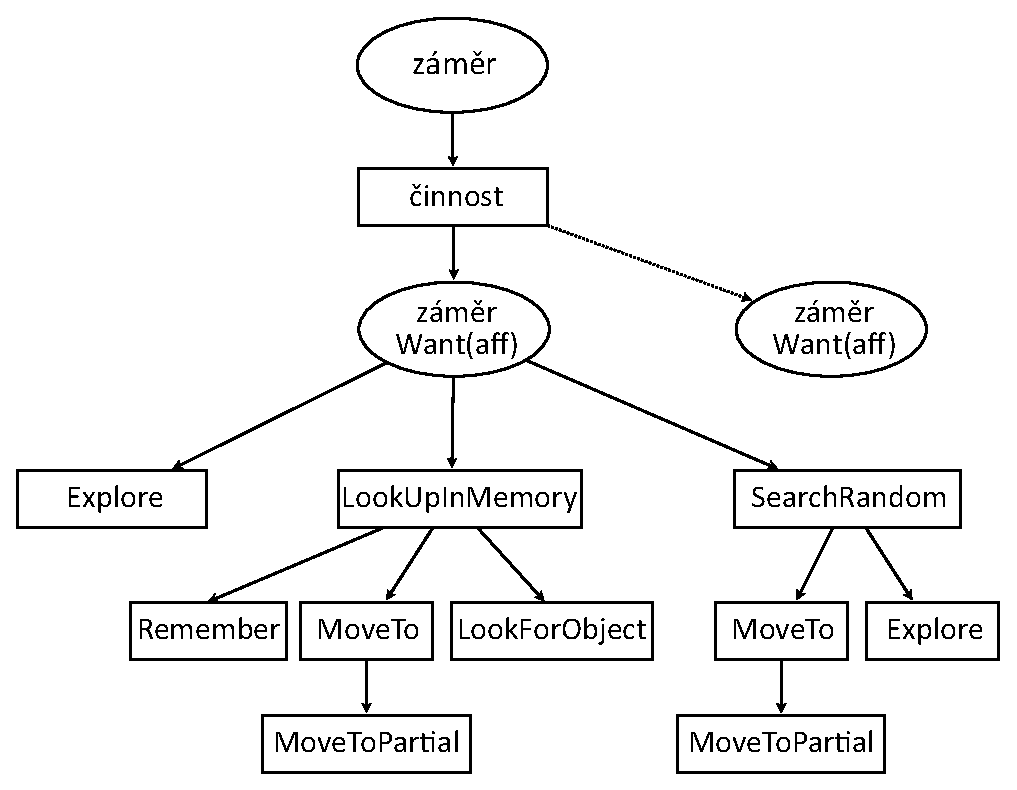
\includegraphics[width=0.8\textwidth]{img/and-or.ps}
  \caption{Strom chytr�ch akc� a jejich subakc�}
  \label{fig:smart-actions}
\end{figure}


Ka�d� tato �innost se skl�d� z n�kolika akc�, kter� mohou obsahovat dal�� subakce, a nen� mo�n� ji prov�st v jednom kroku simulace.
V��e zm�n�n� �innosti jsou tedy implementov�ny jako tzv. chytr� akce, kter� si pamatuj� aktu�ln� stav a dle n�j dok�� ur�it, jakou subakci m� agent vykonat.
Strom akc� a subakc� je na obr�zku \ref{fig:smart-actions}.
Nap�. pro n�hodn� hled�n� p�edm�tu je pou�ita chytr� akce \emph{SearchRandom}. Ta je schopn� ur�it, kam se agent m� p�esunout pomoc� dal�� chytr� akce \emph{MoveTo}.
Teprve akce \emph{MoveToPartial} je atomick� a lze ji prov�st v jednom kroku simulace.
\\

\begin{definition}[Maxim�ln� krok agenta]
Parametr modelu \param{maxim�ln� krok agenta} ur�uje maxim�ln� vzd�lenost, o kterou agent zm�n� svoji polohu v jednom kroku simulace.
\end{definition}


Chytr� akce jsou:

\begin{description}
  \item[MoveTo(x,y)] \hfill \\
  p�esun agenta na polohu $<x,y>$. Nejd��ve je nalezena cesta, pokud je sv�t konvexn� m�stnost, jedn� se o �se�ku; pokud sv�t nen� konvexn�, jsou pou�ity waypointy a cesta je lomen� ��ra. Ka�d� �se�ka je pak rovnom�rn� rozd�lena na krat�� ��sti tak, aby d�lka jej� nejdel�� ��sti byla men�� ne� \param{maxim�ln� krok agenta}. D�ky tomu se agent ka�d� kolo simulace posune jen o mal� kus.
  \item[SearchRandom(afordance)] \hfill \\
  n�hodn� hled�n� p�edm�tu s danou afordanc�. Agent m� u ka�d�ho way\-pointu ulo�en �as, kdy jej naposledy vid�l. Tato akce zajist�, �e agent postupn� nav�t�v� v�echny waypointy v po�ad� dle ulo�en�ho �asu. Za�ne t�m, kter� nevid�l nejd�le a skon�� u toho, kter� vid�l naposledy. Toto po�ad� je ur�eno na za��tku akce. K p�esunu mezi waypointy agent prov�d� chytrou akci MoveTo.
  \item[LookUpInMemory(afordance)] \hfill \\
  z�sk�n� p�edm�tu s danou afordanc� s vyu�it�m prostorov� mapy. Agent si nejd��ve vybav� p�edm�t s danou afordanc�, kter� si pamatuje nejl�pe (to ur�� prostorov� mapa). K tomutu p�edm�tu se p�esune pomoc� chytr� akce MoveTo. Pak spust� atomickou akci LookForObject, kter� je jen speci�ln�m p��padem akce Explore.
  \item[Execute(�innost)] \hfill \\
  proveden� �innosti. Tato akce je spu�t�na pouze tehdy, pokud �innost, kterou chce agent vykonat, m� ji� v�echny zdroje\footnote{V sou�asn� implementaci m� ka�d� �innost pouze jeden zdroj. Pokud by m�la v�ce, bylo by t�eba, aby agent um�l p�edm�ty p�en�et.}. Pak agent ov���, zda v�echny zdroje �innosti jsou dostupn�, tedy �e je v jejich bezprost�edn� bl�zkosti. Pokud ne, p�esune se k nim pomoc� chytr� akce MoveTo.
\end{description}


\begin{table}[h!]
\begin{center}
\begin{tabular}{lp{6cm}}\toprule[0.5pt]

Atomick� akce & Efekt \\

\midrule[0.2pt]

MoveToPartial(x,y) & p�esun na pozici x,y\\

ExecuteReal(�innost) & proveden� �innosti\\

Explore & rozhl�dnut� se po okol�\\

Remember(afordance) & vybaven� si p�edm�tu z prostorov� mapy, kter� m� danou afordanci\\

LookForObject(pam�ov� fantom) & vyhled�n� p�edm�tu odpov�daj�c�ho pam�ov�mu fantomu\\

\bottomrule[0.5pt]
\end{tabular}\\
\end{center}
\centering
\caption{Atomick� akce}
\label{tab:atomic-actions}
\end{table}



Sou��st� sv�ta je i mno�ina z�m�r� a �innost�, kter� agent m��e vykon�vat. Z�vis� toti� na p�edm�tech, resp. jejich afordanc�ch, kter� jsou ve sv�t� dostupn�.
Pokud by sv�t obsahoval p�li� mnoho z�m�r�, kter� nelze v dan�m sv�t� splnit,
bude se agent chovat hloup� a data, kter� bude dost�vat prostorov� mapa, budou sp�e n�hodn�, ne� aby p�ipom�nala lidsk� chov�n�.
Agent pak str�v� v�t�inu �asu pohybem mezi waypointy, jak je uk�z�no na obr�zku \ref{fig:waypoint-hell}, a hled�n�m p�edm�t� s afordancemi, kter� se ve sv�t� nenach�zej�.
Bude v�novat m�n� �asu a tedy i pozornosti ostatn�m p�edm�t�m.
\\

Na za��tku simulace je vygenerov�n agent�v sc�n��, tj. posloupnost z�m�r�, kterou agent st�le dokola prov�d�.
Sc�n�� z�le�� pouze na z�m�rech definovan�ch v r�mci sv�ta, aby bylo mo�n� prov�d�t testy modelu se stejn�m sc�n��em.
\\

\begin{figure}[h]
  \centering
  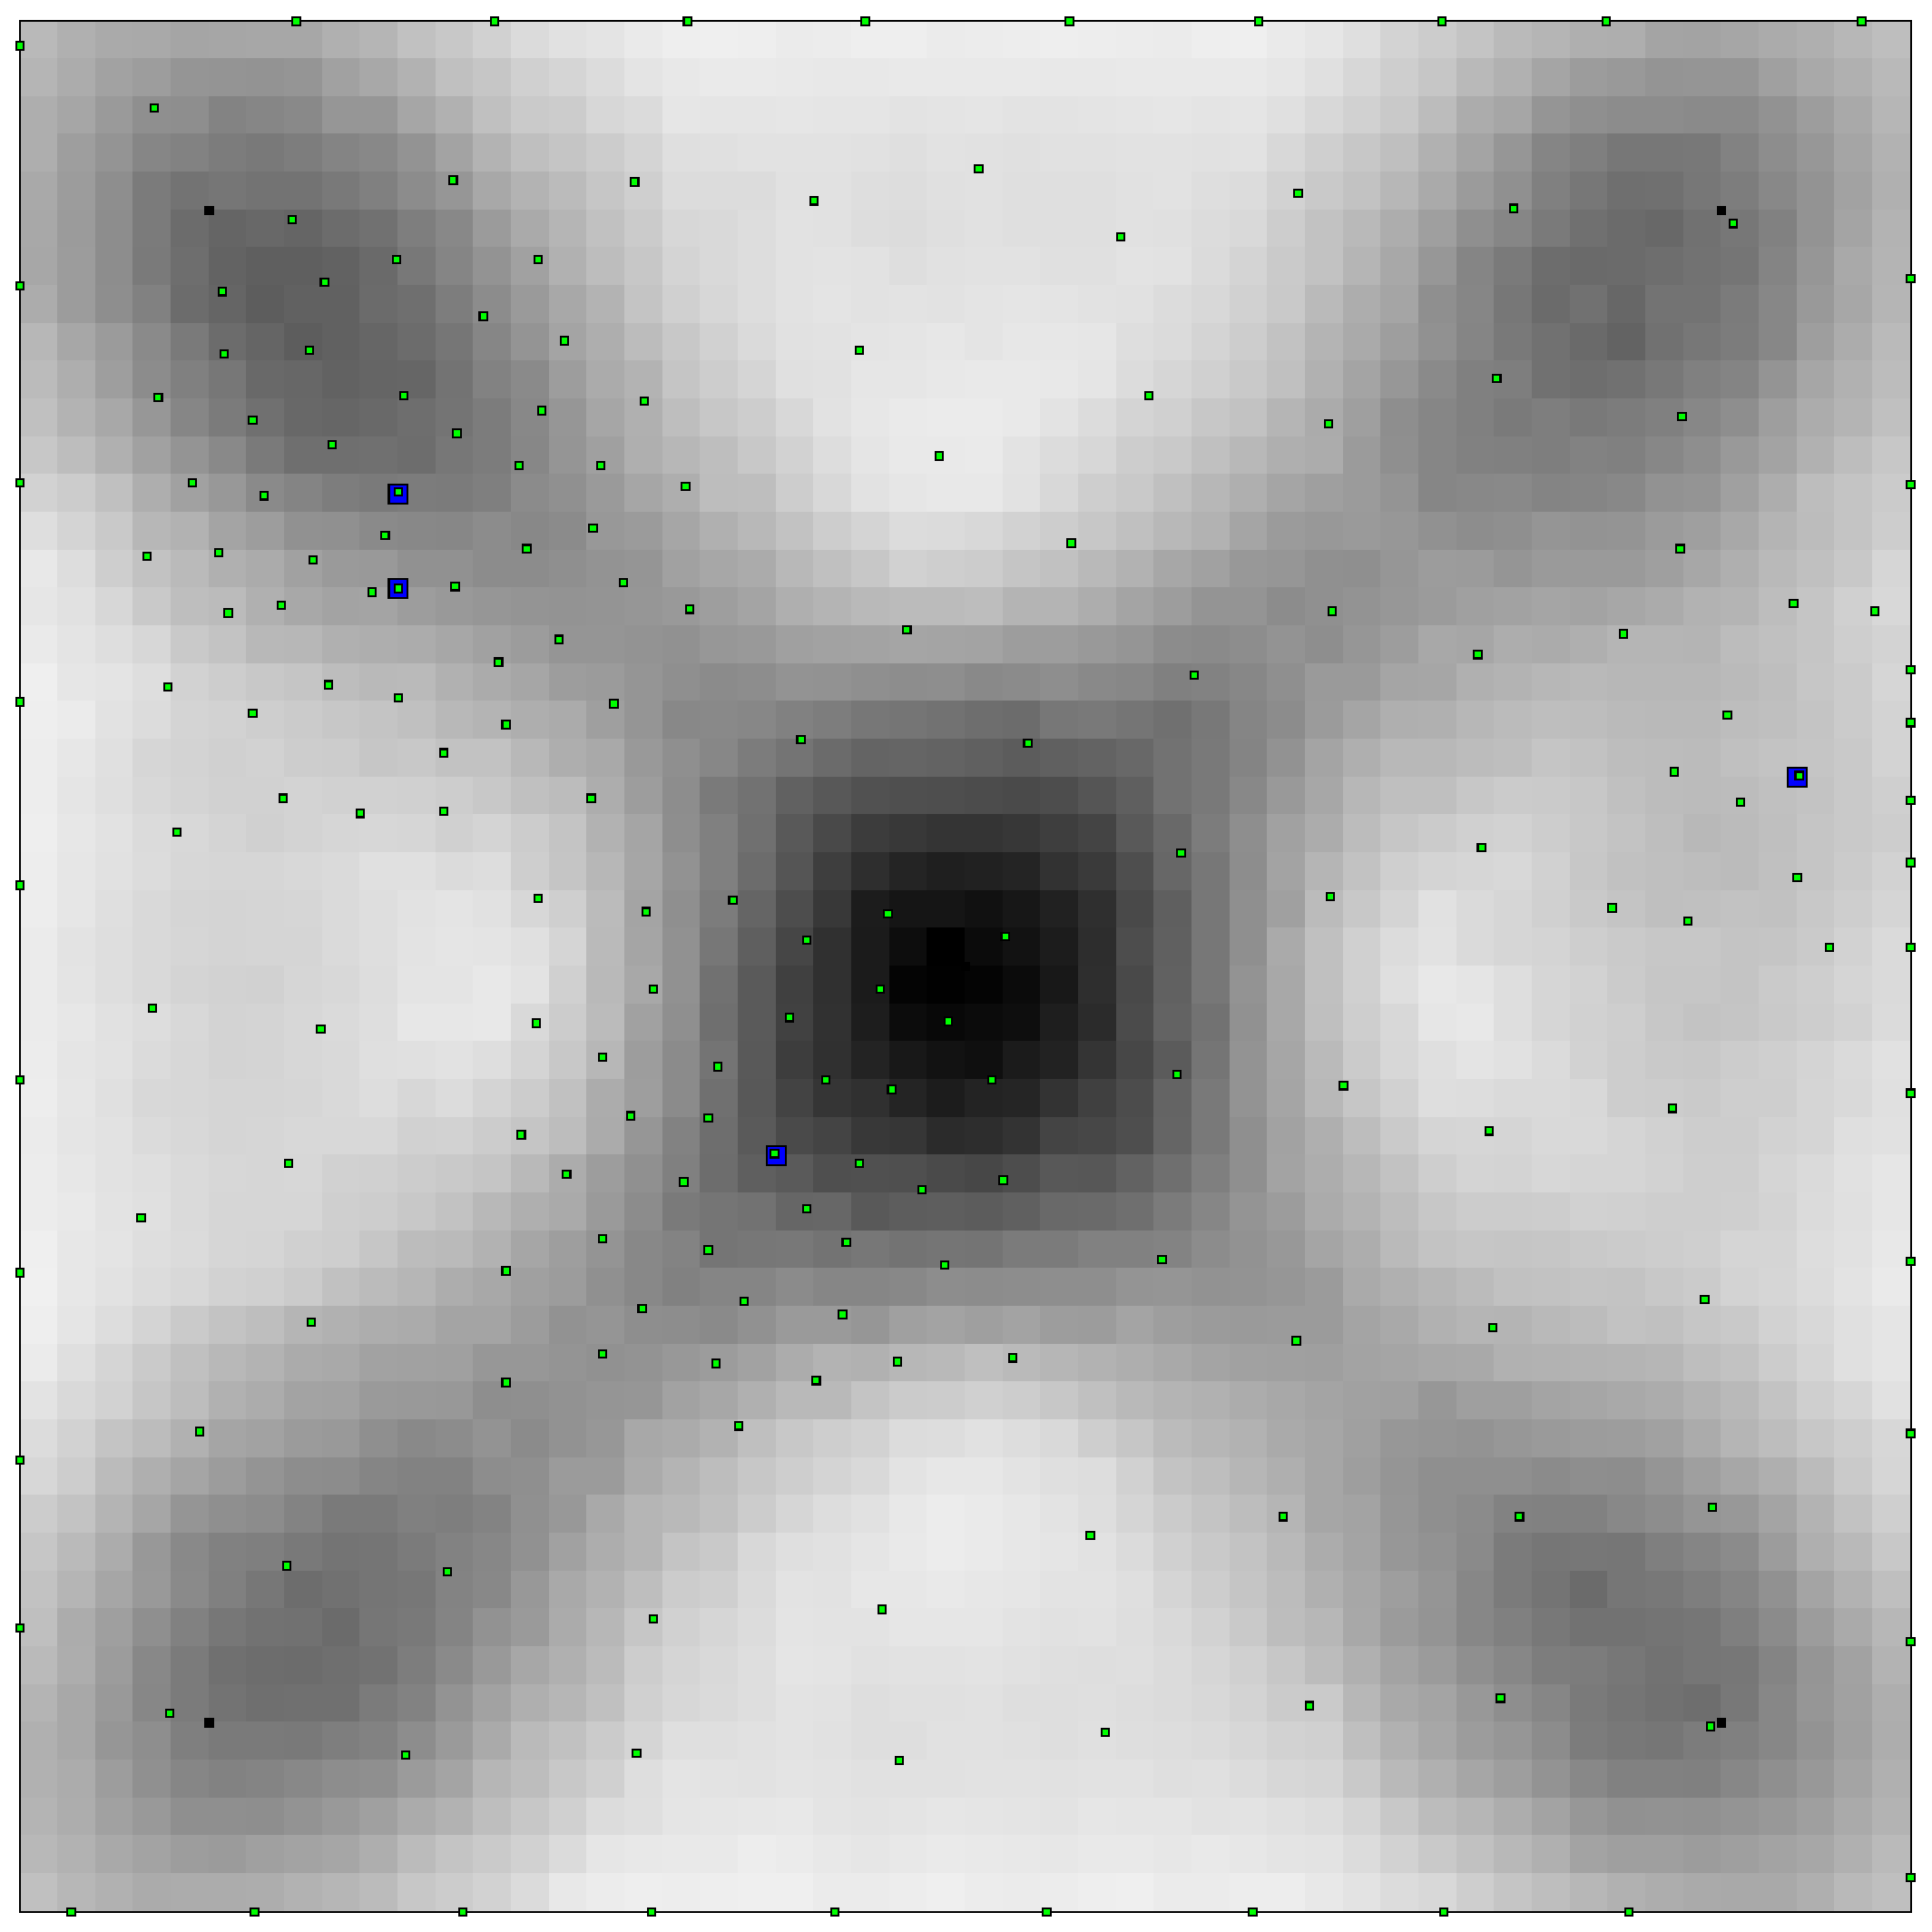
\includegraphics[width=0.4\textwidth]{img/waypoint-hell.eps}
  \caption{Mapa ukazuj�c�, jak sv�t agent vn�mal. B�l� m�sta nikdy nevid�l, ��m tmav��, t�m �ast�ji agent m�sto vid�l. Agent se pohyboval p�ev�n� po waypointech, kter� jsou v roz�ch a ve st�edu.}
  \label{fig:waypoint-hell}
\end{figure}

Pam� agenta je rozd�lena na kr�tkodobou a dlouhodobou. Dlouhodob� pam� v na�em p��pad� obsahuje pouze prostorovou mapu.
Kr�tkodob� pam�t se skl�d� ze t�� ��st�: procesn� ��sti, percep�n�ho pole a pam�ov� ��sti.
Procesn� ��st obsahuje pr�v� spl�ovan� z�m�r, prov�d�n� �innosti, chytr� akce a subakce, v�e uspo��dan� do stromu.
Percep�n� pole obsahuje odrazy zpozorovan�ch p�edm�t� z vn�j��ho sv�ta, tzv. fantomy.
Pam�ov� ��st obsahuje pam�ov� fantomy, odrazy p�edm�t� vybaven� z dlouhodob� pam�ti.
\\

\begin{definition}[Fantom]
Percep�n� pole obsahuje fantomy, tj. p�edm�ty, kter� agent pr�v� vn�m�.
Fantom je reprezentace agentovy my�lenky na p�edm�t.
M� svou intenzitu ur�uj�c� mno�stv� pozornosti, kterou agent fantomu v�nuje.
\end{definition}

\begin{definition}[Velikost percep�n�ho pole]

Agent m��e v jednom kroku simulace vid�t libovoln� mno�stv� p�edm�t�, ale je schopen jich vn�mat jen omezen� po�et.
Vych�z�me z kapacitn� teorie pozornosti, kter� ��k�, �e celkov� kapacita lidsk� pozornosti je omezen� \cite{litCapacityAtt}.
Po�et fantom�, kter� mohou b�t sou�asn� v percep�n�m poli, je d�n parametrem \param{velikost percep�n�ho pole}.
Tento parametr je pro v�echny testy roven magick�mu ��slu 7 dle experiment�ln�ch v�sledk� z \cite{lit7plusminus2}.
\end{definition}


V ka�d�m kroku simulace agent dostane mno�inu p�edm�t�, kter� vid�.
Ta je ur�ena z agentovy pozice a sm�ru, kter�m se d�v�, a z�vis� i na pr�v� prov�d�n� atomick� akci.
Proto�e zp�sob vn�m�n� okol� je pro model podstatn�, rozhodli jsme se implementovat s lehkou �pravou pokro�il� model z po��ta�ov� hry Thief \cite{litThief}.
V�sledn� model bere v potaz vzd�lenost p�edm�t� od agenta i to, jak moc by se agent musel oto�it, aby se d�val p��mo na n�.
\\

\begin{definition}[Zorn� pole]
Agent m� definov�na tzv. zorn� pole. Jsou p�edstavov�na kruhov�mi v�se�emi, jejich st�ed je v m�st� agenta, jsou orientov�ny sm�rem, kter�m se agent d�v�.
Zorn� pole je ur�eno polom�rem, �hlem a v�hou, kter� ur�uje m�ru vn�mavosti agenta na p�edm�ty v zorn�m poli.
\end{definition}

\begin{definition}[Viditelnost p�edm�tu]
V ka�d�m kroku m� ka�d� p�edm�t ur�enu svou viditelnost vzorcem \eqref{formula:viditelnost}, kde \emph{p} je p�edm�t, \emph{V} je mno�ina zorn�ch pol� agenta,
kter� agent pr�v� m�, a \(p \in v\) znamen�, �e p�edm�t le�� v zorn�m poli.
\end{definition}

\begin{equation} 
viditelnost(p) = 
\sum_{\substack{
   v \in V\\
   p \in v
  }}
  vaha(v)
\label{formula:viditelnost}
\end{equation}
\\

\begin{figure}
  \centering
  \subfloat[P�i atomick� akci Explore]{\label{fig:vcones-explore}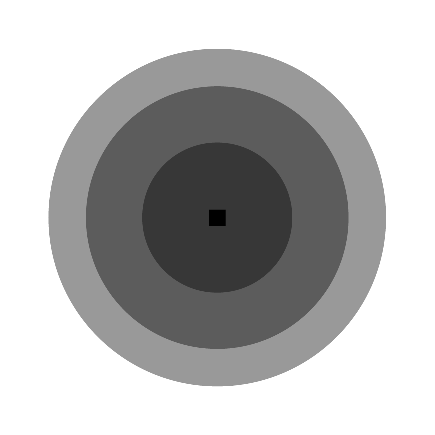
\includegraphics{img/vcones-explore.ps}}                
  \subfloat[P�i ostatn�ch akc�ch]{\label{fig:vcones-ostatni}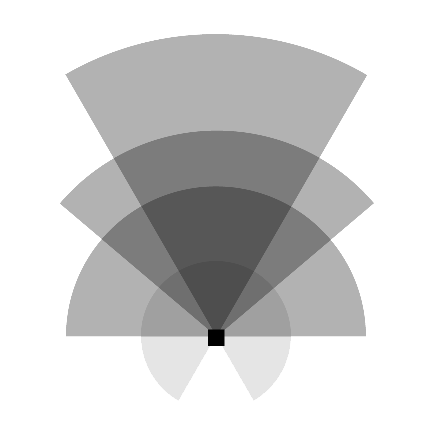
\includegraphics{img/vcones-normal.ps}}
  \caption{Zorn� pole ur�uj�c� agentovo vn�m�n�}
  \label{fig:vcones}
\end{figure}

Mno�ina zorn�ch pol� ur�uje agent�v zp�sob vn�m�n�. Toho jsme vyu�ili a definovali dv� r�zn� mno�iny zorn�ch pol�.
Jednu pro chv�le, kdy se agent rozhl�� (atomick� akce Explore) - obr�zek \ref{fig:vcones-explore}, a jednu pro zbyl� p��pady - obr�zek \ref{fig:vcones-ostatni}.
�hel 360� v prvn�m p��pad� simuluje to, �e p�i rozhl�en� se agent postupn� pod�v� do v�ech stran.
\\

P�edm�ty, kter� maj� kladnou viditelnost, agent vid� a jsou p�ed�ny k dal��mu zpracov�n� filtru pozornosti.
Pot� jsou vytvo�eny jejich fantomy a ty p�id�ny do percep�n�ho pole.
Pokud se v n�m udr�� alespo� jeden krok simulace, jsou p�ed�ny prostorov� map� a jejich fantomy procesn� ��sti.
\\

\begin{definition}[Aktu�ln� atraktivita p�edm�tu]
Filtr pozornosti upravuje aktu�ln� atraktivitu p�edm�t�. Atraktivita p�edm�tu m� dv� slo�ky, statickou a dynamickou.
Dynamick� atraktivita z�le�� na atomick� akci a �innosti, kterou agent pr�v� prov�d�.
Dynamick� atraktivita nab�v� hodnot z intervalu \(<0,1>\), viz tabulka \ref{tab:act-attr}.
Aktu�ln� atraktivita p�edm�tu je sou�in statick� a dynamick� atraktivity a jejich viditelnosti.
\end{definition}

\begin{table}[h!]
\begin{center}
\begin{tabular}{lcc}
\toprule[0.5pt]
\multirow{2}{*}{Atomick� akce} & \multicolumn{2}{c}{Dynamick� atraktivita p�edm�tu} \\
\cmidrule[0.2pt]{2-3}
 & bez po�adovan� afordance & s po�adovanou afordanc� \\

\midrule[0.2pt]

Remember & 0 & 0 \\

LookForObject & 0 & 0 \\

MoveToPartial & 1 & 1 \\

Explore & 0,5 & 1 \\

ExecuteReal & 0,5 & 0,75 \\

\bottomrule[0.5pt]
\end{tabular}\\
\end{center}
\centering
\caption{Dynamick� atraktivita p�edm�tu v z�vislosti na atomick� akci}
\label{tab:act-attr}
\end{table}


Pokud je fantom p�edm�tu ji� v percep�n�m poli, intenzita fantomu stoupne o aktu�ln� atraktivitu p�edm�tu.
Pokud nen�, je vytvo�en nov� fantom a p�id�n do percep�n�ho pole s intenzitou odpov�daj�c� aktu�ln� atraktivit� p�edm�tu.
P�id�n� fantomu v�ak nen� propagov�no hned d�le (do prostorov� mapy a procesn� ��sti).
Kdy� jsou zpracov�ny v�echny p�edm�ty, kter� agent v tomto kroku vid�l, jsou fantomy v percep�n�m poli se�azeny dle intenzity.
Pokud je fantom� v�ce ne� velikost percep�n�ho pole, jsou fantomy s nejni��� intenzitou z pole odstran�ny.
Teprve nyn� jsou nov� p�idan� fantomy p�ed�ny prostorov� map� a procesn�
��sti\footnote{Do prostorov� mapy a procesn� ��sti jsou tedy p�ed�ny pouze ty fantomy, kter� se ve�ly do percep�n�ho pole.}.
\\


\chapter{Model prostorov� mapy}

Agent popsan� v p�edchoz� kapitole m� dlouhodobou pam�, kter� obsahuje pouze prostorovou mapu.
Tu je mo�n� rozd�lit do dvou logick�ch ��st�: \emph{pam�ti na p�edm�ty} a \emph{vrstvy uzl�}.
\\

Vrstva uzl� �e�� rozlo�en� uzl� v prostoru, tedy pokryt� sv�ta uzly, kter� imituj� place cells.
M� za �kol m�nit hustotu uzl� dle zm�n sv�ta a vytv��et jejich hiearchii.
Pam� na p�edm�ty vyu��v� t�chto uzl� k ukl�d�n� informac� o poloze p�edm�t�\footnote{Vrstvu uzl� lze tak ch�pat jako pod��zenou pam�ti na p�edm�ty}.
\\

Zat�mco pam� na p�edm�ty je nez�visl� na velikosti sv�ta, vrstva uzl� je navr�ena pro jeden uzav�en� prostor, typicky m�stnost.
Z�rove� je pam� na p�edm�ty nez�visl� na  konkr�tn�ch mechanismech vrstvy uzl� a obr�cen�.
V�sledkem je, �e architekturu jedn� ��sti lze zm�nit bez z�sahu do druh�.
Druh�m v�sledkem je, �e model lze snadno roz���it pro sv�ty v�t�� ne� jeden uzav�en� prostor, pokud agent bude zn�t topologii sv�ta.
Toto roz���en� je podrobn�ji pops�no v sedm� kapitole.
\\

N�sleduj�c� podkapitola podrobn�ji popisuje pam� na p�edm�ty. Dal�� podkapitoly p�edstavuj� n�kolik model� vrstvy uzl�, kter� jsme postupn� navrhli.
\\
\section{Pam� na p�edm�ty} \label{chapter-pamet-predmety}

Pam� na p�edm�ty �e�� ukl�d�n� objekt� (a potencion�ln� dal��ch informac�) k uzl�m.
Tedy ukl�d� informace typu:
\emph{Objekt XY je v uzlu n42 s intenzitou 5,2}.
Pam� na p�edm�ty vych�z� z pr�ce Tom�e Korenka \cite{litKorenko}.
\\

\begin{definition}[Pam�ov� stopa p�edm�tu]
Pam� nepracuje p��mo s re�ln�mi p�edm�ty, ale vytv��� si jejich kopie, tj. \emph{pam�ov� stopy p�edm�t�}.
Pam�ov� stopa je reprezentace re�ln�ho p�edm�tu v agentov� dlouhodob� pam�ti, prostorov� map�.
Je to trojice \emph{$<$p�edm�t, intenzita, poloha$>$}, kde p�edm�t je odkaz na re�ln� p�edm�t;
intenzita ur�uje, jak dob�e si agent tento p�edm�t pamatuje, a poloha jsou sou�adnice, na kter�ch se agent domn�v�, �e se p�edm�t nach�z�.
Pro ka�d� re�ln� p�edm�t m� pam� nejv��e jednu pam�ovou stopu.
\end{definition}

\begin{definition}[Pam�ov� s�]
Mezi pam�ov�mi stopami p�edm�t� a uzly mapy je asociativn� s�, kter� se vytv��� v pr�b�hu simulace, dle toho, jak agent vn�m� p�edm�ty kolem sebe.
Pam�ov� s� je mno�ina trojic \emph{$<$uzel,stopa,intenzita$>$}, tedy vazeb mezi pam�ov�mi stopami a uzly prostorov� mapy, kter� maj� svou intenzitu.
Intenzita je nez�porn� re�ln� ��slo.
\end{definition}

\begin{table}[h!]
\begin{center}
\begin{tabular}{lp{9cm}}\toprule[0.5pt]
Typ vjemu & Zp�sob vzniku \\

\midrule[0.2pt]

ObjectNoticed & Agent vid� p�edm�t, kter� minul� krok simulace nevid�l \\

ObjectNoticedAgain & Agent vid� p�edm�t, kter� vid�l ji� v p�edchoz�m krok simulace \\

ObjectFound & Agent nalezl p�edm�t jako v�sledek chytr� akce LookUpInMemory \\

ObjectNotFound & Agent nenalezl p�edm�t tam, kde ho hledal p�i chytr� akci LookUpInMemory \\

\midrule[0.05pt]

ObjectUsed & Agent p�edm�t pou�il, tento vjem nen� vytv��en a zpracov�v�n v pr�b�hu vn�m�n�, ale p�i prov�d�n� atomick� akce ExecuteReal \\

\bottomrule[0.5pt]
\end{tabular}
\end{center}
\centering
\caption{Typy vjemu}
\label{tab:typy-vjemu}
\end{table}


\begin{definition}[Dosah u�en�]
Parametr modelu \param{dosah u�en�} ur�uje velikost okol� pam�ov� stopy p�i u�en� pam�ov� s�t�.
Do okol� padnou pouze uzly ve vzd�lenosti men�� ne� \param{dosah u�en�}.
\end{definition}


V ka�d�m kroku je pam�ti p�edlo�ena mno�ina vjem� (m��e b�t pr�zdn�). Vjem je trojice \emph{$<$p�edm�t,poloha,intenzita$>$}.
Vjem m� sv�j typ dan� ud�lost�, kterou byl vyvol�n, jejich p�ehled je v tabulce \ref{tab:typy-vjemu}.
Ka�d� typ m� ur�en� koeficient, kter�m je vyn�sobena intenzita vjemu p�ed jeho zpracov�n�m prostorovou mapou, tyto koeficienty jsou parametry modelu.
\\


Proces zpracov�n� vjemu prostorovou mapou je shrnut v algoritmu \ref{alg:zpracovani-vjemu}.
V prvn�m kroku je ur�ena pam�ov� stopa uchov�vaj�c� informaci o p�edm�tu. Pokud nen� nalezena, je vytvo�ena nov�.
\\

\begin{algorithm}[h!]
\caption{Zpracov�n� vjemu pam�t� na p�edm�ty}
\label{alg:zpracovani-vjemu}
\begin{algorithmic}[1]
\State ur�en� pam�ov� stopy p�edm�tu
\State zv��en� intenzity pam�ov� stopy o intenzitu vjemu
\State $nodes\gets$ v�echny uzly, do jejich� okol� vjem padl dle $dosah_{uceni}$
\ForAll{$n \in nodes$}
	\State $\Delta \eta \gets \eta(n, vjem)$ dle vzorce \eqref{formula:intenzita-vazby} \label{alg:spacemap-intensity}
	\State zv��en� intenzity vazby mezi pam�ovou stopou a uzlem $n$ o $\Delta \eta$
\EndFor
\State vjem je p�ed�n vrstv� uzl� k dal��mu zpracov�n�
\end{algorithmic}
\end{algorithm}

V kroku \ref{alg:spacemap-intensity} je ur�ena intenzita, o kterou bude zv��ena vazba mezi pam�ovou stopou a uzlem dle vzorce:

\begin{equation} 
\Delta \eta(node, vjem) = \eta(vjem) \times \frac{ norm( dist(node, vjem) ) }
{\sum_{\substack{
   n \in nodes
  }}
  norm( dist(n, vjem) )
} ,
\label{formula:intenzita-vazby}
\end{equation}
\\

kde \emph{nodes} je mno�ina v�ech uzl�, do jejich� okol� vjem padl, a $dist$ je vzd�lenost uzlu od polohy vjemu.
Funkce $norm$ je libovoln� klesaj�c� funkce maj�c� obor hodnot $<0,1>$, nap�. nep��m� �m�ra $norm(x) = 1/max(1,x)$ �i Gaussova funkce.
%��st algoritmu \ref{alg:zpracovani-vjemu} m��e b�t prov�d�na v r�mci vrstvy uzl�, nap�. v modelu Energy Layer.
\\

\begin{algorithm}[h!]
\caption{Vzpomenut� si na p�edm�t}
\label{alg:vzpomenuti}
\begin{algorithmic}[1]
\State Vybr�n� pam�ov� stopy s nejvy��� intenzitou, kter� m� po�adovanou affordanci
\State Aktualizace informace o poloze p�edm�tu v pam�ov� stop�
\State Pam�ov� stopa je p�ed�na pam�ov� ��sti kr�tkodob� pam�ti, kter� z n� vytvo�� pam�ov�ho fantoma
\end{algorithmic}
\end{algorithm}

Prostorov� mapa je schopna ur�it, kde se nach�zej� p�edm�ty, kter� agent p�edt�m vid�l. Tato informace je ulo�ena v d��ve zm�n�n� asociativn� s�ti.
��m bl�e je p�edm�t n�jak�mu uzlu mapy, t�m vy��� je intenzita vazby mezi nimi.
Kdy� agent hled� p�edm�t maj�c� n�jakou affordanci, provede se proces popsan� v algoritmu \ref{alg:vzpomenuti}. V kroku 2 je spo��t�na poloha p�edm�tu z informac� ulo�en�ch v asociativn� s�ti.
Poloha p�edm�tu je v�en� centroid v�ech uzl�, kter� maj� vazbu na pam�ovou stopu, v�hou je intenzita vazeb:
\\

\begin{equation} 
c_w(stopa) = \frac{\displaystyle \sum_{n \in stopa} n_{xy} \times \eta(vazba_n) }{\displaystyle \sum_{n \in stopa} \eta(vazba_n) }.
\label{formula:el-centroid-mista}
\end{equation}

\begin{definition}[Zapom�n�n� asociativn� s�t�]
V ka�d�m kroku simulace je sn�ena intenzita pam�ov�ch stop a
intenzita v�ech vazeb mezi pam�ov�mi stopami a uzly prostorov� mapy.
%(MemObjIntensityFadeOut, LinkMemObjToNodeFadeOut)
\end{definition}

\section{Vrstva uzl�}

Vrstva uzl� je ��st prostorov� mapy zodpov�dn� za rozlo�en� uzl� v prostoru a zm�nu jejich po�tu rozlo�en� v �ase.
D�le obsahuje mechanismy pro zm�nu po�tu uzl� a vytv��en� hiearchie.
\\

\begin{definition}[Okam�it� napln�nost uzlu]
Uzel prostorov� mapy m� vazby na pam�ov� stopy. Tyto vazby maj� svou intenzitu.
Okam�it� napln�nost uzlu je sou�et intenzit v�ech vazeb uzlu na pam�ov� stopy.
P�edstavuje m�ru nau�enosti uzlu, resp. m�ru jeho d�le�itosti pro pam� na p�edm�ty.
��m v�ce pam�ov�ch stop vyu��v� uzel a ��m intenzivn�j�� jsou, t�m m�n� by se m�la m�nit jeho poloha.
\end{definition}

Okam�it� napln�nost uzlu z�vis� p��mo na vazb�ch na pam�ov� stopy.
Kdy� kles� jejich intenzita, kles� stejn� i okam�it� napln�nost.
Nen� tedy mo�n� model dostate�n� parametrizovat tak, aby okam�it� napln�nost uzlu klesala rychleji �i pomaleji, ne� intenzita vazeb.
\\

\begin{definition}[Rychlost kles�n� napln�nosti]
Parametr modelu \param{rychlost kles�n� napln�nosti} uzlu ur�uje, jak rychle bude napln�nost uzlu klesat.
\end{definition}

\begin{definition}[Napln�nost uzlu]
Napln�nost je vlastnost uzlu, kter� z�le�� p��mo na \emph{okam�it� napln�nosti uzlu}, nem�n� se v�ak tak rychle, tj. m� ur�itou pam�.
Napln�nost uzlu $node$ budeme d�le ve vzorc�ch ozna�ovat znakem $\mu(node)$.
\end{definition}

P�i vytvo�en� nov�ho uzlu je jeho napln�nost rovna nule. V pr�b�hu simulace se m�n�, kdykoli je zv��ena intenzita vazby
mezi uzlem a pam�ovou stopou, je stejn� zv��ena i napln�nost uzlu.
V ka�d�m kroku simulace je napln�nost uzlu sn�ena o parametr \param{rychlost kles�n� napln�nosti}, nem��e ale klesnout pod nulu.
\\
\section{Model zalo�en� na Kohonenov� map�}

V�t�ina model� pam�ti, zm�n�n�ch v t�et� kapitole, vyu��v� samoorganiza�n� Kohonenovy mapy \cite{litKohonen}.
Kohonenova mapa je model neuronov� s�t� u��c� se bez u�itele, vyu��v� sout�n� strategii u�en�.
Neurony jsou v Kohonenov� map� uspo��d�ny do topologick� struktury, nej�ast�ji do dvourozm�rn� m��ky.
T�m je ur�eno, jak� neurony spolu soused�.
Okol�m neuronu $N_s(c)$ velikosti $s$ neuronu $c$ pak rozum�me jeho sousedy a dal�� neurony, jejich� vzd�lenost v topologii je men�� ne� $s$:

\begin{equation} 
N_s(c) = \{j:d(j,c)\leq s\},
\label{formula:km-okoli}
\end{equation}

kde $d(j,c)$ je vzd�lenost v topologick� struktu�e.
Neurony Kohonenovy mapy p�i u�en� sout�� o to, kter� z nich bude aktivn� p�i dan�m vstupu.
V�t�zn�m neuronem se stane ten, kter� se nejv�ce podob� vstupu. Jeho v�ha a v�hy neuron� v jeho okol� jsou upraveny.
Ostatn� neurony jsou neaktivn� a neu�� se. Kohonenova mapa a dal�� modely samoorganiza�n�ch map jsou pops�ny nap�. v \cite{litSimaNeruda}.
\\

\begin{figure}[h!]
  \centering
  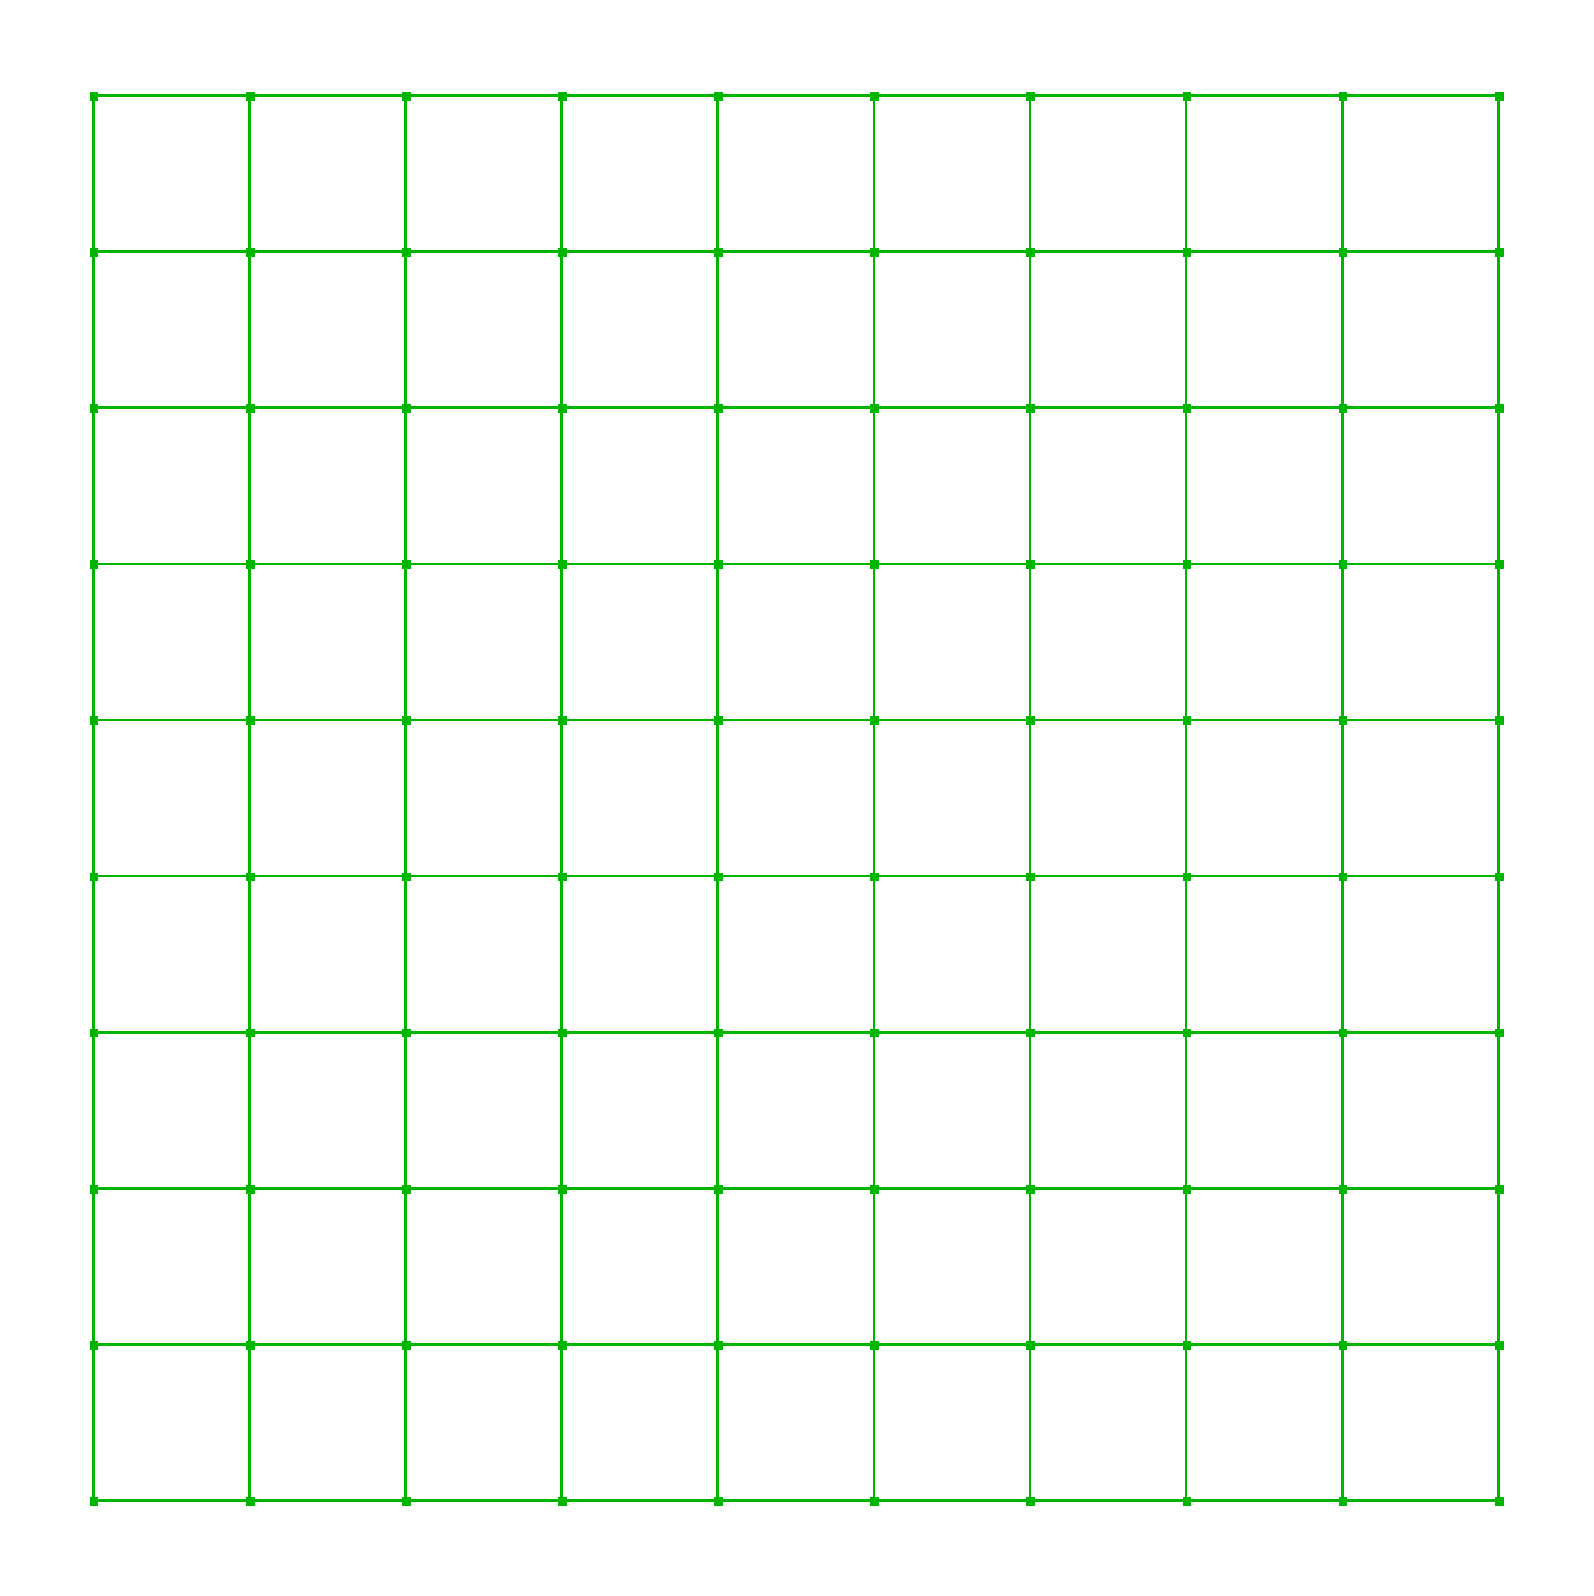
\includegraphics[width=0.5\textwidth]{img/kml/kml-start-grid.eps}
  \caption{Po��te�n� pokryt� sv�ta uzly uspo��dan�mi do �tvercov� m��ky.}
  \label{fig:kml-start}
\end{figure}

Kohonenova mapa by m�la spl�ovat na�e po�adavky. Um� rozm�stit uzly do hustoty odpov�daj�c� rozm�st�n� p�edm�t� v prostoru.
Um� se u�it online, ka�d� vjem agenta je mo�n� ch�pat jako prvek tr�novac� mno�iny dat.
Navrhli jsme tedy model vrstvy uzl� zalo�en� na Kohonenov� map�.
\\

\begin{definition}[Koeficient u�en�]
Rychlost u�en� Kohonenovy mapy je parametrizovateln�. Navr�en� model toho vyu��v�, koeficient u�en� ur�uje tuto rychlost.
\end{definition}


Na za��tku je prostor pokryt Kohonenovou mapou, uzly jsou uspo��d�ny do �tvercov� m��ky, viz obr�zek \ref{fig:kml-start}.
Poka�d�, kdy� je vjem p�ed�n ke zpracov�n�, provede se tr�nov�n� Kohonenovy mapy dle algoritmu \ref{alg:km-uceni}.
\\


\begin{algorithm}[h!]
\caption{Zpracov�n� vjemu}
\label{alg:km-uceni}
\begin{algorithmic}[1]
\State $node_{win} \gets$ vyhr�vaj�c� uzel (nejbli��� k poloze vjemu)
%\State $queue \gets \emptyset$
\State $queue \gets \{node_{win}\}$
\While{$queue\not= \emptyset$}
	\State $n \gets first(queue)$
	\State $queue \gets queue  \setminus \{n\}$
	\State zm�na polohy $n$ dle vzorce \ref{formula:km-uceni} \label{alg:km-uceni-vzorec}
	\State $queue \gets$ sousedi $n$ (pokud nebyli je�t� tr�nov�ni)
\EndWhile
\State vjem je p�ed�n vrstv� uzl� k dal��mu zpracov�n�
\end{algorithmic}
\end{algorithm}

Vyhr�vaj�c� uzel $node_{win}$ je ur�en dle vzd�lenosti mezi uzlem a vjemem:
\begin{equation}
node_{win} =\argmin_{node \in nodes} dist(node,vjem).
\end{equation}

V algoritmu je na ��dce \ref{alg:km-uceni-vzorec} zm�n�na poloha uzlu mapy. Uzel je posunut sm�rem k poloze vjemu o \(\Delta xy(n, vjem)\) dle vzorce:

\begin{equation} 
\Delta xy(n, vjem) = coef_{neighbour}(n, node) \times coef_{learn} \times dist(n, vjem),
\label{formula:km-uceni}
\end{equation}

kde \(coef_{neighbour}\) je vzd�lenost mezi vyhr�vaj�c�m uzlem a pr�v� tr�novan�m uzlem v Kohonenov� map�
 a \(coef_{learn}\) je koeficient u�en� Kohonenovy mapy.
Vzorec \eqref{formula:km-uceni} je analogi� u�en� Kohonenovy mapy.
\\

T�mto algoritmem by se m�la prostorov� mapa v pr�b�hu simulace nau�it rozm�st�n� p�edm�t� ve sv�t� a p�izp�sobit se mu.
Uzly mapy se postupn� p�esunou do m�st s velkou �etnost� vjem� a rozm�st�n� uzl� by se tak m�lo v �ase postupn� bl�it rozm�st�n� p�edm�t�.
\\

\begin{figure}[h!]
  \centering
  \subfloat[Po 1000 kroc�ch]{\label{fig:kml-preuceni-1}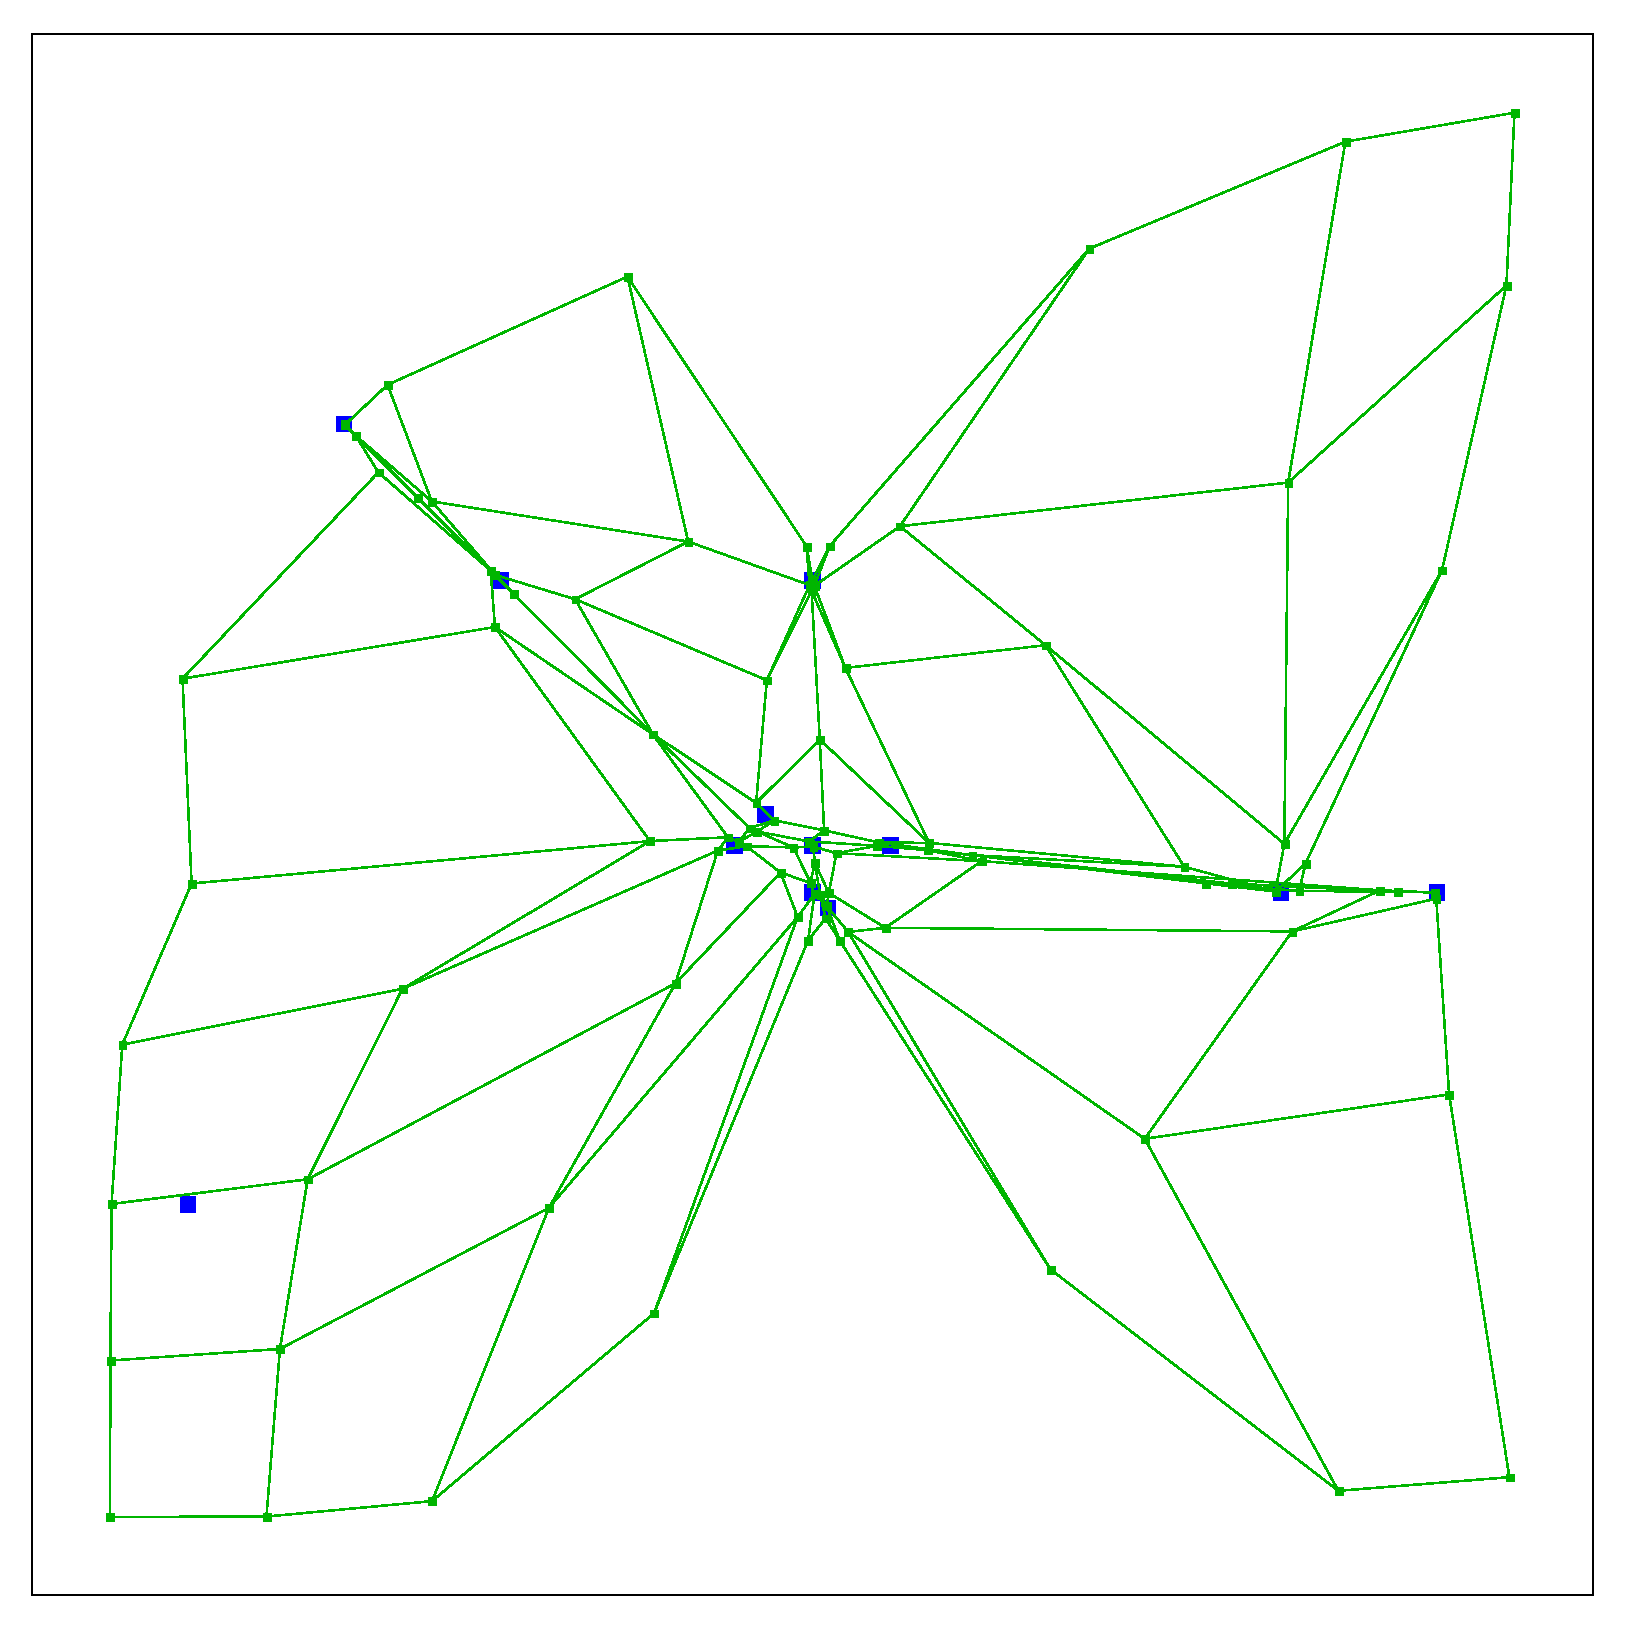
\includegraphics[width=0.5\textwidth]{img/kml/kml-preuceni-1.eps}}
  \subfloat[Po 4000 kroc�ch]{\label{fig:kml-preuceni-2}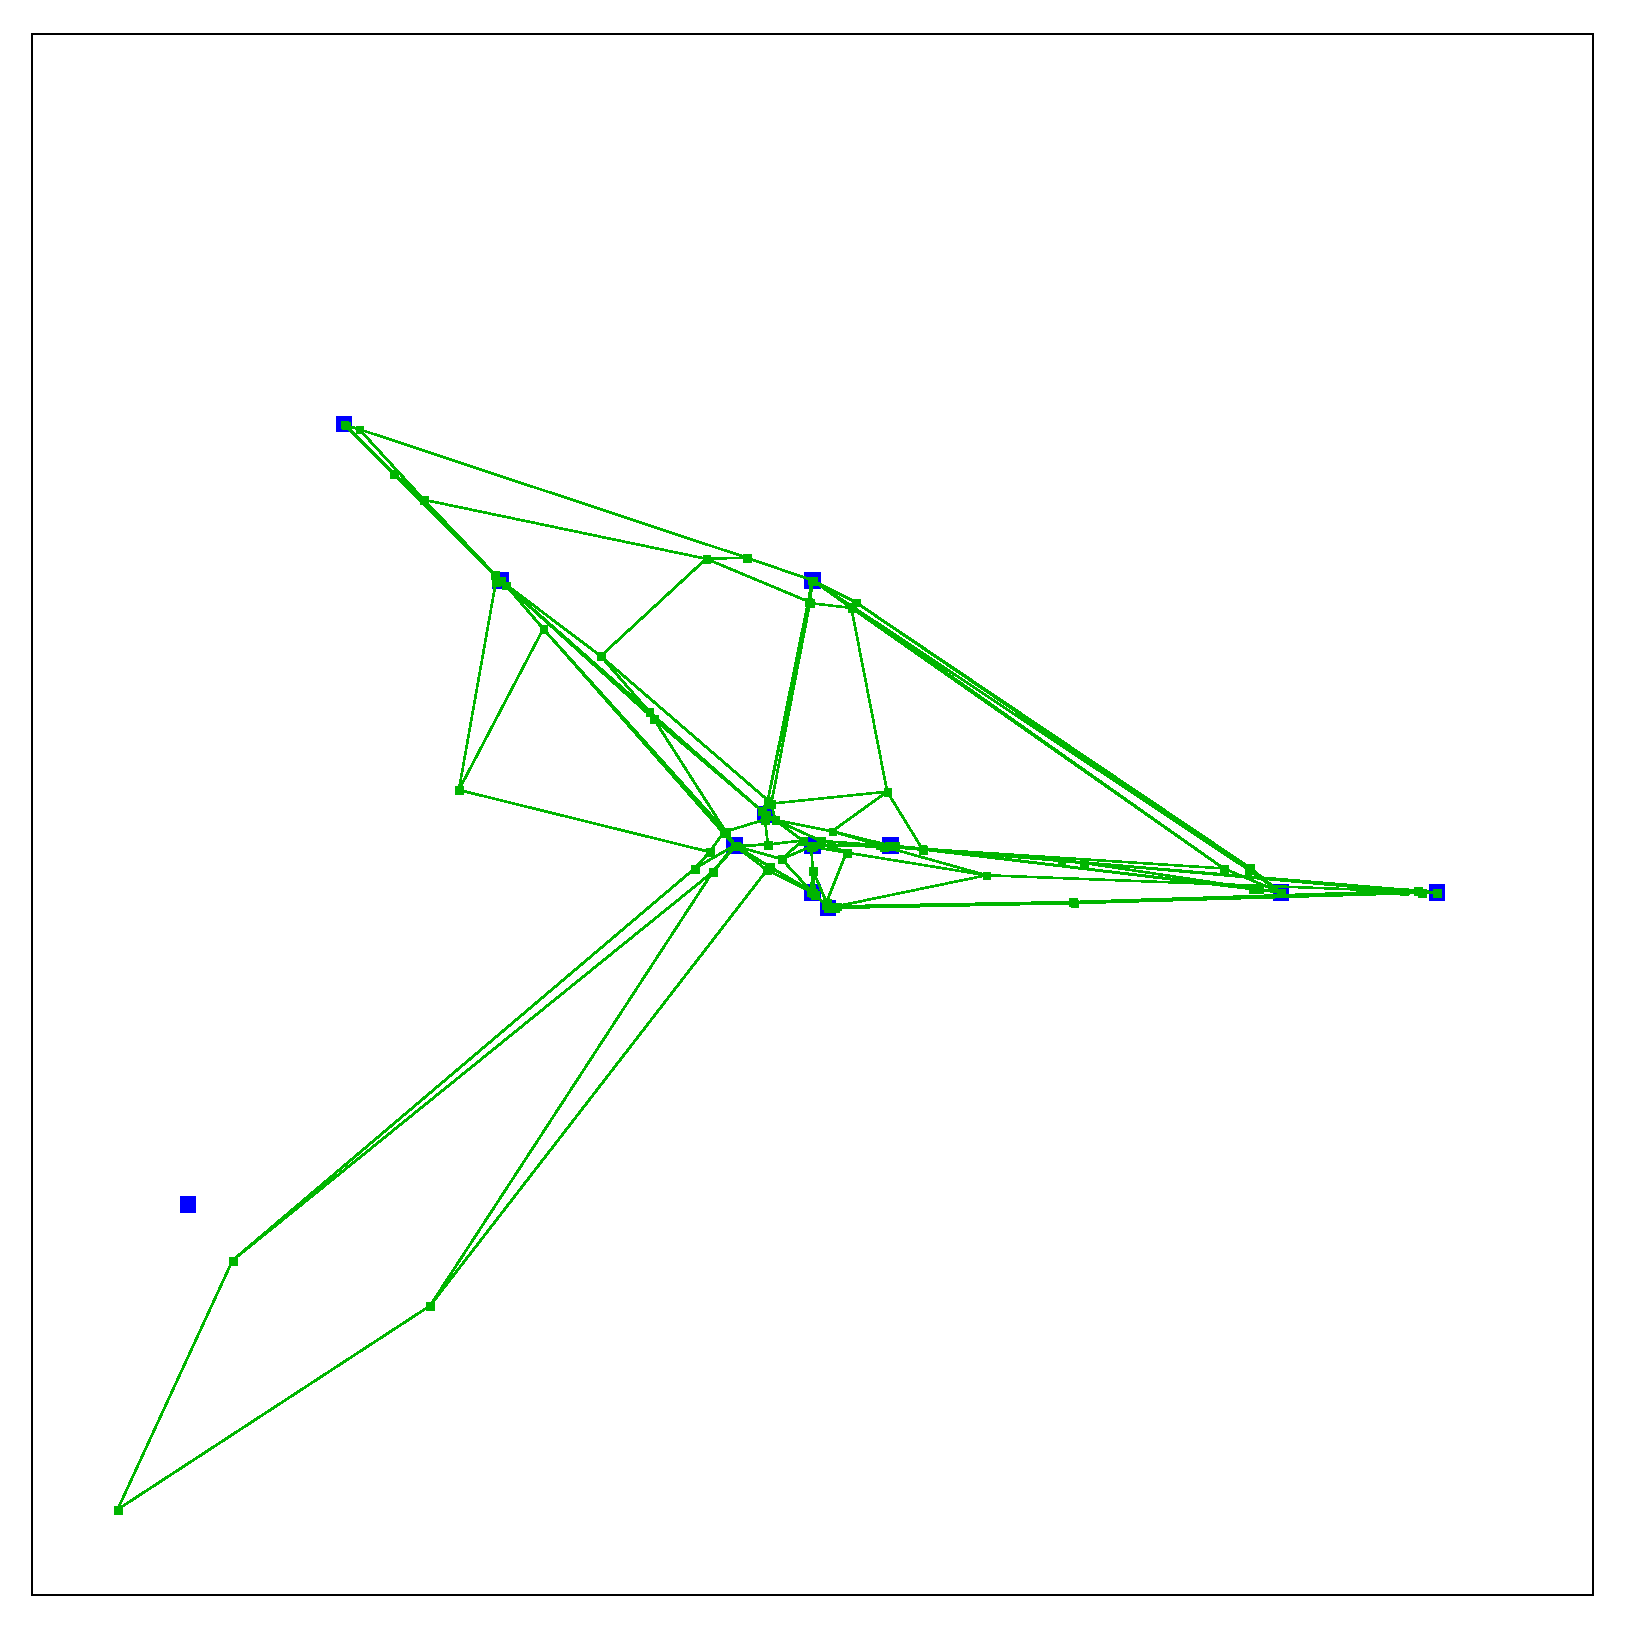
\includegraphics[width=0.5\textwidth]{img/kml/kml-preuceni-2.eps}}
  \caption{Test modelu a uk�zka jeho p�eu�en�}
  \label{fig:kml-preuceni}
\end{figure}

Test modelu (obr�zek \ref{fig:kml-preuceni}) uk�zal, �e k tomu skute�n� dojde, ale v�ce, ne� bychom cht�li.
Probl�m, kter� nastal je, �e se s� pro na�e pot�eby \uv{p�eu�ila}
 -- uzly se �asem v�echny p�esunuly k p�edm�t�m a prostor bez p�edm�t� z�stal pr�zdn�, bez uzl�.
Navrhli jsme dv� �e�en�:
\begin{CompactItemize}
\item Um�l� p�edm�ty - p�id�n� um�l�ch p�edm�t�, kter� se budou sna�it dr�et p�vodn� rozlo�en� uzl� Kohonenovy mapy
\item Odpudivost uzl� - uzly mapy se budou vz�jemn� odpuzovat, aby se nenahromadily v�echny v jednom m�st�
\end{CompactItemize}

V��e zm�n�n� �e�en� jsme vyzkou�eli v jednoduch� �tvercov� m�stnosti.
\\

\subsection{Um�l� p�edm�ty}
Toto �e�en� p�id�v� do sv�ta dal�� p�edm�ty, agent je nevyu��v� k pln�n� sv�ch z�m�r�, pouze je vn�m� a m�n� dle nich svou prostorovou mapu.
Um�l� p�edm�ty mus� m�t ni��� atraktivitu ne� re�ln� p�edm�ty, aby nem�ly na prostorovou mapu v�t�� vliv ne� opravdov� p�edm�ty.
\\

Um�l� p�edm�ty jsou do sv�ta p�id�ny na za��tku, p�i vytv��en� �tvercov� s�t�. V ka�d�m m�st�, kde je uzel s�t�, je vytvo�en jeden um�l� p�edm�t.
Agent je bude vn�mat stejn� jako ostatn� p�edm�ty, v pr�b�hu simulace budou k sob� p�itahovat uzly s�t� stejn� jako re�ln� p�edm�ty.
T�m by m�ly udr�et Kohonenovu mapu rozta�enou i v m�stech, kde re�ln� p�edm�ty nejsou.
\\

\begin{figure}[h!]
  \centering
  \subfloat[Po 500 kroc�ch]{\label{fig:kml-bo-1}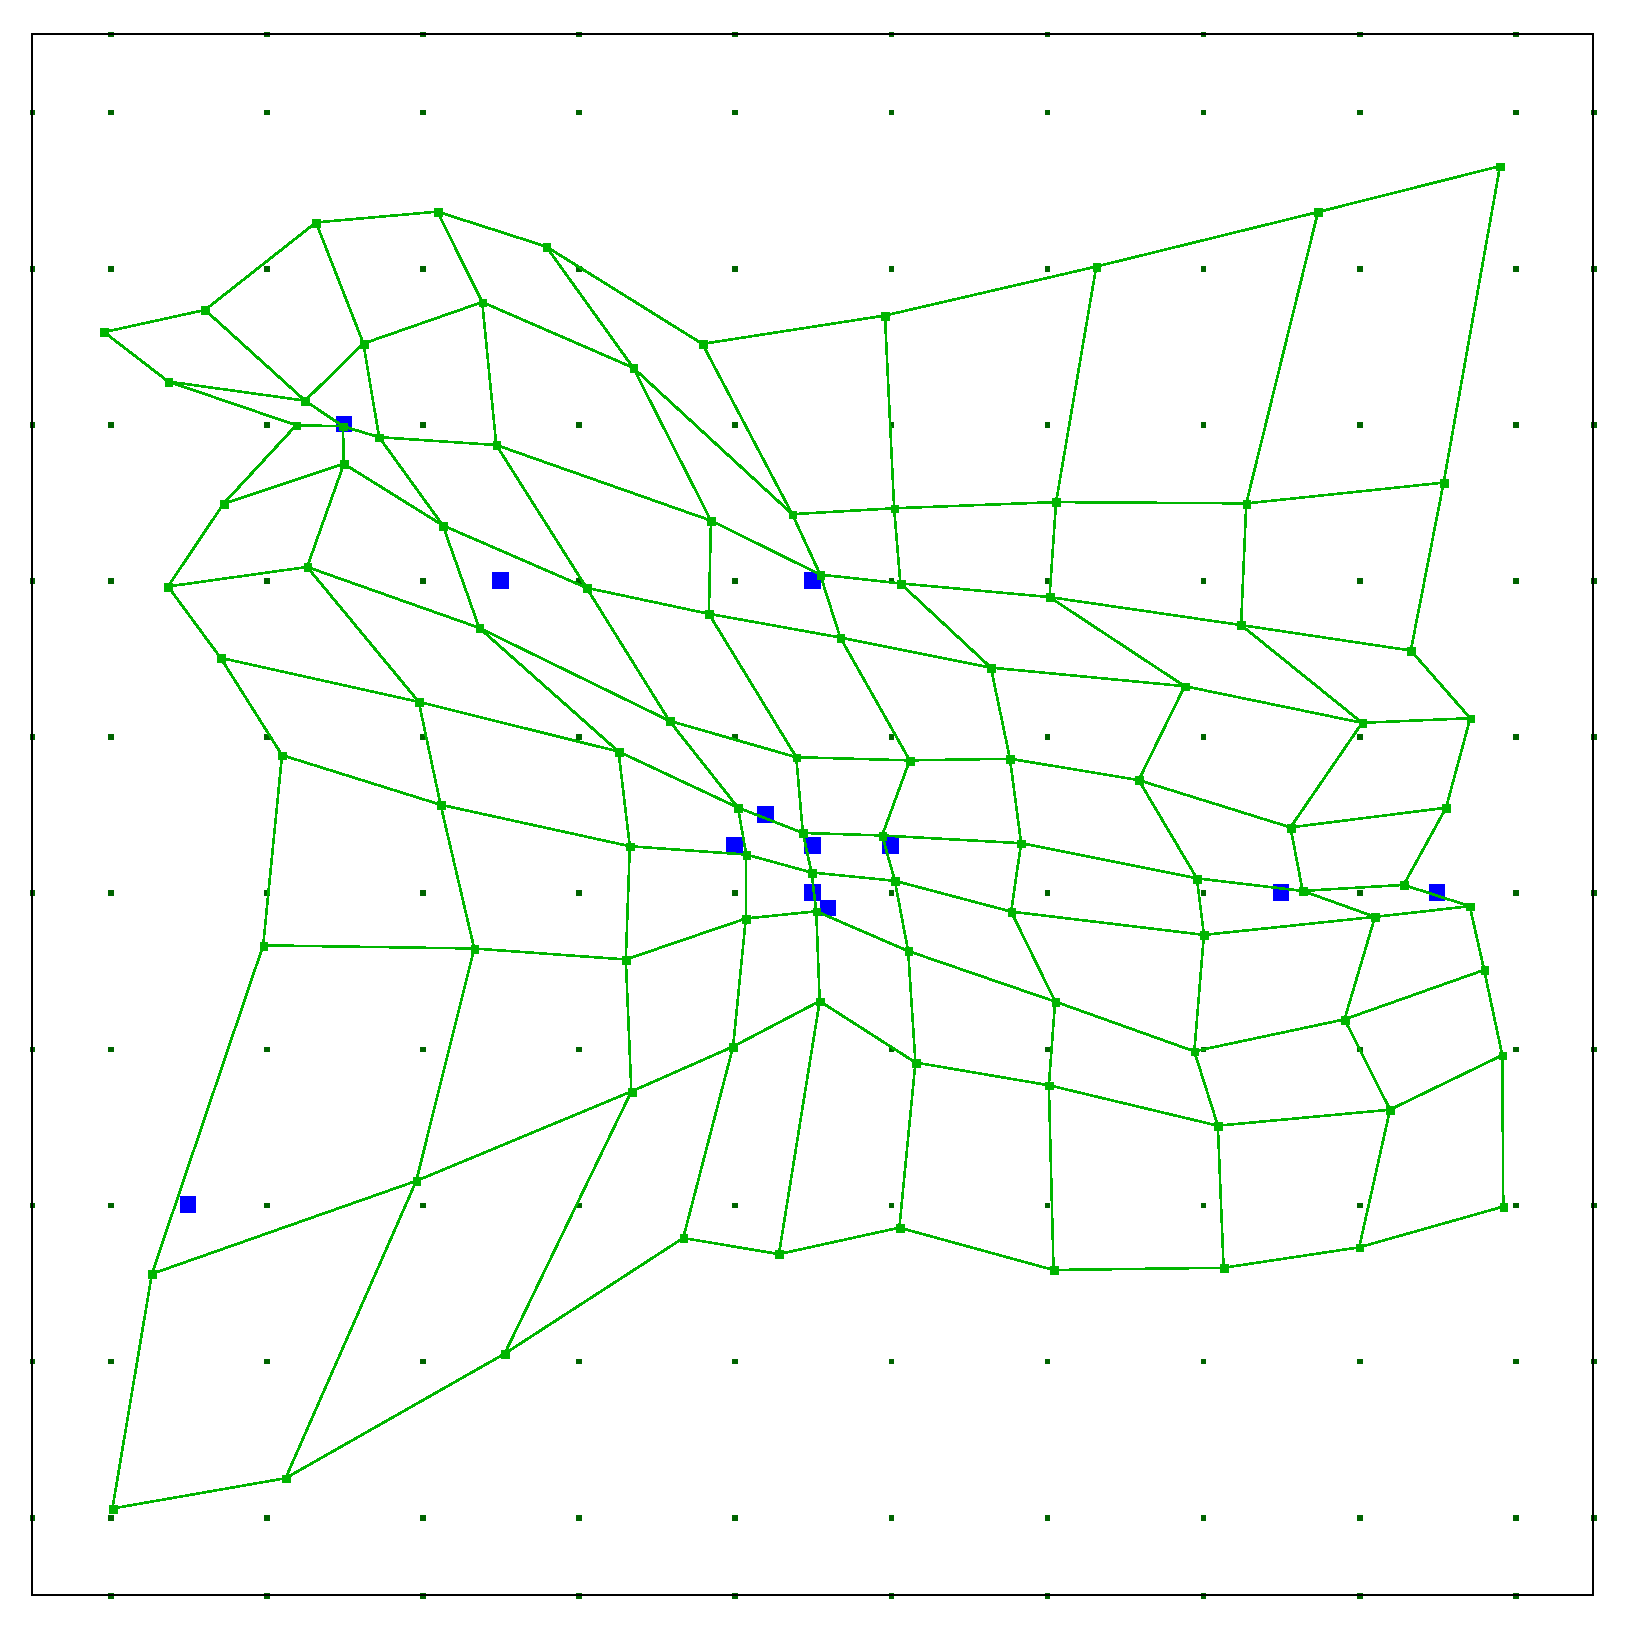
\includegraphics[width=0.5\textwidth]{img/kml/bo-0.5-0500.eps}}
  \subfloat[Po 1000 kroc�ch]{\label{fig:kml-bo-2}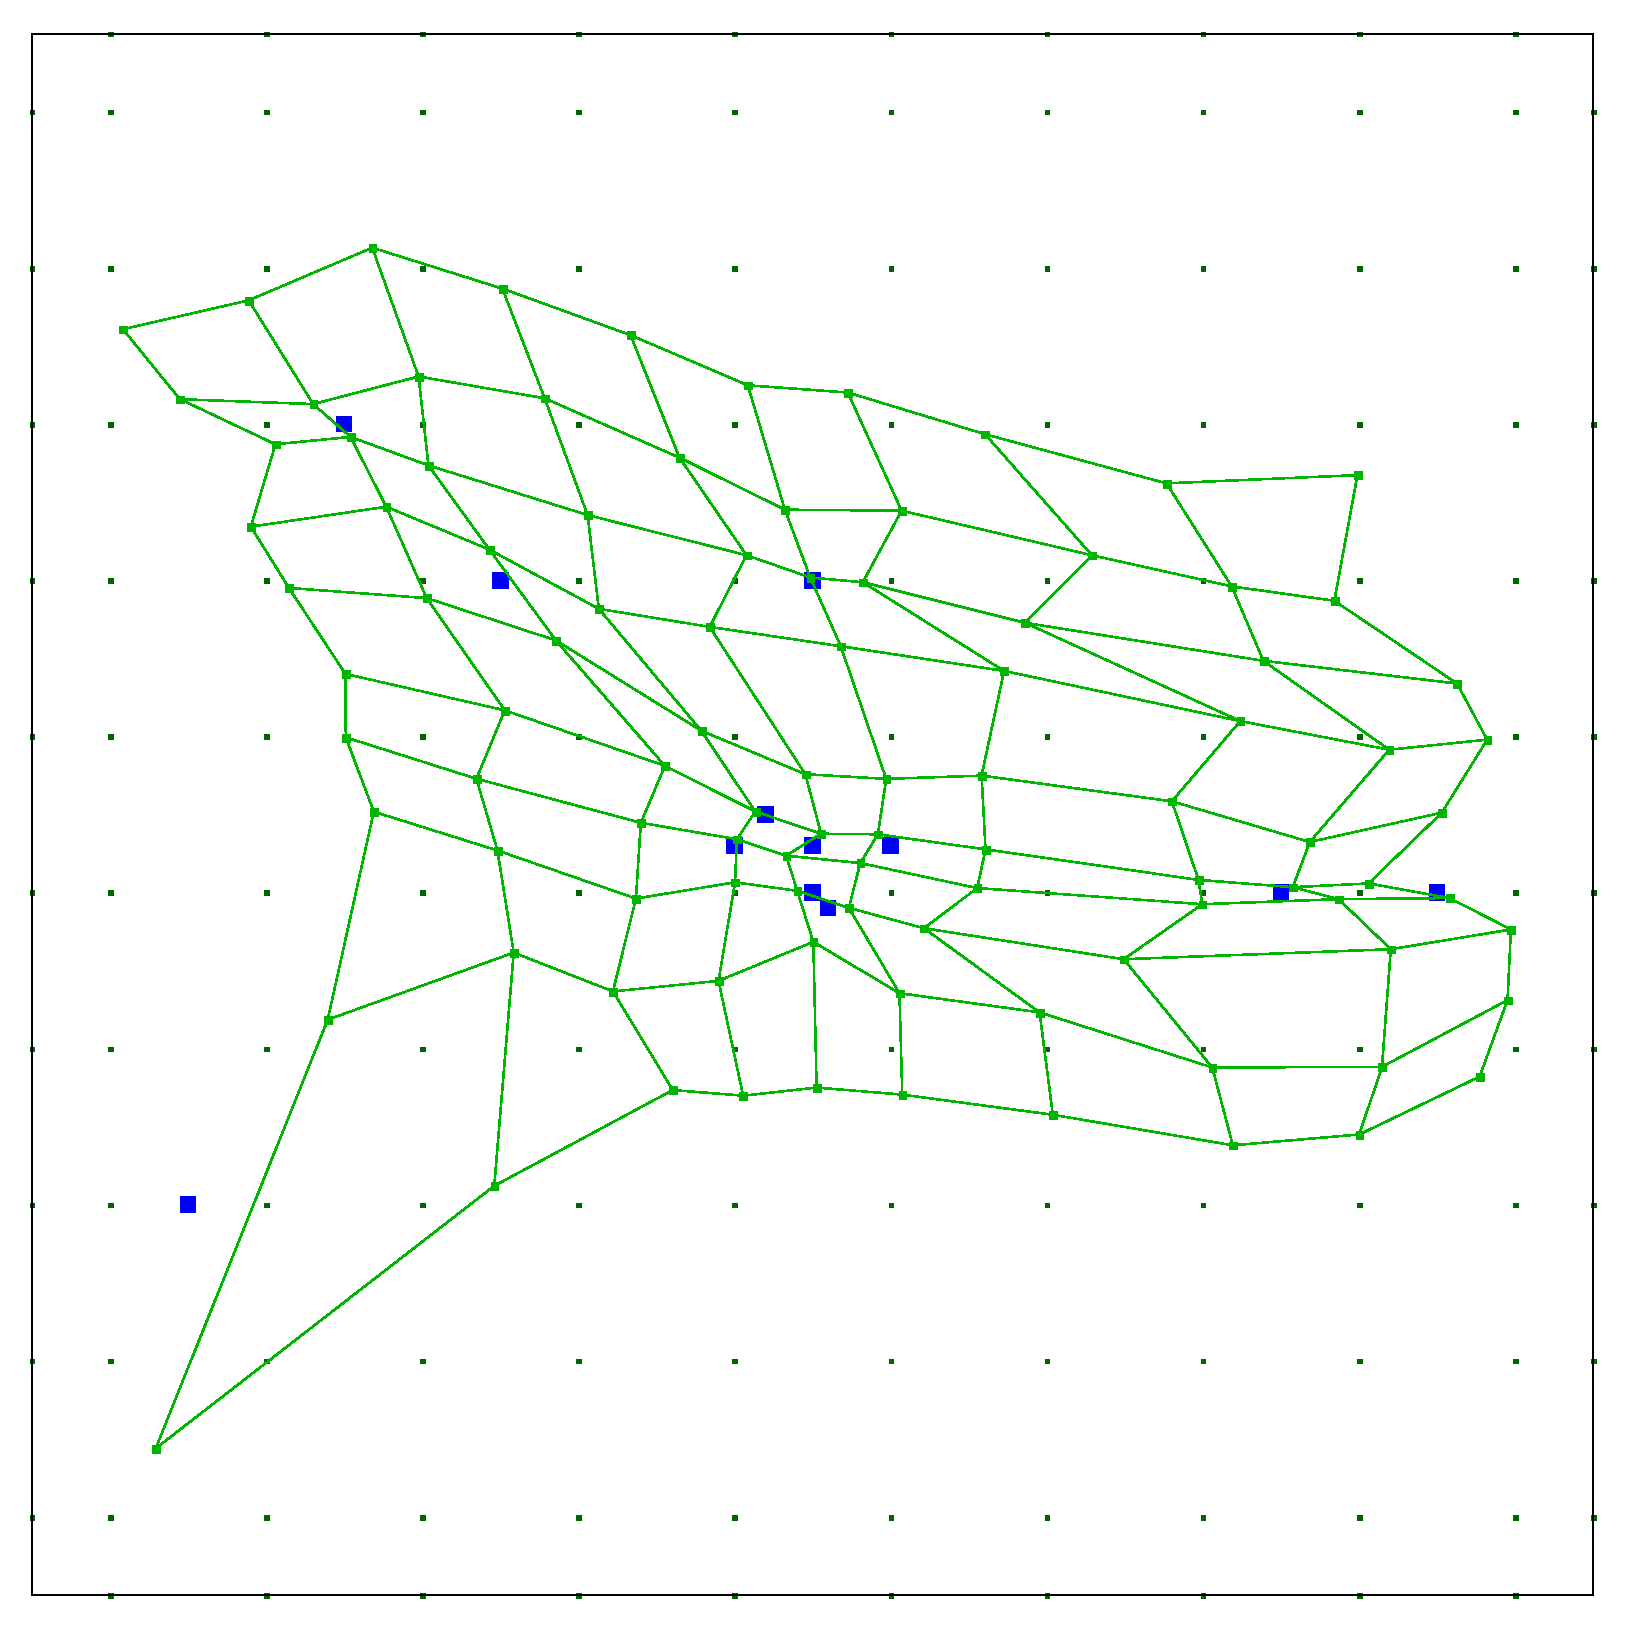
\includegraphics[width=0.5\textwidth]{img/kml/bo-0.5-1000.eps}}
  \caption{Test modelu s um�l�mi p�edm�ty}
  \label{fig:kml-baseobjs}
\end{figure}

V�sledek testu je na obr�zku \ref{fig:kml-baseobjs}\footnote{Dal�� v�sledky test� s r�znou hodnotou atraktivity um�l�ch p�edm�t� jsou na p�ilo�en�m DVD.}.
Uzly mapy se v pr�b�hu simulace stahuj� do st�edu m�stnosti.
Mapa se stahuje do st�edu m�stnosti bez ohledu na vliv um�l�ch p�edm�t�.
D�vodem je to, �e t�i�t� v�ech um�l�ch p�edm�t� je ve st�edu m�stnosti.
Tomu bychom mohli zabr�nit zv��en�m atraktivity um�l�ch p�edm�t�, kter� jsou na kraji m�stnosti.
Jednoduch�m protip��kladem takov�ho �e�en� je m�stnost, kter� bude m�t objekty pouze na kraji (na zdech, v roz�ch).
Pak bychom pot�ebovali zv��it atraktivitu um�l�ch p�edm�t� uprost�ed m�stnosti resp. obecn� bychom museli zv��it atraktivitu um�l�ch p�edm�t� v m�stech,
kde nejsou re�ln� p�edm�ty.
T�m jsme p�evedli p�vodn� probl�m hled�n� oblast� s vy���m po�tem p�edm�t� na probl�m opa�n�, tj. na hled�n� oblast� bez p�edm�t�.
�e�en� s pou�it�m um�l�ch p�edm�t� tedy nevyhovuje.
\\

\subsection{Odpudivost uzl�} \label{s:km-odpudivost}
Do modelu jsme p�idali vz�jemnou odpudivost uzl� s�t�. V ka�d�m kroku simulace se uzly, kter� jsou p��li� bl�zko u sebe, odpuzuj�.

\begin{definition}[S�la odpudivosti]
Parametr modelu \param{s�la odpudivosti} ur�uje m�ru s jakou se budou uzly odpuzovat.
\end{definition}


Vz�jemn� odpudivost dvou uzl� z�vis� na \param{s�le odpudivosti}, na vzd�lenosti uzl� a jejich napln�nosti.
Uzel s vysokou napln�nost� se bude nach�zet v m�st�, kde je hodn� p�edm�t�.
V takov�ch m�stech by hustota uzl� m�la b�t v�t��, a proto je nutn�, aby v takov�ch m�stech byla vz�jemn� odpudivost uzl� men��.
\\

\begin{equation} 
odpudivost(n_i, n_j) = \frac{ sila_{odpudivost} }{ dist(n_i, n_j)^2 \times \mu(n_i) \times \mu(n_j) } 
\label{formula:km-odpudivost}
\end{equation}
\\

Napln�nost uzlu lze p�i ur�ov�n� vz�jemn� odpudivosti ch�pat jako analogii k hmotnosti t�les, s t�m rozd�lem,
�e odpudivost dvou uzl� je nep��mo �m�rn� sou�inu jejich napln�nost�. Odpudivost je d�na vzorcem \eqref{formula:km-odpudivost},
kde $sila_{odpudivost}$ je parametr \param{s�la odpudivosti}.
V ka�d�m kroku simulace je spo�tena vz�jemn� odpudivost uzl�. T�m jsou ur�eny v�echny odpudiv� s�ly, kter� na uzly p�sob�.
Poloha uzl� je pak upravena dle t�chto sil:
\\

\begin{equation} 
\Delta_{xy}(node) = \frac{
\sum_{\substack{
   n \in nodes
  }}
  odpudivost(n, node)
}{ max(1, \mu(node)) }
\label{formula:el-odpudivost}.
\end{equation}
\\


\begin{figure}[h!]
  \centering
  \subfloat[Cel� m�stnost s nazna�en�m v��ezem]{\label{fig:kml-ag-cele}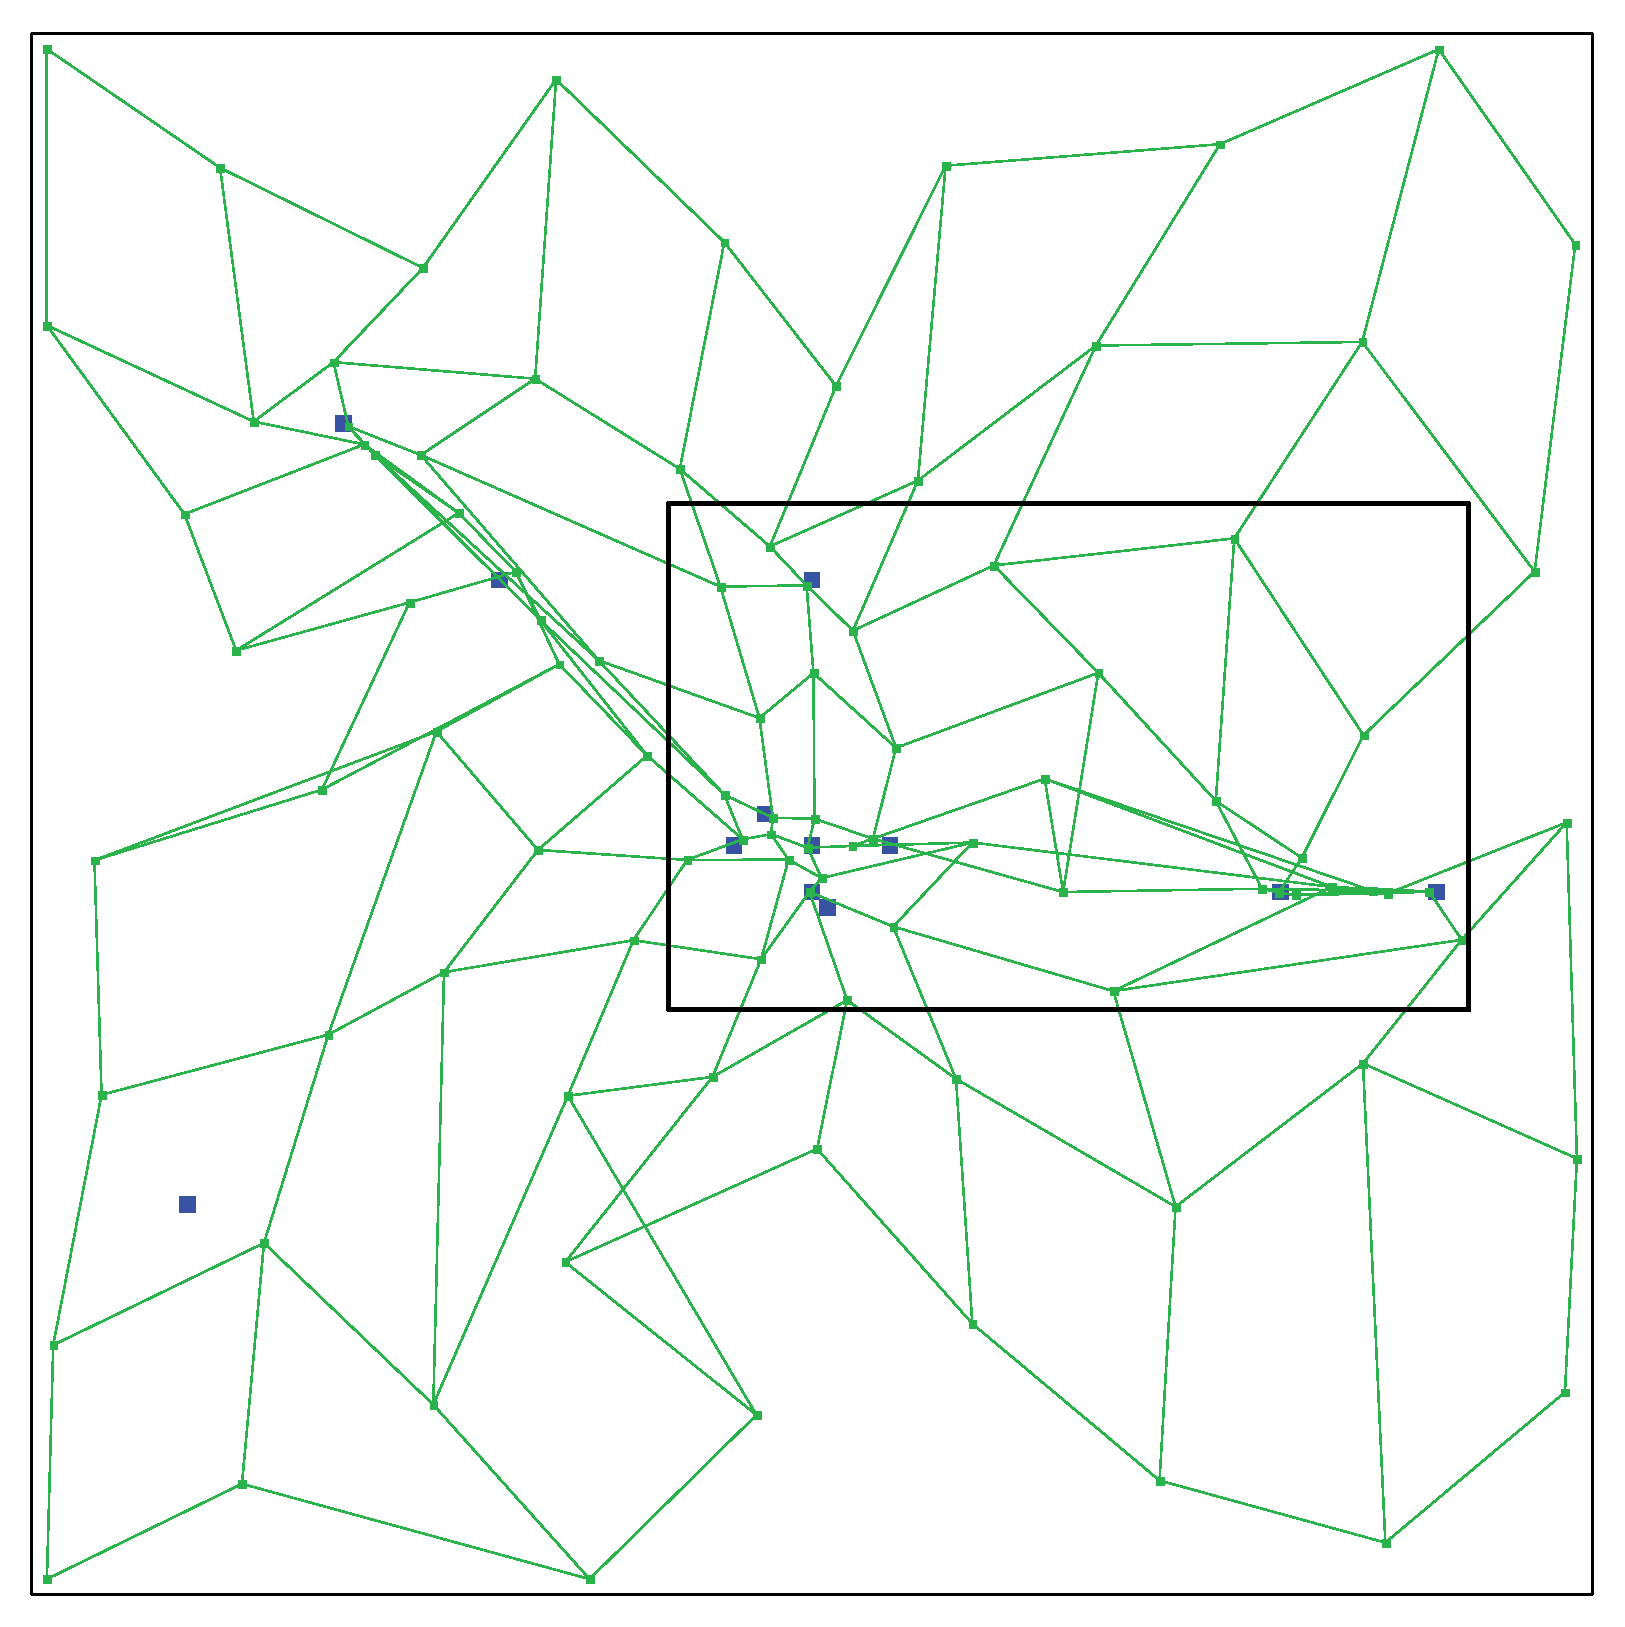
\includegraphics[height=0.36\textwidth]{img/kml/ag-cele.eps}}
  \quad
  \subfloat[V��ez]{\label{fig:kml-ag-vyrez}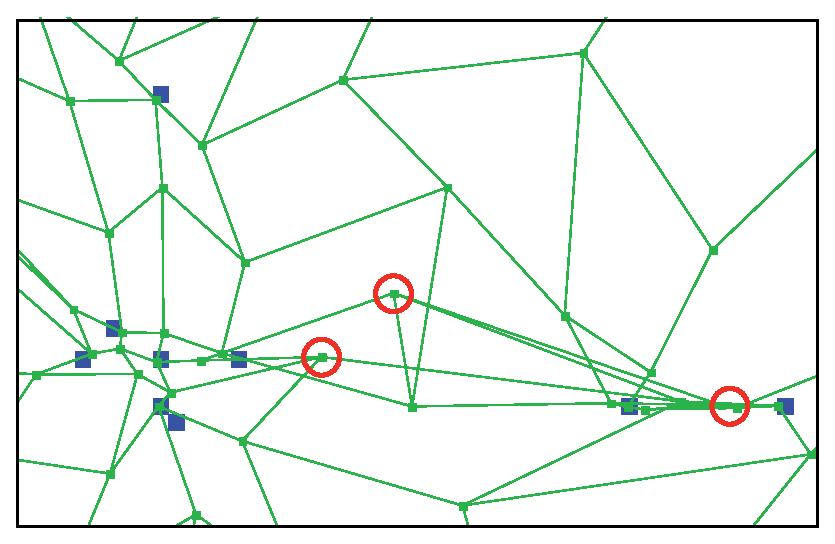
\includegraphics[height=0.36\textwidth]{img/kml/ag-vyrez.eps}}
  \caption{Test modelu s odpudivost� uzl�}
  \label{fig:kml-ag}
\end{figure}

V�sledek testu je na obr�zku \ref{fig:kml-ag}\footnote{Dal�� v�sledky test� s r�znou hodnotou s�ly odpudivosti jsou na p�ilo�en�m DVD.}.
Ukazuje, �e odpudivost skute�n� rozprost�e uzly po cel� m�stnosti.
Objevil se v�ak jin� probl�m -- odpudiv� s�ly deformuj� Kohonenovu mapu do stavu, kdy jej� n�sleduj�c� u�en� ned�v� smysl.
S� se p�ekrout� tak, �e uzly (na obr�zku \ref{fig:kml-ag} �erven� vyzna�en�), kter� jsou ve virtu�ln�m sv�t� vedle sebe, jsou v s�ti daleko od sebe a obr�cen�.
\\

D��ve zm�n�n� probl�m p�eu�en� skute�n� nastal a dv� rozd�ln� �e�en� jej nedok�zala uspokojiv� vy�e�it. Model zalo�en� na Kohonenov� map� jsme tedy zam�tli.
\\
\section{Gravita�n� model}

Inspirov�ni pou�it�m odpudivosti v p�edchoz�m modelu, rozhodli jsme se vytvo�it model zalo�en� pouze na p�ita�livosti a odpudivosti.
Tedy uzly mapy jsou p�itahov�ny k p�em�t�m a z�rove� se vz�jemn� odpuzuj�. Ob� s�ly berou v potaz napln�nost uzlu.
\\

Model d�le obsahuje my�lenku, �e i kdy� �lov�k vn�m� p�edm�ty v jeden okam�ik, ukl�d�n� do pam�ti prob�h� postupn�. 
Tato my�lenka je do modelu zapracov�na tak, �e vjem je sice dod�n prostorov� map� v jeden konkr�tn� krok simulace,
ale mapa si jej ulo�� a u�� se dle n�j n�kolik n�sleduj�c�ch krok�.
\\



\subsection{Vytvo�en� vrstvy uzl�}

Na za��tku simulace si agent vytvo�� ??prvotn�?? prostorovou mapu, kter� neobsahuje ��dn� informace o p�edm�tech ani jejich rozlo�en� ve sv�t�.
Obsahuje uzly, rozm�st�n� pouze dle geometrie m�stnosti. Jejich po�et a zp�sob rozlo�en� je parametrizov�n.
\\

\begin{definition}[Po��te�n� odchylka mapy]
Uzly mohou b�t um�st�ny zcela n�hodn� �i pravideln� ve �tvercov� m��ce s n�hodnou odchylkou.
N�hodn� odchylka m��e b�t i nulov�, ��m� je dosa�eno pravideln�ho rozlo�en� uzl�.
Uk�zky po��te�n�ho rozlo�en� uzl� jsou na obr�zku \ref{fig:createmap}.
Uk�zalo se, �e tento parametr nem� vliv na rozlo�en� uzl� po del�� dob� simulace.
\end{definition}

\begin{figure}[h!]
  \centering
  \subfloat[Pravideln� m��ka]{\label{fig:createmap-grid}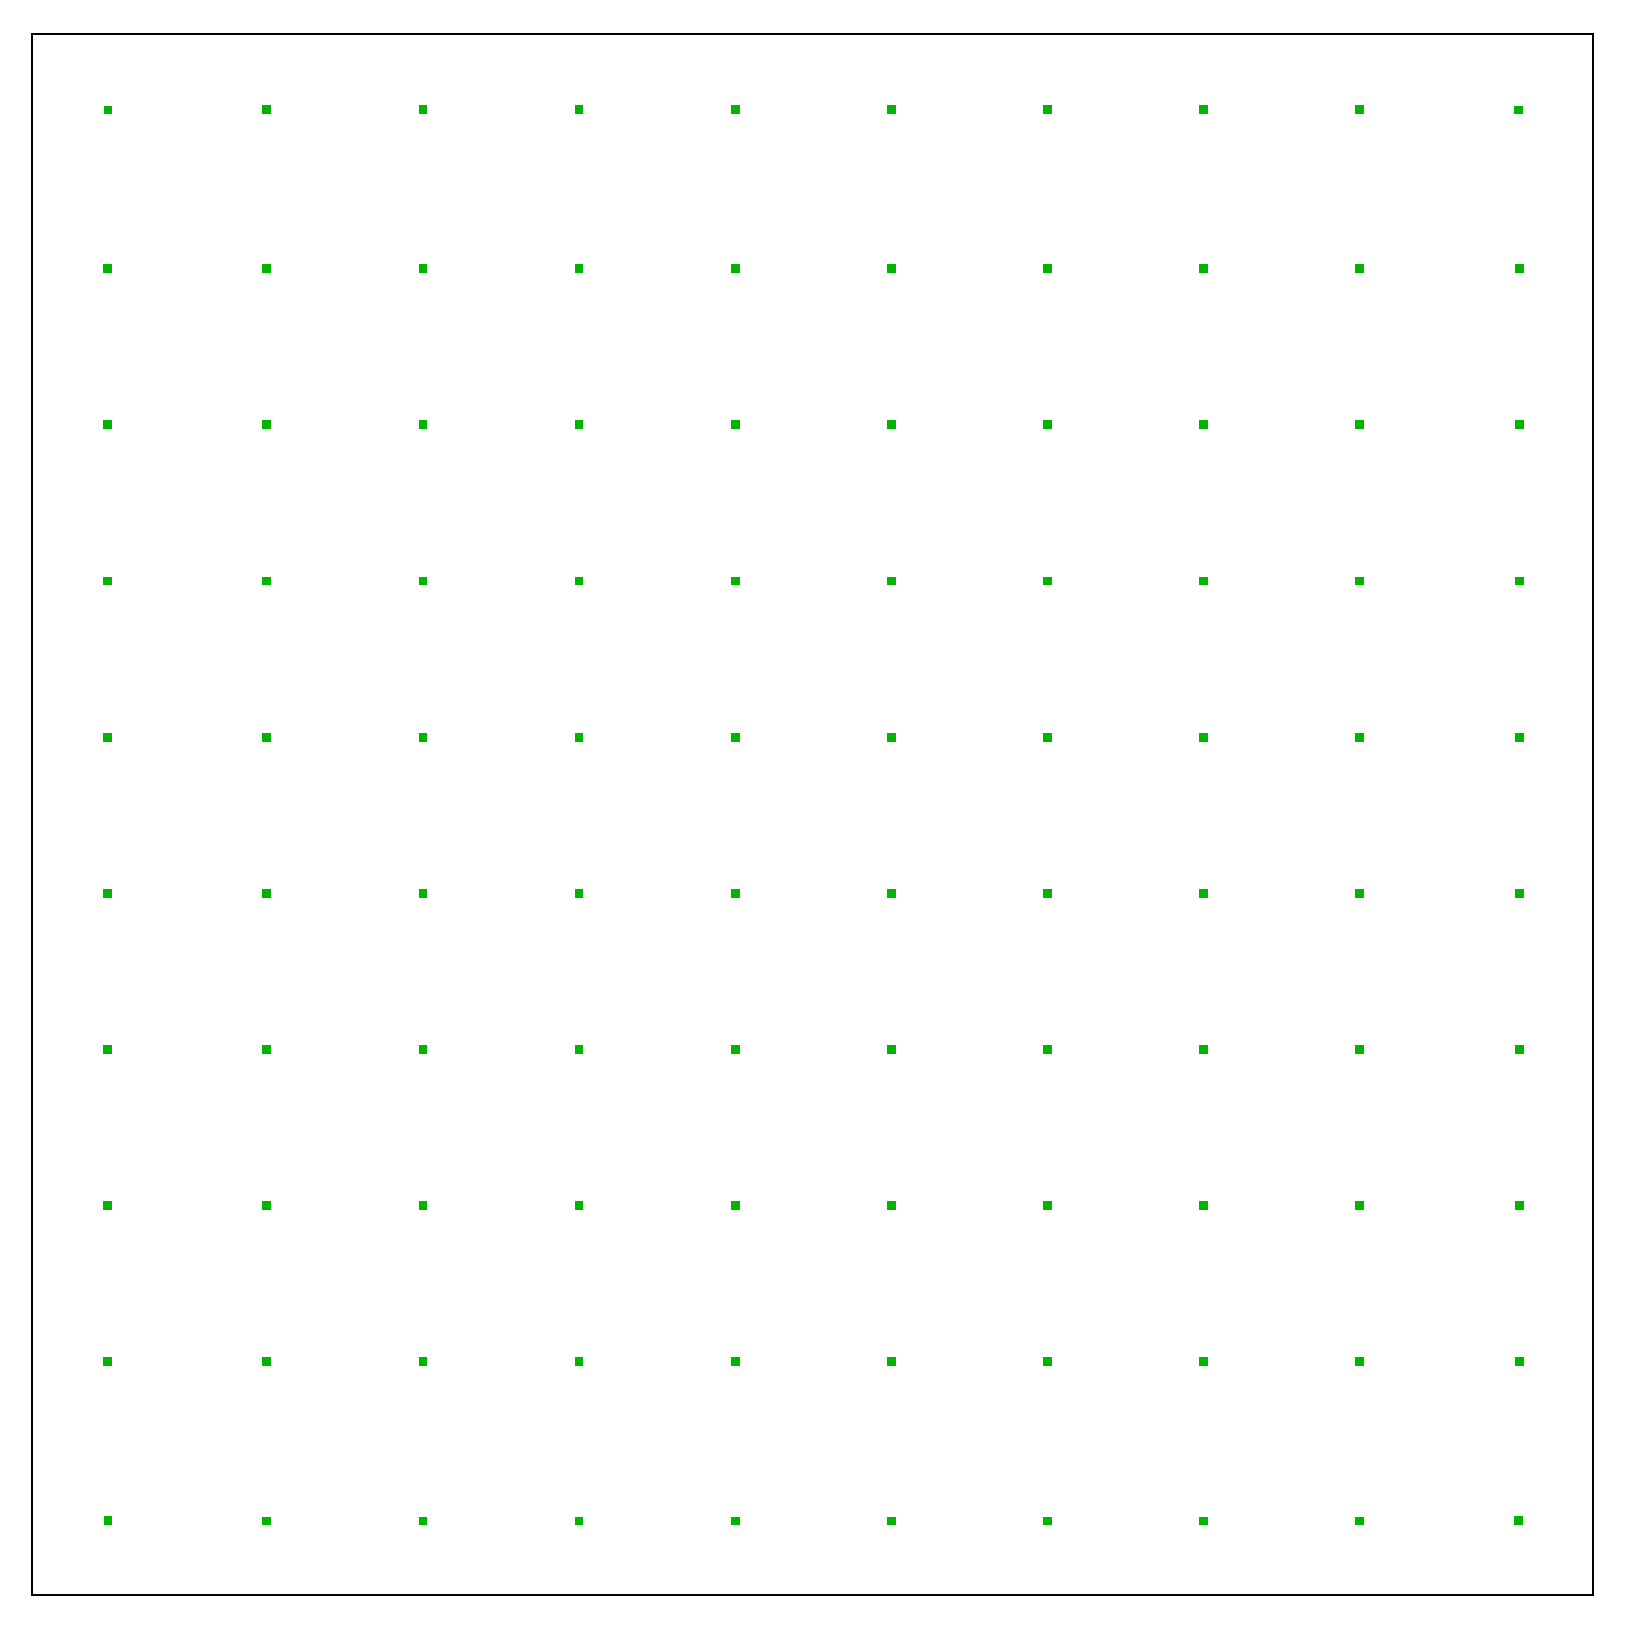
\includegraphics[width=0.33\textwidth]{img/createmap/nodes-start-grid.eps}}
  \subfloat[Pravideln� m��ka s odchylkou 3]{\label{fig:createmap-noise3}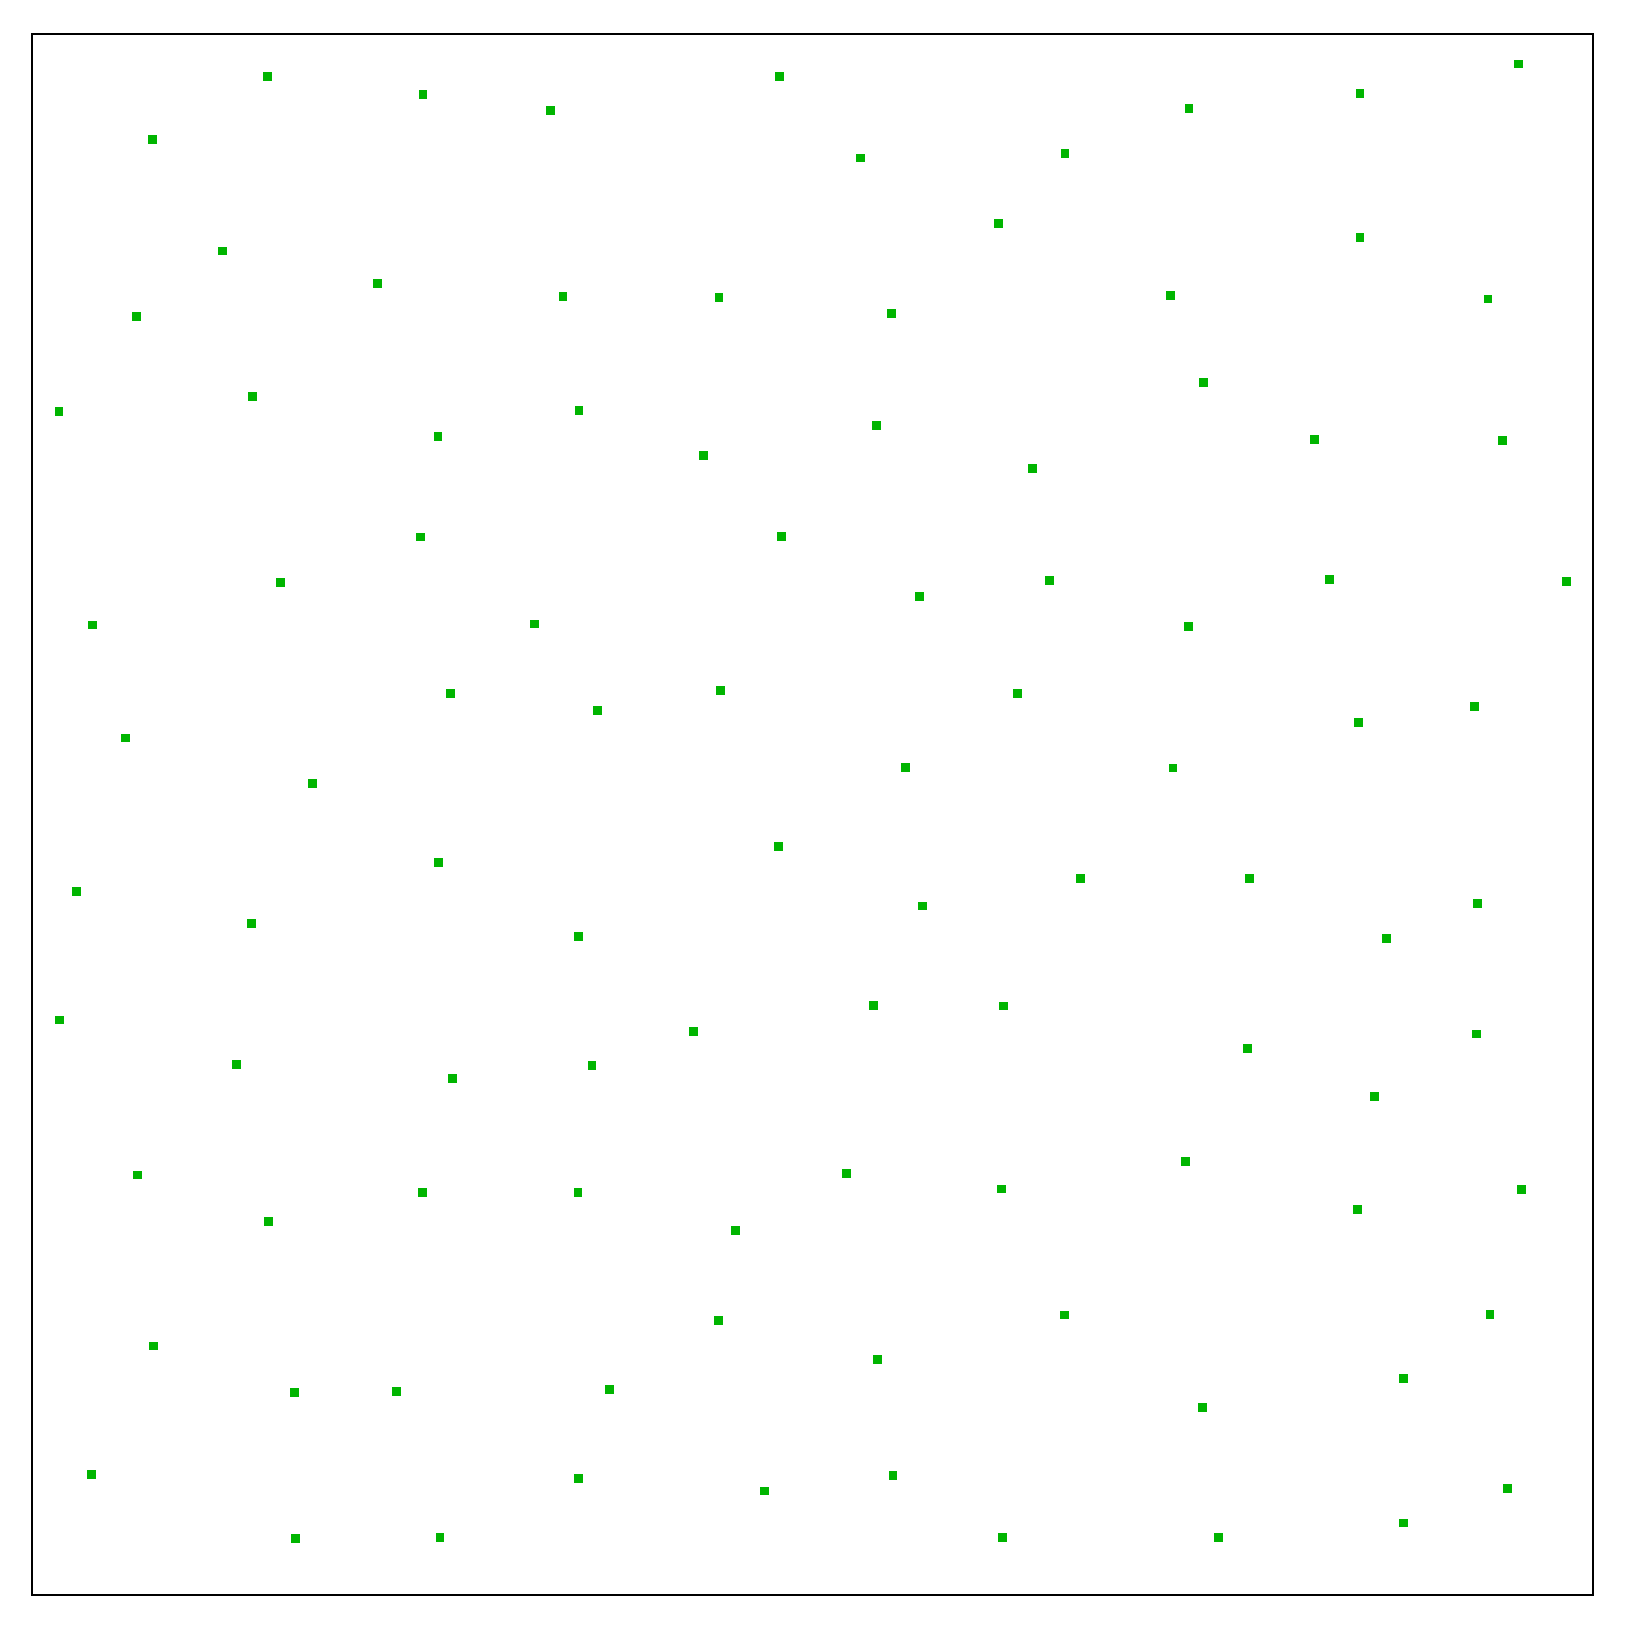
\includegraphics[width=0.33\textwidth]{img/createmap/nodes-start-grid-noise-3.eps}}
  \subfloat[Zcela n�hodn�]{\label{fig:createmap-random}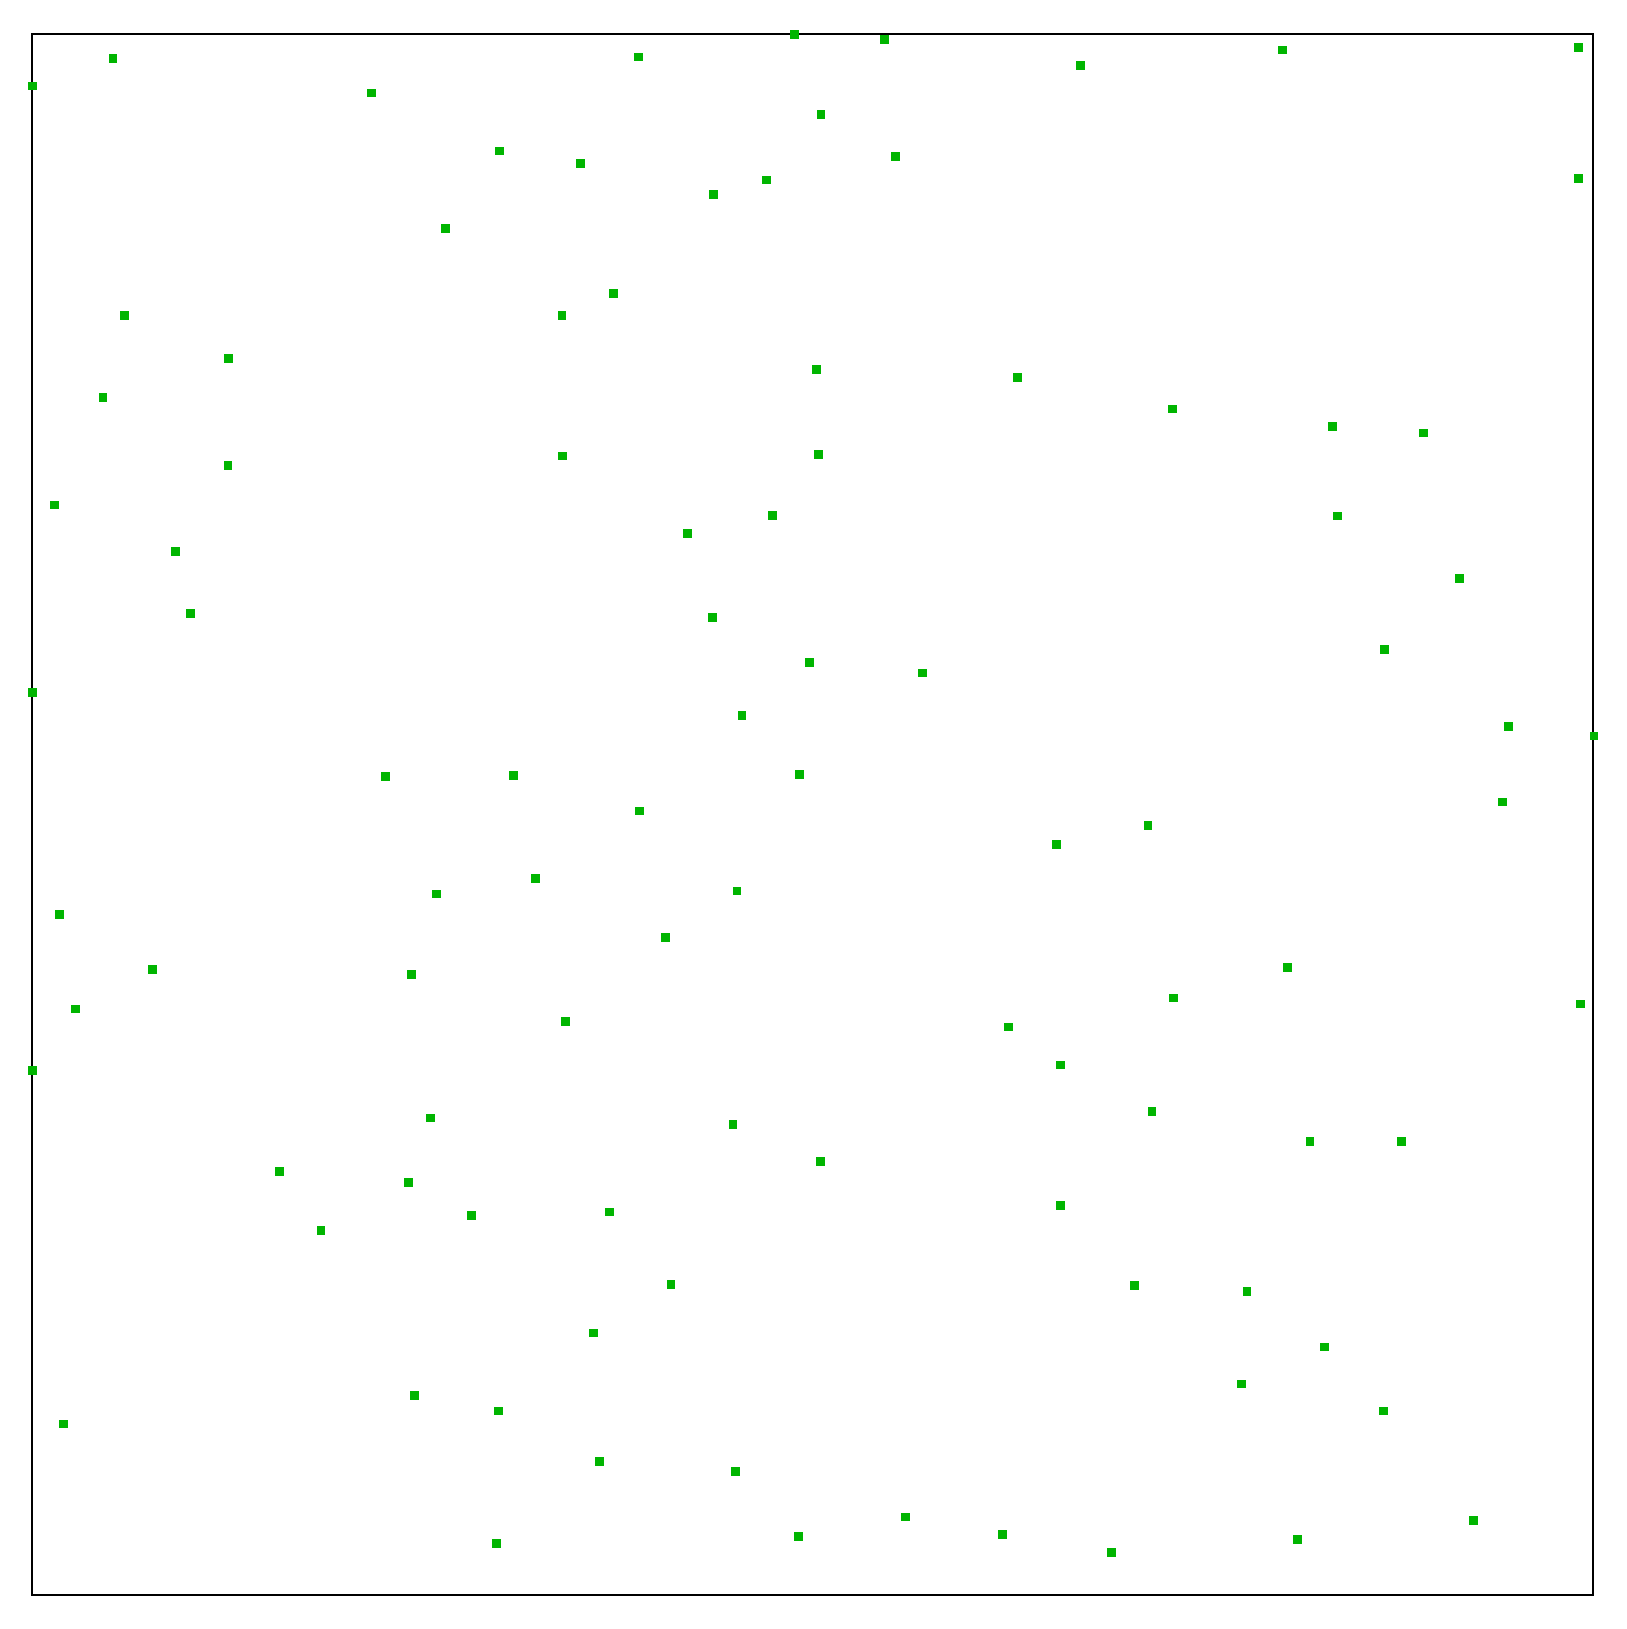
\includegraphics[width=0.33\textwidth]{img/createmap/nodes-start-random.eps}}
  \caption{Po��te�n� rozlo�en� uzl�. Dal�� uk�zky jsou na p�ilo�en�m CD v adres��i ??}
  \label{fig:createmap}
\end{figure}

\begin{definition}[Hustota mapy]
Po�et uzl�, kter� jsou do m�stnosti um�st�ny p�i vytv��en� mapy je ur�en pouze na z�klad� jej� velikosti a hustoty mapy.
Pokud je po��te�n� rozlo�en� mapy pravideln� m��ka, hustota mapy ur�uje, jak daleko od sebe maj� dva uzly b�t.
Jeden uzel pak pokr�v� oblast velikosti �tverce hustoty.
Pokud je rozlo�en� uzl� zcela n�hodn�, je z hustoty mapy odvozen po�et uzl� dle vzorce \eqref{formula:el-start-pocet-uzlu},
kde $obsah(mistnost)$ je obsah polygonu reprezentuj�c� m�stnost a $hustota$ je hustota mapy.
\end{definition}

\begin{equation} 
pocet = \frac{obsah(mistnost)}{hustota^2}
\label{formula:el-start-pocet-uzlu}
\end{equation}
\\



% STOPA VJEMU %%%%%%%%%%%%%%%%%%%%%%%%%%%%%%%%%%%%%%%%%%%%%%%%%%%%%%%%%%%%%%%%%%%%%%%%%%%%%%%%%%%%%%%%%%%%%%%%%%%%%%%%%%%%%%%%%%%%%%%%%%%


\subsection{Stopa vjemu}

Gravita�n� model se u�� z vjem� postupn�.
K tomu vyu��v� tzv. \emph{stopy vjemu}.
P�edstavuj� ur�itou m�ru pozornosti, kterou agent v�nuje jednomu p�edm�tu, kr�tkodob� ulo�en� vjem, kter� chv�li trv� a prostorovou mapu postupn� m�n�.
\\

\begin{definition}[Stopa vjemu]
Kdy� je v ur�it�m kroku simulace prostorov� map� p�ed�n vjem ke zpracov�n�, mapa si jej ulo�� a u�� se dle n�j nekolik dal��ch krok� simulace.
Takto ulo�en� vjem budeme naz�vat stopou vjemu.
Stopa vjemu je dvojice \emph{$<$pam�ov� stopa, intenzita$>$}, kde \emph{pam�ov� stopa}, je pam�ov� stopa p�edm�tu, kter� vjem vyvolal.
Intenzita stopy vjemu je p�i jej�m vytvo�en� odvozena z intenzity vjemu a v pr�b�hu �asu kles�.
Intenzita ur�uje m�ru, s jakou bude stopa vjemu ovliv�ovat prostorovou mapu.
\end{definition}

\begin{definition}[Vliv vjemu]
P�i vytvo�en� stopy vjemu je ur�ena jej� intenzita. Ta z�vis� na intenzit� p�vodn�ho vjemu a tzv. vlivu vjemu.
To je parametr modelu, kter� ovliv�uje rychlost u�en� prostorov� mapy. Budeme jej d�le zna�it $\eta_0$.
(EPCreateEnergy)
\end{definition}

Stopa vjemu postupn� sl�bne. Typicky b�hem n�kolika krok� simulace klesne jej� intenzita z po��te�n� hodnoty bl�zko k nule.
Sl�bnut� stopy z�vis� na dvou parametrech: \emph{m��e sl�bnut�} a \emph{limitu zmizen�}.

\begin{definition}[M�ra slabnut�]
M�ra sl�bnut� ur�uje rychlost kles�n� intenzity. Ovliv�uje, jak dlouho je stopa vjemu ulo�ena.
(EPFadeCoef)
\end{definition}

\begin{definition}[Limit zmizen�]
Stopa vjemu zmiz�, pokud jej� intenzita klesne pod ur�itou hranici - limit zmizen�.
(EPFadeLimit)
\end{definition}

Zpracov�n� p��choz�ho vjemu je tedy pouze vytvo�en� stopy vjemu s odkazem na pam�ovou stopu.
Pokud v dan�m m�st� ji� stopa vjemu je, jej� intenzita je zv��ena. Po��te�n� intenzita stopy resp. zv��en� intenzity je d�no vzorcem:

\begin{equation} 
\eta(stopa) = \eta_0 \times \eta(vjem)
\label{formula:el-stopa-start-int}
\end{equation}


\begin{definition}[Dosah p�ita�livosti]
Parametr modelu dosah p�ita�livosti ur�uje, na jakou vzd�lenost jsou p�itahov�ny uzly mapy k stop�m vjemu. Vzd�len�j�� uzly nejsou p�itahov�ny.
(ELGravityRange)
\end{definition}

Jeden krok simulace stopy vjemu je pops�n v algoritmu \ref{alg:stopa-step}. V jeho prvn�m kroku je zkonstruov�na mno�ina okoln�ch uzl�:

\begin{equation} 
nodes_{around} = \{ n \in nodes ; dist(n, stopa) < dosah_{pritazlivost} \}
\label{formula:el-okolni-uzly-g}
\end{equation}


\begin{algorithm}[h!]
\caption{Jeden krok simulace pro stopu vjemu}
\label{alg:stopa-step}
\begin{algorithmic}[1]
\State $nodes_{around} \gets$ v�echny uzly v okol� stopy
\ForAll{$node \in nodes_{around}$}
	\State $node_{xy} \gets node_{xy} + \Delta_{xy}$ dle vzorce \eqref{formula:el-ep-gravitace} \label{alg:ep-step-gravitace}
\EndFor
\ForAll{$node \in nodes_{around}$}
	\State $\Delta \eta \gets \eta(node, bod)$ dle vzorce \eqref{formula:el-intenzita} \label{alg:ep-step-intenzita}
	\State zv��en� intenzity vazby mezi $node$ a pam�ovou stopou p�edm�tu o $\Delta \eta$
\EndFor
\State $\eta(stopa) \gets \eta(stopa) \times$ EPFadeCoef
\If{$\eta(stopa) <$ EPFadeLimit}
	\State zmizen� stopy vjemu
\EndIf
\end{algorithmic}
\end{algorithm}


Na ��dku \ref{alg:ep-step-intenzita} je zv��ena intenzita vazby mezi uzlem a pam�ovou stopu.
Zv��en� je d�no podobn�m vzorcem jako \eqref{formula:intenzita-vazby} s jedin�m rozd�lem, �e m�sto vjemu se pracuje s jeho stopou:

\begin{equation} 
\Delta \eta(node, bod) = \eta(stopa) \times \frac{ norm( dist(node, stopa) ) }
{\sum_{n \in nodes_{around}}
  norm( dist(n, stopa) )
}
\label{formula:el-intenzita}
\end{equation}
\\

kde $nodes_{around}$ je mno�ina v�ech uzl� v okol� stopy vjemu.
Funkce $norm$ je libovoln� klesaj�c� funkce maj�c� obor hodnot $<0,1>$, nap�. nep��m� �m�ra $norm(x) = 1/max(1,x)$ �i Gaussova funkce.
\\

Na ��dku \ref{alg:ep-step-gravitace} je pou�ita zm�na polohy uzlu $\Delta_{xy}$, je d�na vzorcem:

\begin{equation} 
\Delta_{xy}(node, stopa) = \frac{\eta(stopa)}{\eta_0} \times \frac{ sila_{pritazlivost} }{ dist(node, stopa)^2 \times \mu(node) }
\label{formula:el-ep-gravitace}
\end{equation}
\\


% ODPUDIVOST UZLU %%%%%%%%%%%%%%%%%%%%%%%%%%%%%%%%%%%%%%%%%%%%%%%%%%%%%%%%%%%%%%%%%%%%%%%%%%%%%%%%%%%%%%%%%%%%%%%%%%%%%%%%%%%%%%%%%%%%%%%%%%%

\subsection{Odpudivost uzl�}

V ka�d�m kroku simulace se uzly, kter� jsou p��li� bl�zko u sebe, odpuzuj�.

\begin{definition}[Dosah odpudivosti]
Parametr modelu dosah odpudivosti ur�uje, na jakou vzd�lenost se uzly mapy je�t� odpuzuj�. Vzd�len�j�� uzly se neodpuzuj�.
(ELAntigravityRange)
\end{definition}

\begin{definition}[S�la odpudivosti]
Parametr modelu s�la odudivosti ur�uje, jak moc se uzly mapy odpuzuj�. P�sob� jako opak s�ly p�ita�livosti.
(ELAntigravityRange)
\end{definition}

\begin{definition}[Vliv napln�nosti]
Parametr modelu vliv napln�nosti ur�uje, jak velk� vliv m� napln�nost uzlu na jeho odpudivost s ostatn�mi uzly.
(ELAGUsageCoef)
\end{definition}

\begin{definition}[Limit pohybu]
Parametr modelu limit pohybu ur�uje maxim�ln� mo�nou zm�nu polohy uzlu v jednom kroku simulace.
(MaxELNodeMove)
\end{definition}

Zm�na polohy uzlu kv�li odpudivosti je sou�et odpudiv�ch sil okoln�ch uzl� a je nep��mo �m�rn� napln�nosti uzlu.
Nejd��ve jsou ur�eny okoln� uzly jako mno�ina:

\begin{equation} 
nodes_{around} = \{ n \in nodes ; dist(n, stopa) < dosah_{odpudivost} \}
\label{formula:el-okolni-uzly-ag}
\end{equation}


Pro v�echny okoln� uzly je spo�tena vz�jemn� odpudivost dle vzorce:

\begin{equation} 
odpudivost(n_i, n_j) = \frac{ sila_{odpudivost} }{ dist'(n_i, n_j)^2 \times \mu'(n_i) \times \mu'(n_j) } 
\label{formula:el-odpudivost}
\end{equation}

kde

\begin{equation} 
dist'(a,b) = max(1,dist(a,b))
\end{equation}

a

\begin{equation} 
\mu'(node) = max(\mu_{vliv},\mu'(node))
\end{equation}
 
Funkce $max$ jsou pou�ity, aby zabr�nily d�len� nulou a sn�ily vliv vzd�lenosti a napln�nosti na odpudivost uzl�.
\\

Po ur�en� v�ech odpudiv�ch sil, kter� na uzly p�sob�, jsou polohy uzl� upraveny dle t�chto sil a jejich aktu�ln� napln�nosti:

\begin{equation} 
\Delta_{xy}(node) = \frac{
\sum_{\substack{
   n \in nodes
  }}
  odpudivost(n, node)
}{ max(1, \mu(node)) } 
\label{formula:el-odpudivost}
\end{equation}
\\

Funkce $max$ je ve vzorci op�t pou�ita, aby zabr�nila d�len� nulou a p��li� velk�m zm�n�m polohy uzl� pro $\mu(node) \to 0$.
P�esto je mo�n�, �e se v jednom kroku simulace nas��taj� takov� odpudiv� a p�ita�liv� s�ly, �e by zm�na polohy uzlu mohla p�es�hnout rozumnou mez.
Nechceme, aby kv�li kr�tkodob�m stav�m s�t� \footnote{nap�. p�i vytvo�en� nov�ho uzlu prostorov� mapy} uzly p��li� m�nily svou polohu.
P�idali jsme tedy omezen� na maxim�ln� mo�n� pohyb uzlu - parametr modelu \param{limit pohybu}.


Alternativn� �e�en� by bylo zmen�it parametr \param{s�la odpudivosti} a \param{s�la p�ita�livosti} a prov�st v�ce krok� simulace.
To je v�ak velmi n�ro�n� na v�kon a v��e uveden� �e�en� toto vlastn� imituje.
\\

\subsection{Omezen� pohybu uzl�}
N�sledkem odpudivosti uzl� je mo�n�, �e se model bude sna�it p�esunout uzel mimo sv�t, resp. vn� polygonu sv�t reprezentuj�c�.
V tom p��pad� je uzel na okraj sv�ta, tj. na hranu polygonu v m�st� jej�ho pr�se��ku s �se�kou p�edstavuj�c� pl�novanou trajektori� uzlu.
Pokud se v dal��ch kroc�ch simulace bude model op�t sna�it p�esunout uzel vn� polygonu, bude jeho trajektorie prom�tnuta na hranu polygonu, na kter� uzel le��.
Uzel tak bude "klouzat" po hran� polygonu, jak je uk�z�no na obr�zku \ref{fig:slide-on-edge}.
\\

\begin{figure}[h]
  \centering
  \scalebox{0.8}{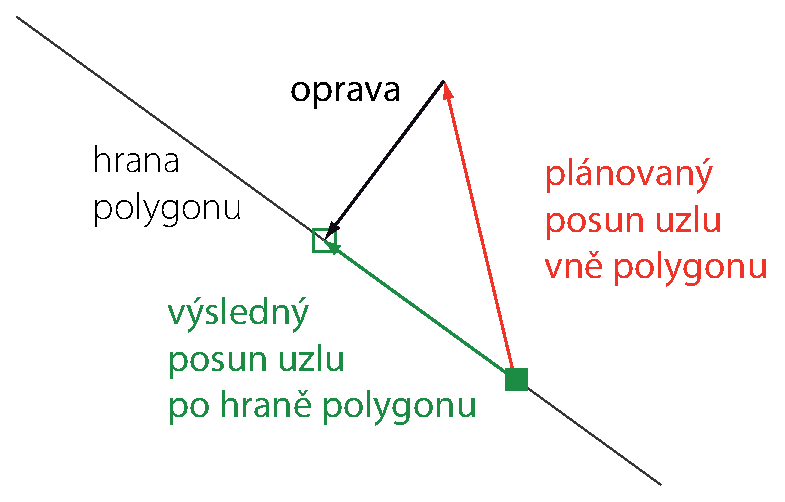
\includegraphics{img/slide-on-edge.ps}}
  \caption{Zm�na posunu uzlu, kdy� naraz� na hranu polygonu}
  \label{fig:slide-on-edge}
\end{figure}





% ZMENA POCTU UZLU %%%%%%%%%%%%%%%%%%%%%%%%%%%%%%%%%%%%%%%%%%%%%%%%%%%%%%%%%%%%%%%%%%%%%%%%%%%%%%%%%%%%%%%%%%%%%%%%%%%%%%%%%%%%%%%%%%%%%%%%%%%

\subsection{Zm�na po�tu uzl�}

Je ��douc�, aby se po�et uzl� prostorov� mapy v pr�b�hu simulace m�nil, dle po�tu p�edm�t�, kter� agent vid�l resp. dle �etnosti a intenzity vjem�.
Mapa tedy vytv��� nov� uzly a zapom�n� existuj�c� uzly. 
Nov� uzly vytv��� stopy vjemu na z�klad� jejich intenzity.
Zapom�n�n� uzl� se d�je v ka�d�m kroku simulace resp. v ka�d�m kroku simulace je ur�it� pravd�podobnost, �e dojde k zapomenut� uzlu.
\\

\begin{definition}[Cena vytvo�en� uzlu]
Vytvo�en� nov�ho uzlu stoj� ur�it� mno�stv� intenzity stopy vjemu. Toto mno�stv� budeme naz�vat cena vytvo�en� uzlu a d�le jej budeme zna�it $cost_{create}$.
\end{definition}

\begin{definition}[Odchylka vytvo�en� uzlu]
Parametr modelu \param{odchylka vytvo�en� uzlu} ur�uje, jak daleko od stopy vjemu m��e b�t nov� uzel vytvo�en.
Pokud bude roven nule, budou v�echny uzly vytv��eny p�esn� v poloze stopy vjemu. To by vedlo k d��ve uveden�m probl�m�m s vysokou odpudivost�.
(ELNodeAddNoise)
\end{definition}

\begin{definition}[Po��te�n� napln�nost uzlu]
Parametr modelu, ur�uj�c� po��te�n� napln�nost uzlu. ??
(MemObjIntenseToNewNode)
\end{definition}

Roz���ili jsme jeden krok simulace pro stopu vjemu - algoritmus \ref{alg:stopa-step} - o vytv��en� nov�ch uzl�, algoritmus \ref{alg:stopa-step-create}.

\begin{algorithm}[h!]
\caption{Vytv��en� uzl� v r�mci stopy vjemu}
\label{alg:stopa-step-create}
\begin{algorithmic}[1]
\State $p_{create} \gets$ pravd�podobnost vzniku nov�ho uzlu dan� vzorcem \eqref{formula:el-pst-node-create} \label{alg:ep-step-create}
\State $r \gets$ n�hodn� ��slo $r \in <0,1>$
\If{$r < p_{create}$}
  \State vytvo�en� nov�ho uzlu
  \State vytvo�en� vazby uzlu na pam�ovou stopu bodu energie
  \State $\eta(stopa) \gets \eta(stopa) - cost_{create}$ \label{alg:ep-step-cost}
\EndIf
\end{algorithmic}
\end{algorithm}


Na ��dku \ref{alg:ep-step-create} je pou�ita pravd�podobnost vytvo�en� nov�ho uzlu, ta je d�na vzorcem:
\begin{equation} 
p_{create}(\eta(stopa), cost_{create}) = \frac{\eta(stopa) - cost_{create}}{cost_{create}}
\label{formula:el-pst-node-create}
\end{equation}
\\

Nov� vytvo�en� uzel bude m�t stejnou polohu jako stopa vjemu s n�hodnou odchylkou \(\in <-\Delta,\Delta>\), kde $\Delta$ je \param{odchylka vytvo�en� uzlu}.
Jeho napln�nost bude \param{po��te�n� napln�nost uzlu}.
\\


\begin{definition}[Cena zapomenut� uzlu]
Zapomenut� uzlu stoj� ur�it� mno�stv� energii na zapom�n�n�. Toto mno�stv� budeme naz�vat cena zapomenut� uzlu a d�le jej budeme zna�it $cost_{forget}$.
\end{definition}

\begin{definition}[M�ra zapom�n�n� uzl�]
Parametr modelu \param{m�ra zapom�n�n� uzl�} ur�uje jak rychle bude prostorov� mapa zapom�nat uzly.
(ELForgetNodeRate)
\end{definition}

K zapomenut� m��e doj�t ka�d� kroku simulace. Vrstva uzl� akumuluje tzv. energii na zapom�n�n� $e_{forget}$.
Na za��tku je rovn� nule a v pr�b�hu simulace roste.
V ka�d�m kroku je zv��ena o hodnotu parametru \param{m�ra zapom�n�n� uzl�}.
D�le je ur�ena pravd�podobnost, �e bude zapomenut uzel $p_{forget}$:

\begin{equation} 
p_{forget} = \frac{e_{forget} - cost_{delete}}{cost_{forget}}
\label{formula:el-pst-forget}
\end{equation}

Pokud m� doj�t k zapomenut� uzlu, je vybr�n n�hodn� uzel a ten je odstran�n z prostorov� mapy v�etn� v�ech jeho vazeb na pam�ov� stopy.
Proces zapom�n�n� uzlu je pops�n algoritmem \ref{alg:node-forget}.

\begin{algorithm}[h!]
\caption{Zapom�n�n� uzl�}
\label{alg:node-forget}
\begin{algorithmic}[1]
\State $e_{forget} \gets e_{forget} + rate_{forget}$
\State $p_{forget} \gets$ pravd�podobnost zapomenut� uzlu dan� vzorcem \eqref{formula:el-pst-forget} \label{alg:el-forget}
\State $r \gets$ n�hodn� ��slo $r \in <0,1>$
\If{$r < p_{forget}$}
  \State $node \gets $ n�hodn� vybran� uzel
  \State $e_{forget} \gets e_{forget} - cost_{forget} \times norm(\mu(node)) $ \label{alg:el-forget-cost}
  \State zapomenut� uzlu
\EndIf
\end{algorithmic}
\end{algorithm}


Kdy� je z mapy odstran�n uzel, m��e doj�t a typicky doch�z� k naru�en� nau�en�ho rovnom�rn�ho rozlo�en� uzl� v prostoru, smazan� uzel za sebou nech�v� pr�zdn� m�sto.
��st prostorov� mapy kolem smazan�ho uzlu by bylo vhodn� p�eu�it, p�emistit uzly, aby byly op�t rovnom�rn� rozd�len�.
Proto je p�i smaz�n� uzlu provedeno n�kolik lok�ln�ch krok� simulace, kdy je prov�d�no pouze odpuzov�n� uzl� v okol� smazan�ho uzlu.
Tento proces m� dva parametry: \param{po�et opakov�n�} a \param{velikost okol�}.
\\

\begin{definition}[Po�et opakov�n�]
Parametr modelu \param{po�et opakov�n�} ur�uje po�et opakov�n� lok�ln�ch krok� simulace.
(ELDeleteNodeReTrainCount)
\end{definition}

\begin{definition}[Velikost okol�]
Parametr modelu \param{velikost okol�} ur�uje velikost okol�, tj. uzly, jejich� poloha se m�n�.
(ELDeleteNodeReTrainRange)
\end{definition}


V��e uvedenou cenu vytvo�en� a zapomenut� uzlu m��eme ur�it mnoha zp�soby.
Prvn� mo�nost� je konstantn� cena v pr�b�hu simulace.


\begin{figure}[h!]
  \centering
  \subfloat[EmptyRoom]{\label{fig:nc-100-empty}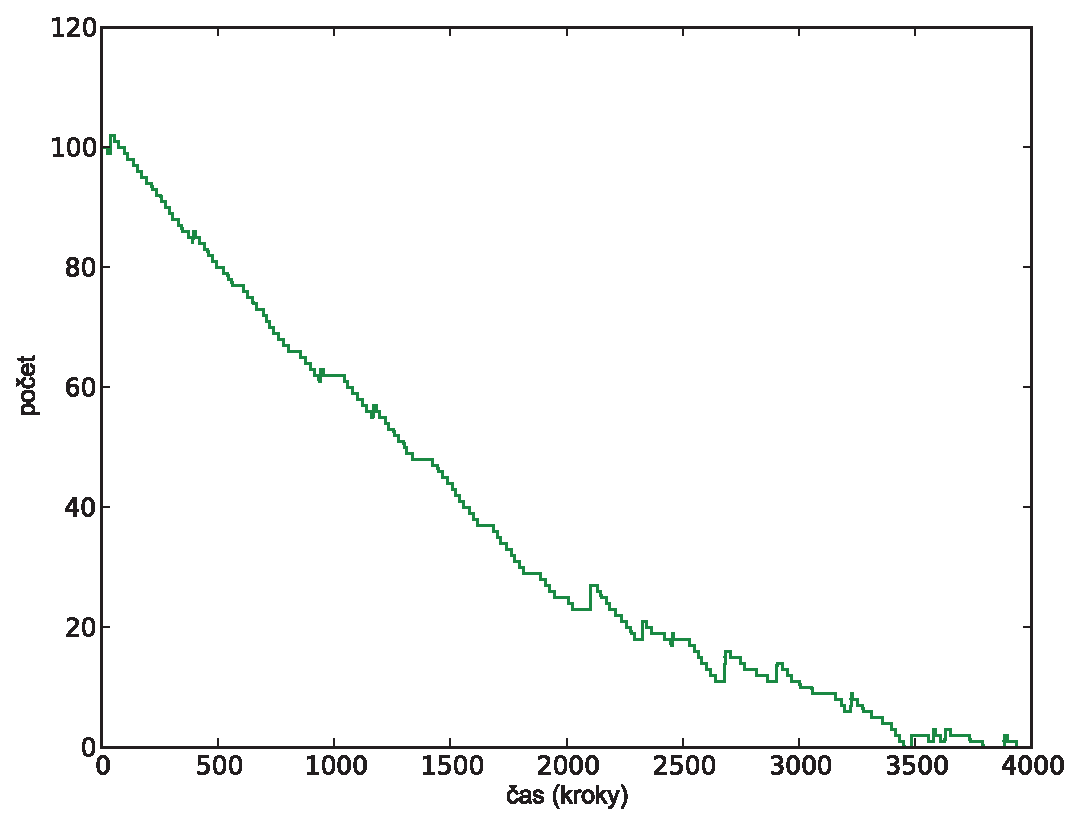
\includegraphics[width=0.5\textwidth]{img/nc/100-empty.eps}}
  \subfloat[FullRoom]{\label{fig:nc-100-full}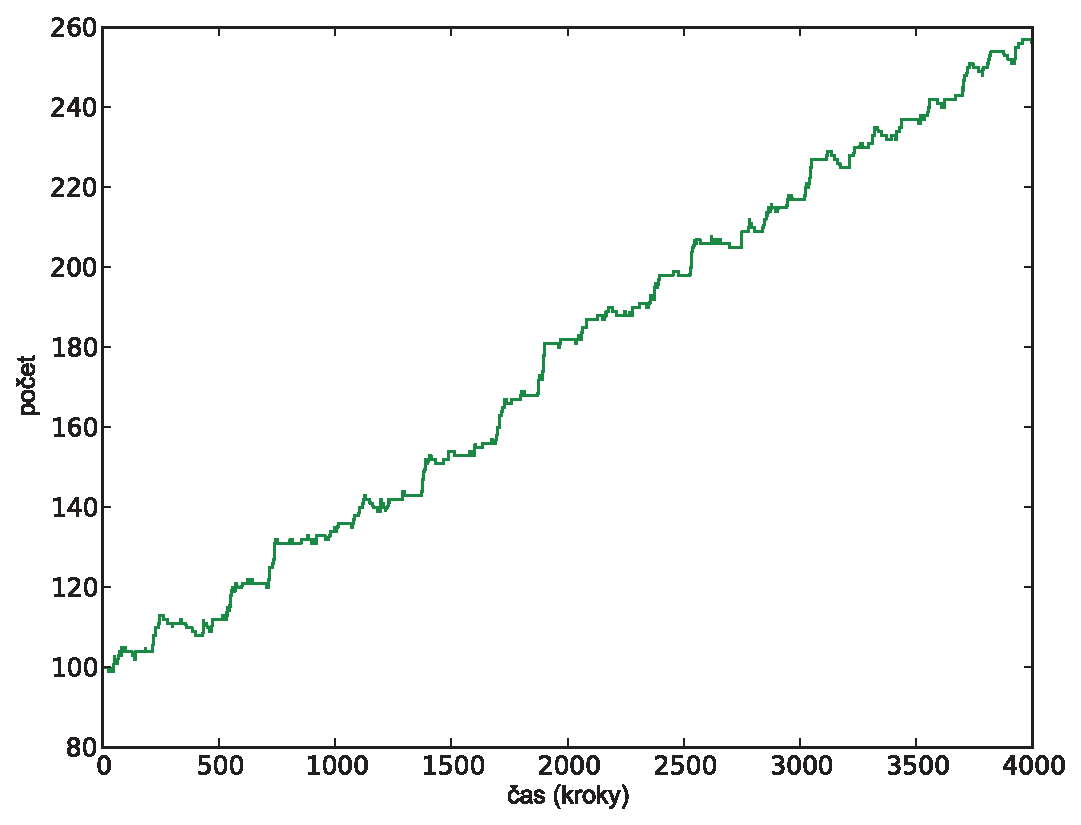
\includegraphics[width=0.5\textwidth]{img/nc/100-full.eps}}
  \caption{Test konstantn� ceny}
  \label{fig:nc-fixed}
\end{figure}

V�sledek testu konstantn� ceny je na obr�zku \ref{fig:nc-fixed}. Graf zobrazuje po�et uzl� prostorov� mapy v �ase.
Na konkr�tn� hodnot� nez�le��, v�sledky s nimo jsou obdobn�\footnote{Jsou na p�ilo�en�m CD}.
Pokud je cena konstantn�, v m�stnost s v�t��m po�tem p�edm�t� uzl� neust�le p�ib�v�. V m�stnosti s mal�m po�tem p�edm�t� uzly miz� a jejich po�et kles� a� k nule.
Je tedy z�ejm�, �e cena nem��e b�t konstatn�.
\\


\begin{definition}[Cht�n� po�et uzl�]
Ze vzorce \eqref{formula:el-start-pocet-uzlu} je ur�en po��te�n� po�et uzl�.
Cht�n� po�et uzl� $n_{desired}$ je po�et uzl�, kter� by v prostoru m�ly b�t, ur�en� jen dle jeho velikosti.
Je to konstanta, dvojn�sobek po�tu uzl�, kter� jsou do prostoru um�st�ny na za��tku.
\end{definition}

Cht�li bychom, aby po�et uzl� mapy se po ur�it� dob� ust�lil a aby tento po�et reflektoval �etnost vjem�.
Definujme cenu vytvo�en� uzlu $cost_{create}$ resp. zapomenut� uzlu $cost_{forget}$ jako funkci $n_{desired}$ a aktu�ln�ho po�tu uzl� $n_{current}$.
Pro jednudochost budou tyto funkce symetrick� dle osy y, $cost_{create}$ bude rostouc� a $cost_{forget}$ klesaj�c�.
\\




Jsou ur�eny vzorcem:

\begin{equation} 
cost_{create}(n_{desired}, n_{current}) = 100 \times 3^{ \frac{n_{diff}}{50} }
\label{formula:cost-create}
\end{equation}

resp.

\begin{equation} 
cost_{delete}(n_{desired}, n_{current}) = 100 \times 3^{ - \frac{n_{diff}}{50} }
\label{formula:cost-delete}
\end{equation}
\\

$n_{diff}$ je prom�nn� vyjad�uj�c� rozd�l mezi aktu�ln�m po�tem a cht�nn�m po�tem uzl� dle vzorce:

\begin{equation} 
n_{diff}(n_{desired}, n_{current}) = NodeCostCoef \times \frac{ n_{current} - n_{desired} }{ n_{desired} }
\label{formula:forget-chance}
\end{equation}
\\

?? OBR grafy funkc� ??
\\




















\subsection{Hiearchie}

Jedn�m z po�adavk� na model vrstvy uzl� je, aby um�l vytv��et hiearchii uzl�. Model mus� b�t schopen rozpoznat m�sta s vy��� hustotou uzl�.
\\

Uzl�m prostorov� mapy p�id�me dal�� vlastnost \emph{AGamount}, mno�stv� odpudivosti, kter� uzel za svoji existenci poc�til.
P�i vytvo�en� uzlu je nastavena na nulu. V ka�d�m kroku p�i po��t�n� odpudiv�ch sil p�sob�c�ch na uzel, je zv��ena o:

\begin{equation} 
\Delta_{AGamount}(node) = \sum_{
 	\substack{
		n \in nodes
	}}
  |odpudivost(n, node)|
\label{formula:el-agamount}
\end{equation}
\\

Mno�stv� odpudivosti v uzlu je sledov�no a kdy� p�ekro�� limit dan� modelem, parametr HLAGNeeded, algoritmus \ref{alg:hl-create} vytvo�� nov� uzel vy��� �rovn�.
\\







\subsection{V�sledn� model}

finalni alogoritmus EP




V ka�d�m kroku simulace je pro ka�dou stopu vjemu proveden algoritmus \ref{alg:ep-step-final}.

\begin{algorithm}[h!]
\caption{Jeden krok simulace pro bod energie}
\label{alg:ep-step-final}
\begin{algorithmic}[1]
\State $p_{create} \gets$ pravd�podobnost vzniku nov�ho uzlu dan� vzorcem \eqref{formula:el-pst-node-create} \label{alg:ep-step-create}
\State $r \gets$ n�hodn� ��slo $r \in <0,1>$
\If{$r < p_{create}$}
	\State vytvo�en� nov�ho uzlu
	\State vytvo�en� vazby uzlu na pam�ovou stopu bodu energie
	\State $bod_{energy} \gets bod_{energy} - cost_{create}$ \label{alg:ep-step-cost}
\EndIf
\State $nodes \gets$ v�echny uzly v okol� bodu energie
\ForAll{$node \in nodes$}
	\State $node_{xy} \gets node_{xy} + \Delta_{xy}$ dle vzorce \eqref{formula:el-ep-gravitace} \label{alg:ep-step-gravitace}
\EndFor
\ForAll{$node \in nodes$}
	\State $\Delta \eta \gets \eta(node, bod)$ dle vzorce \eqref{formula:el-intenzita} \label{alg:ep-step-intenzita}
	\State zv��en� intenzity vazby mezi $node$ a pam�ovou stopou bodu o $\Delta \eta$
\EndFor
\State $bod_{energy} \gets bod_{energy} \times$ EPFadeCoef
\If{$bod_{energy} <$ EPFadeLimit}
	\State zru�en� bodu energie
\EndIf
\end{algorithmic}
\end{algorithm}




\subsection{Slo�itost algoritm�}




\chapter{V�sledky test� modelu}

Tato kapitola obsahuje v�sledky test� modelu.
Jednak testy fin�ln�ho modelu na r�zn�ch datech, druhak testy modelu s r�zn�mi hodnotami n�kter�ch kl��ov�ch parametr�.
\\

Samotn� test je ur�en testovac�m sv�tem\footnote{P�ehled v�ech testovac�ch m�stnost� je v p��loze A.}
, tedy m�stnost� a sc�n��em a hodnotami parametr�.
V n�kter�ch p��padech bylo testov�na r�zn� �e�en� konkr�tn�ch pod�loh.
V takov�ch p��padech nesta�� zm�nit parametry modelu, ale je nutn� upravit samotn� algortimus.
Takov� p��pady budou explicitn� pops�ny a r�zn� algoritmy vysv�tleny.
\\



 obr�zek ukazuj�c� stav sv�ta a prsotorov� mapy v 

\section{Testy fin�ln�ho modelu}

Test vysledneho modelu - vsechna data a vetsina mistnosti
Vse pak mit na CD
\\


\section{Vliv napln�nosti} \label{chapter-test-ag}

V tomto testu uk�eme, jak d�le�itou roli hraje vliv napln�nosti p�i ur�ov�n� vz�jemn� odpudivosti dvou uzl� ve vzorci \eqref{formula:el-odpudivost}.
Provedli jsme 5000 krok� simulace v m�stnostech EmptyRoom a FullRoom. ?? adresar na CD ??.
\\

V prvn�m testu nebyla napln�nost uzl� p�i po��t�n� odpudivosti v�bec br�na v �vahu.
V�sledek je na obr�zku \ref{fig:usage-ag-no} a ukazuje, �e v tom p��pad� model rozmis�uje uzly v prostoru t�m�� rovnom�rn�.
Z toho vypl�v�, �e napl�nost uzlu hraje v modelu v�znamnou roli.
Obr�zky \ref{fig:usage-ag-0.5}, \ref{fig:usage-ag-0.8}, \ref{fig:usage-ag-1} ukazuj� v�sledky test� pro r�zn� hodnoty \param{vlivu napln�nosti}.
\\

\begin{figure}[p]
  \centering
  \subfloat[EmptyRoom]{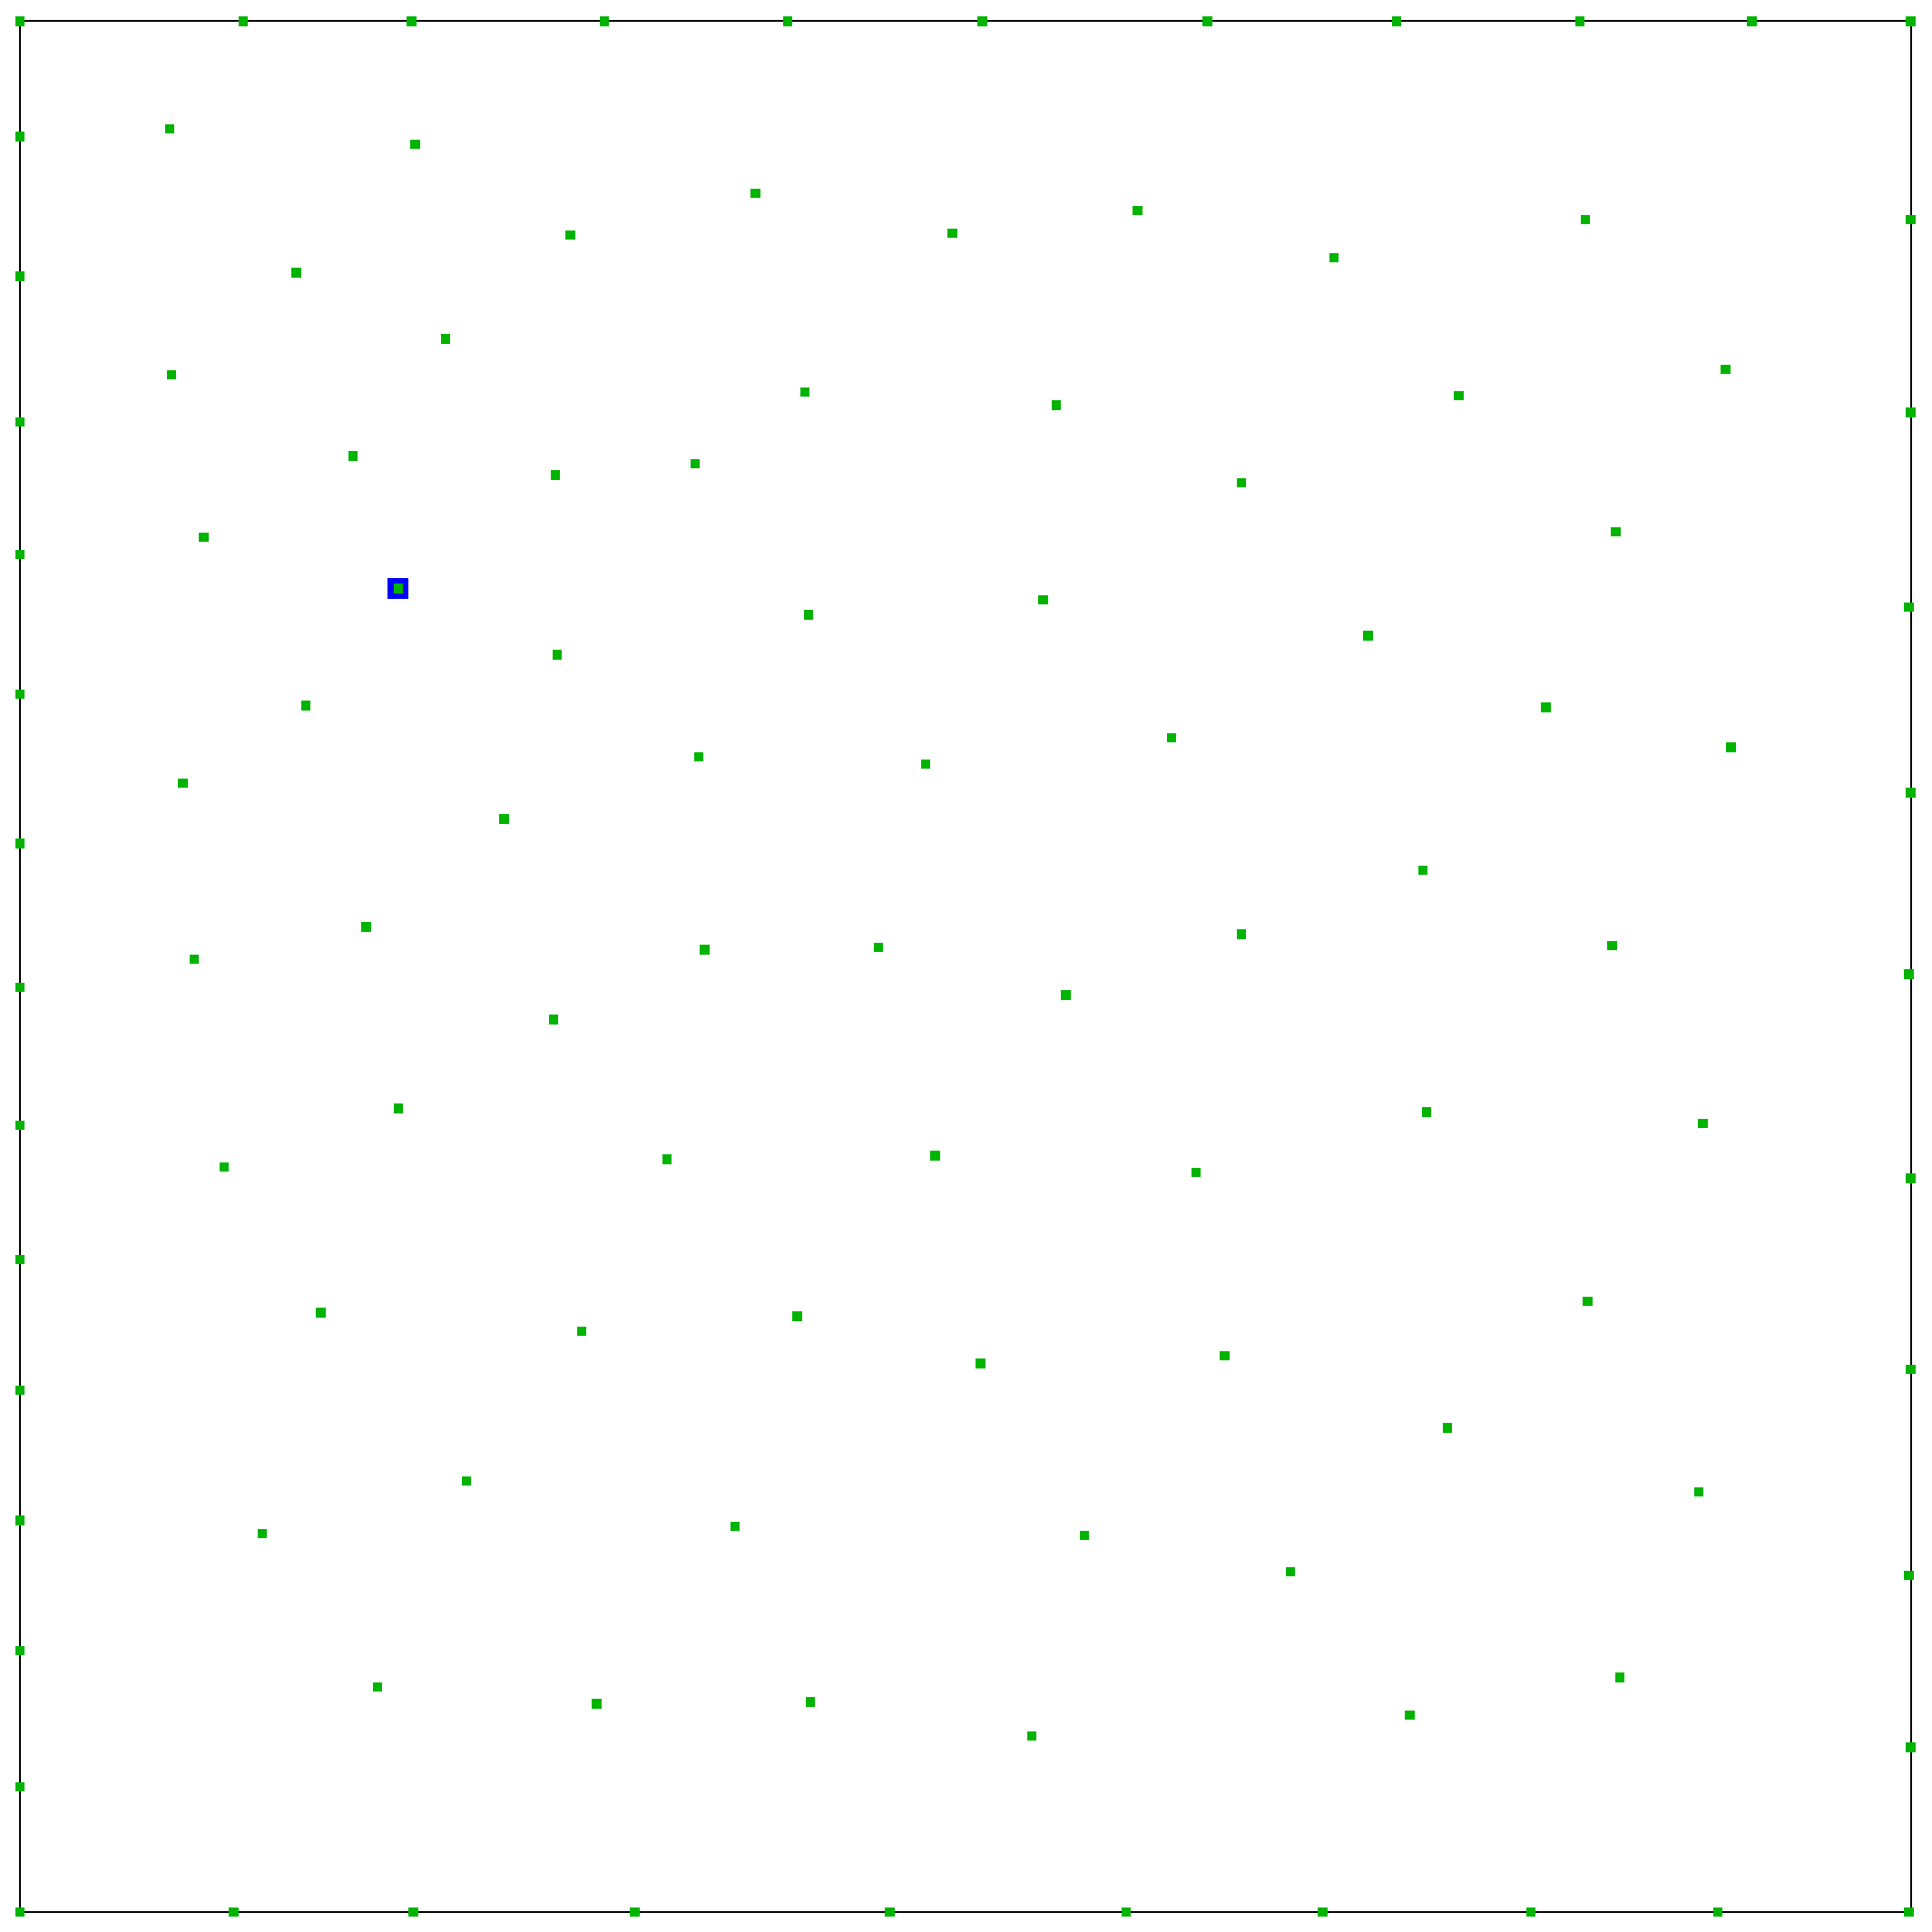
\includegraphics[width=0.5\textwidth]{img/usage/nousage-empty.eps}}
  \subfloat[FullRoom]{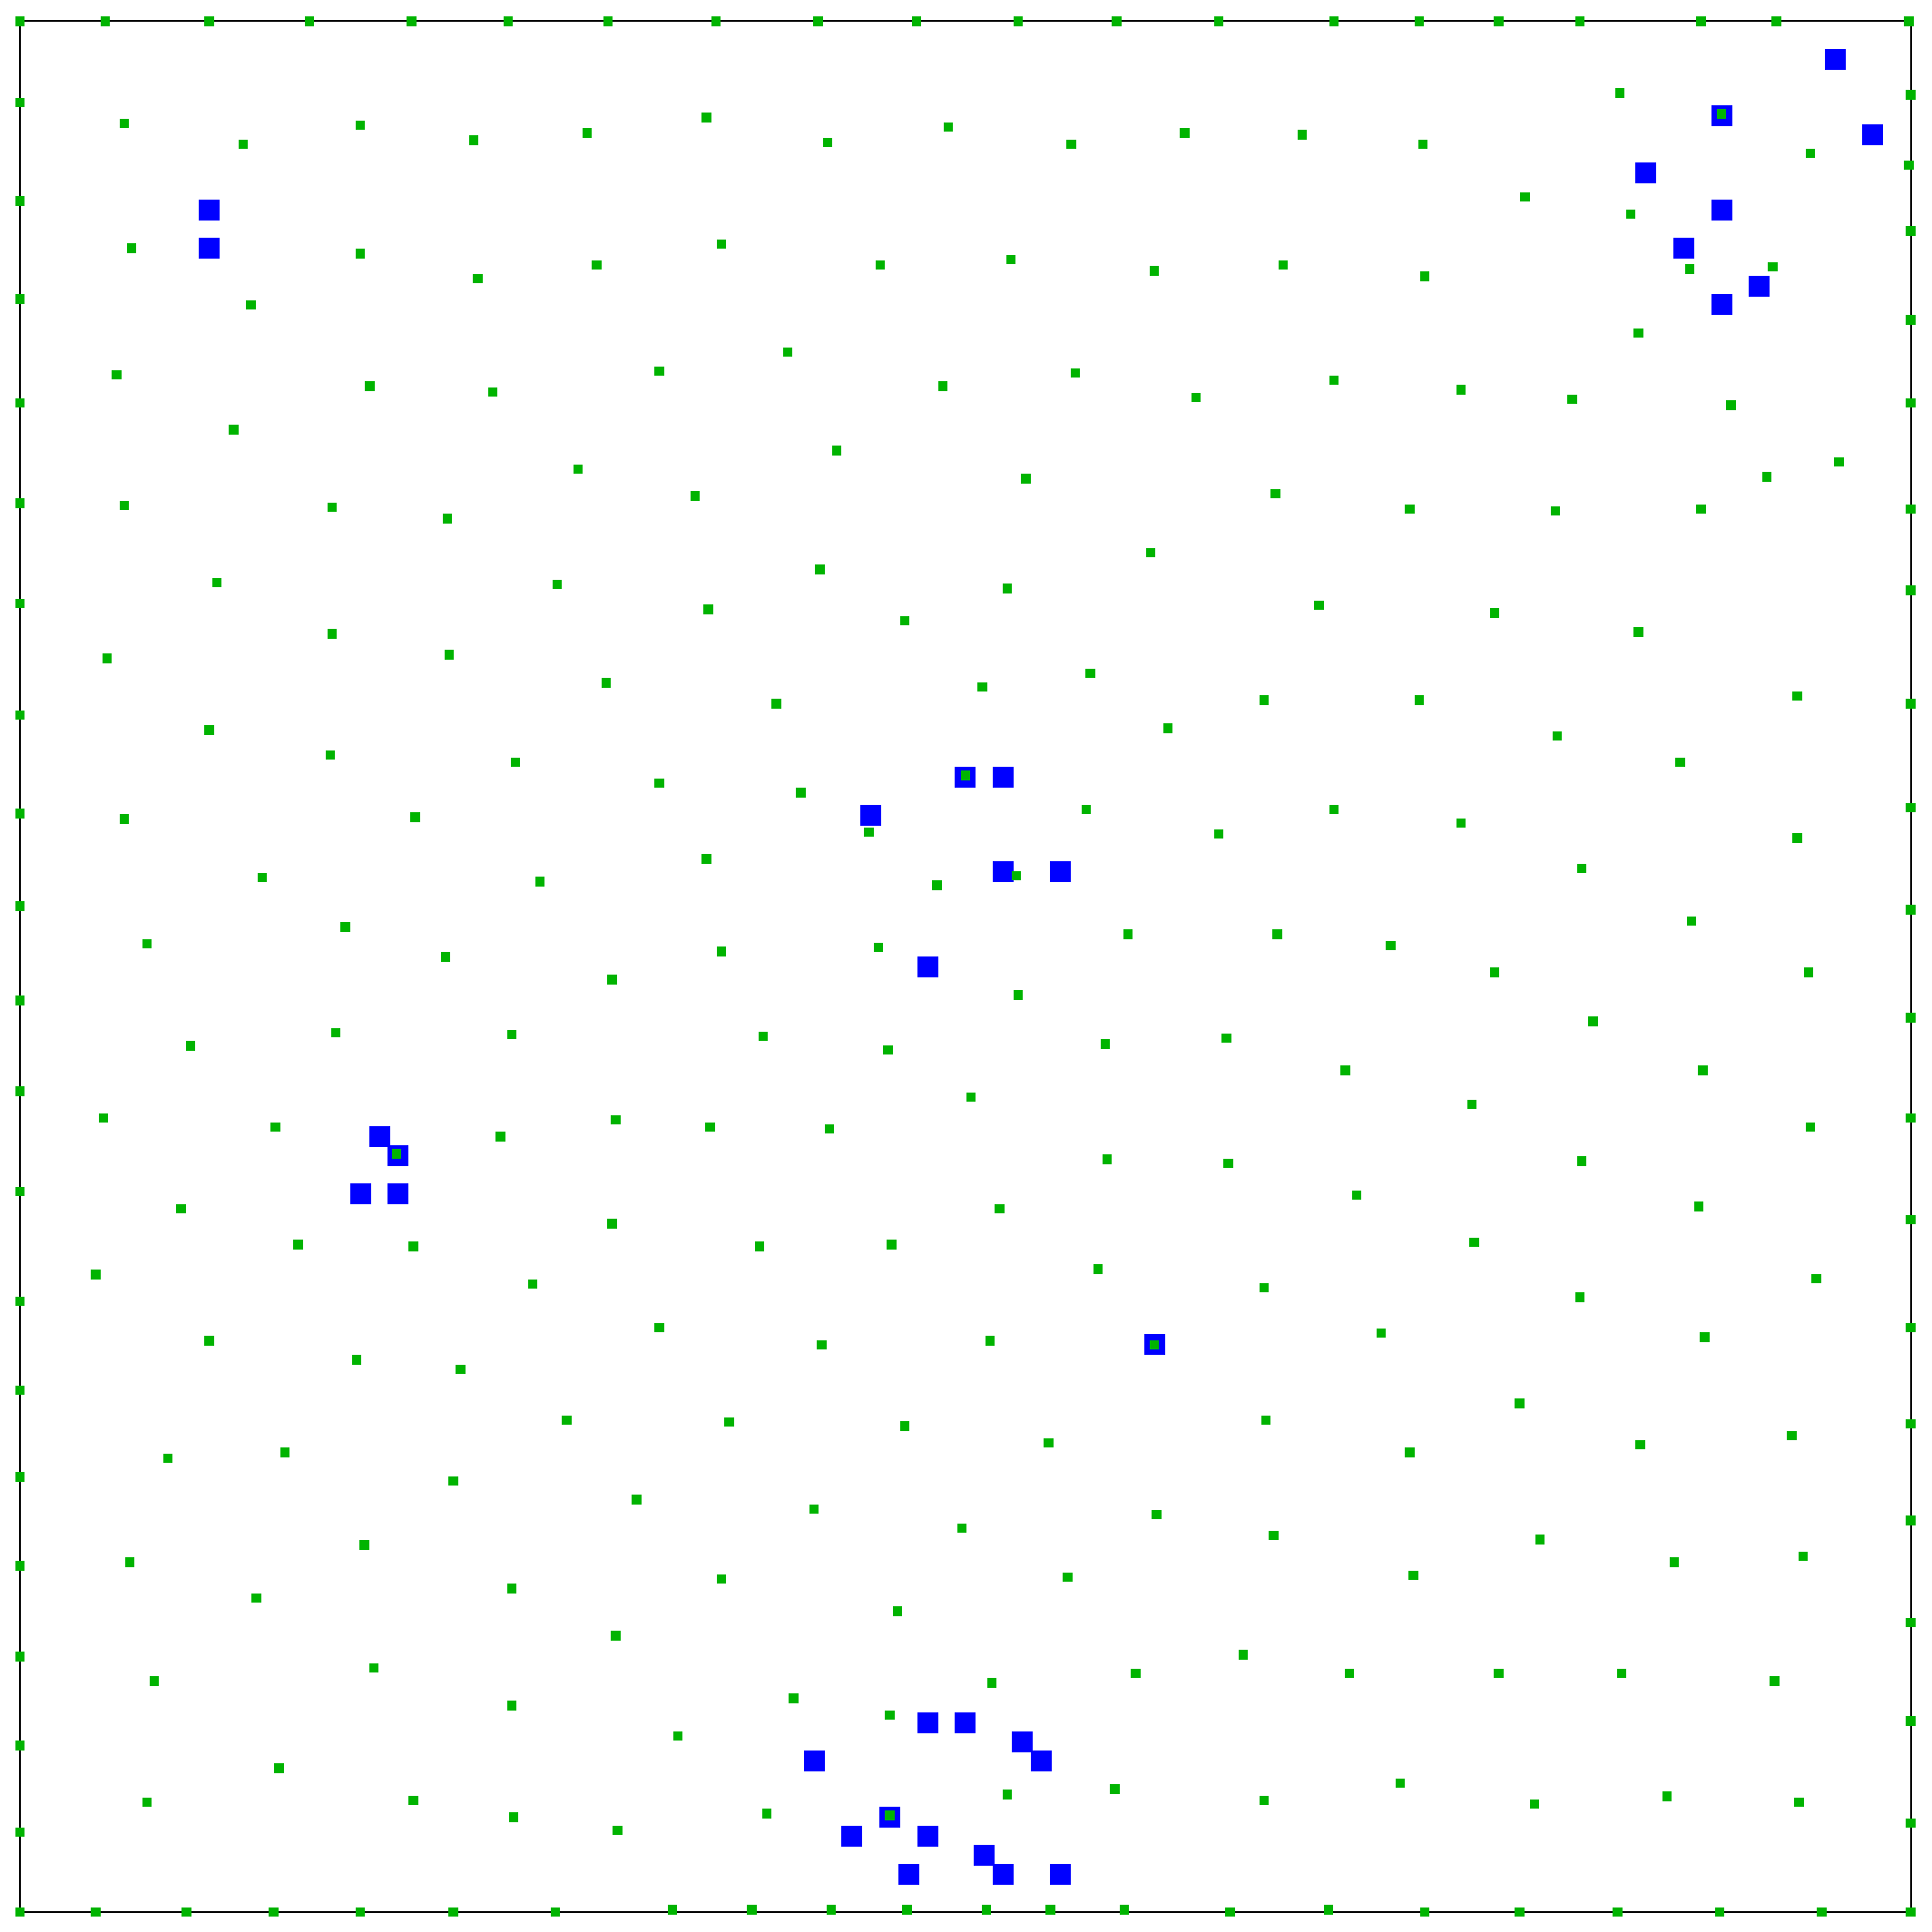
\includegraphics[width=0.5\textwidth]{img/usage/nousage-full.eps}}
  \caption{Test odpudivosti uzl�, jejich napln�nost nen� br�na v uvahu.}
  \label{fig:usage-ag-no}
\end{figure}

\begin{figure}[p]
  \centering
  \subfloat[EmptyRoom]{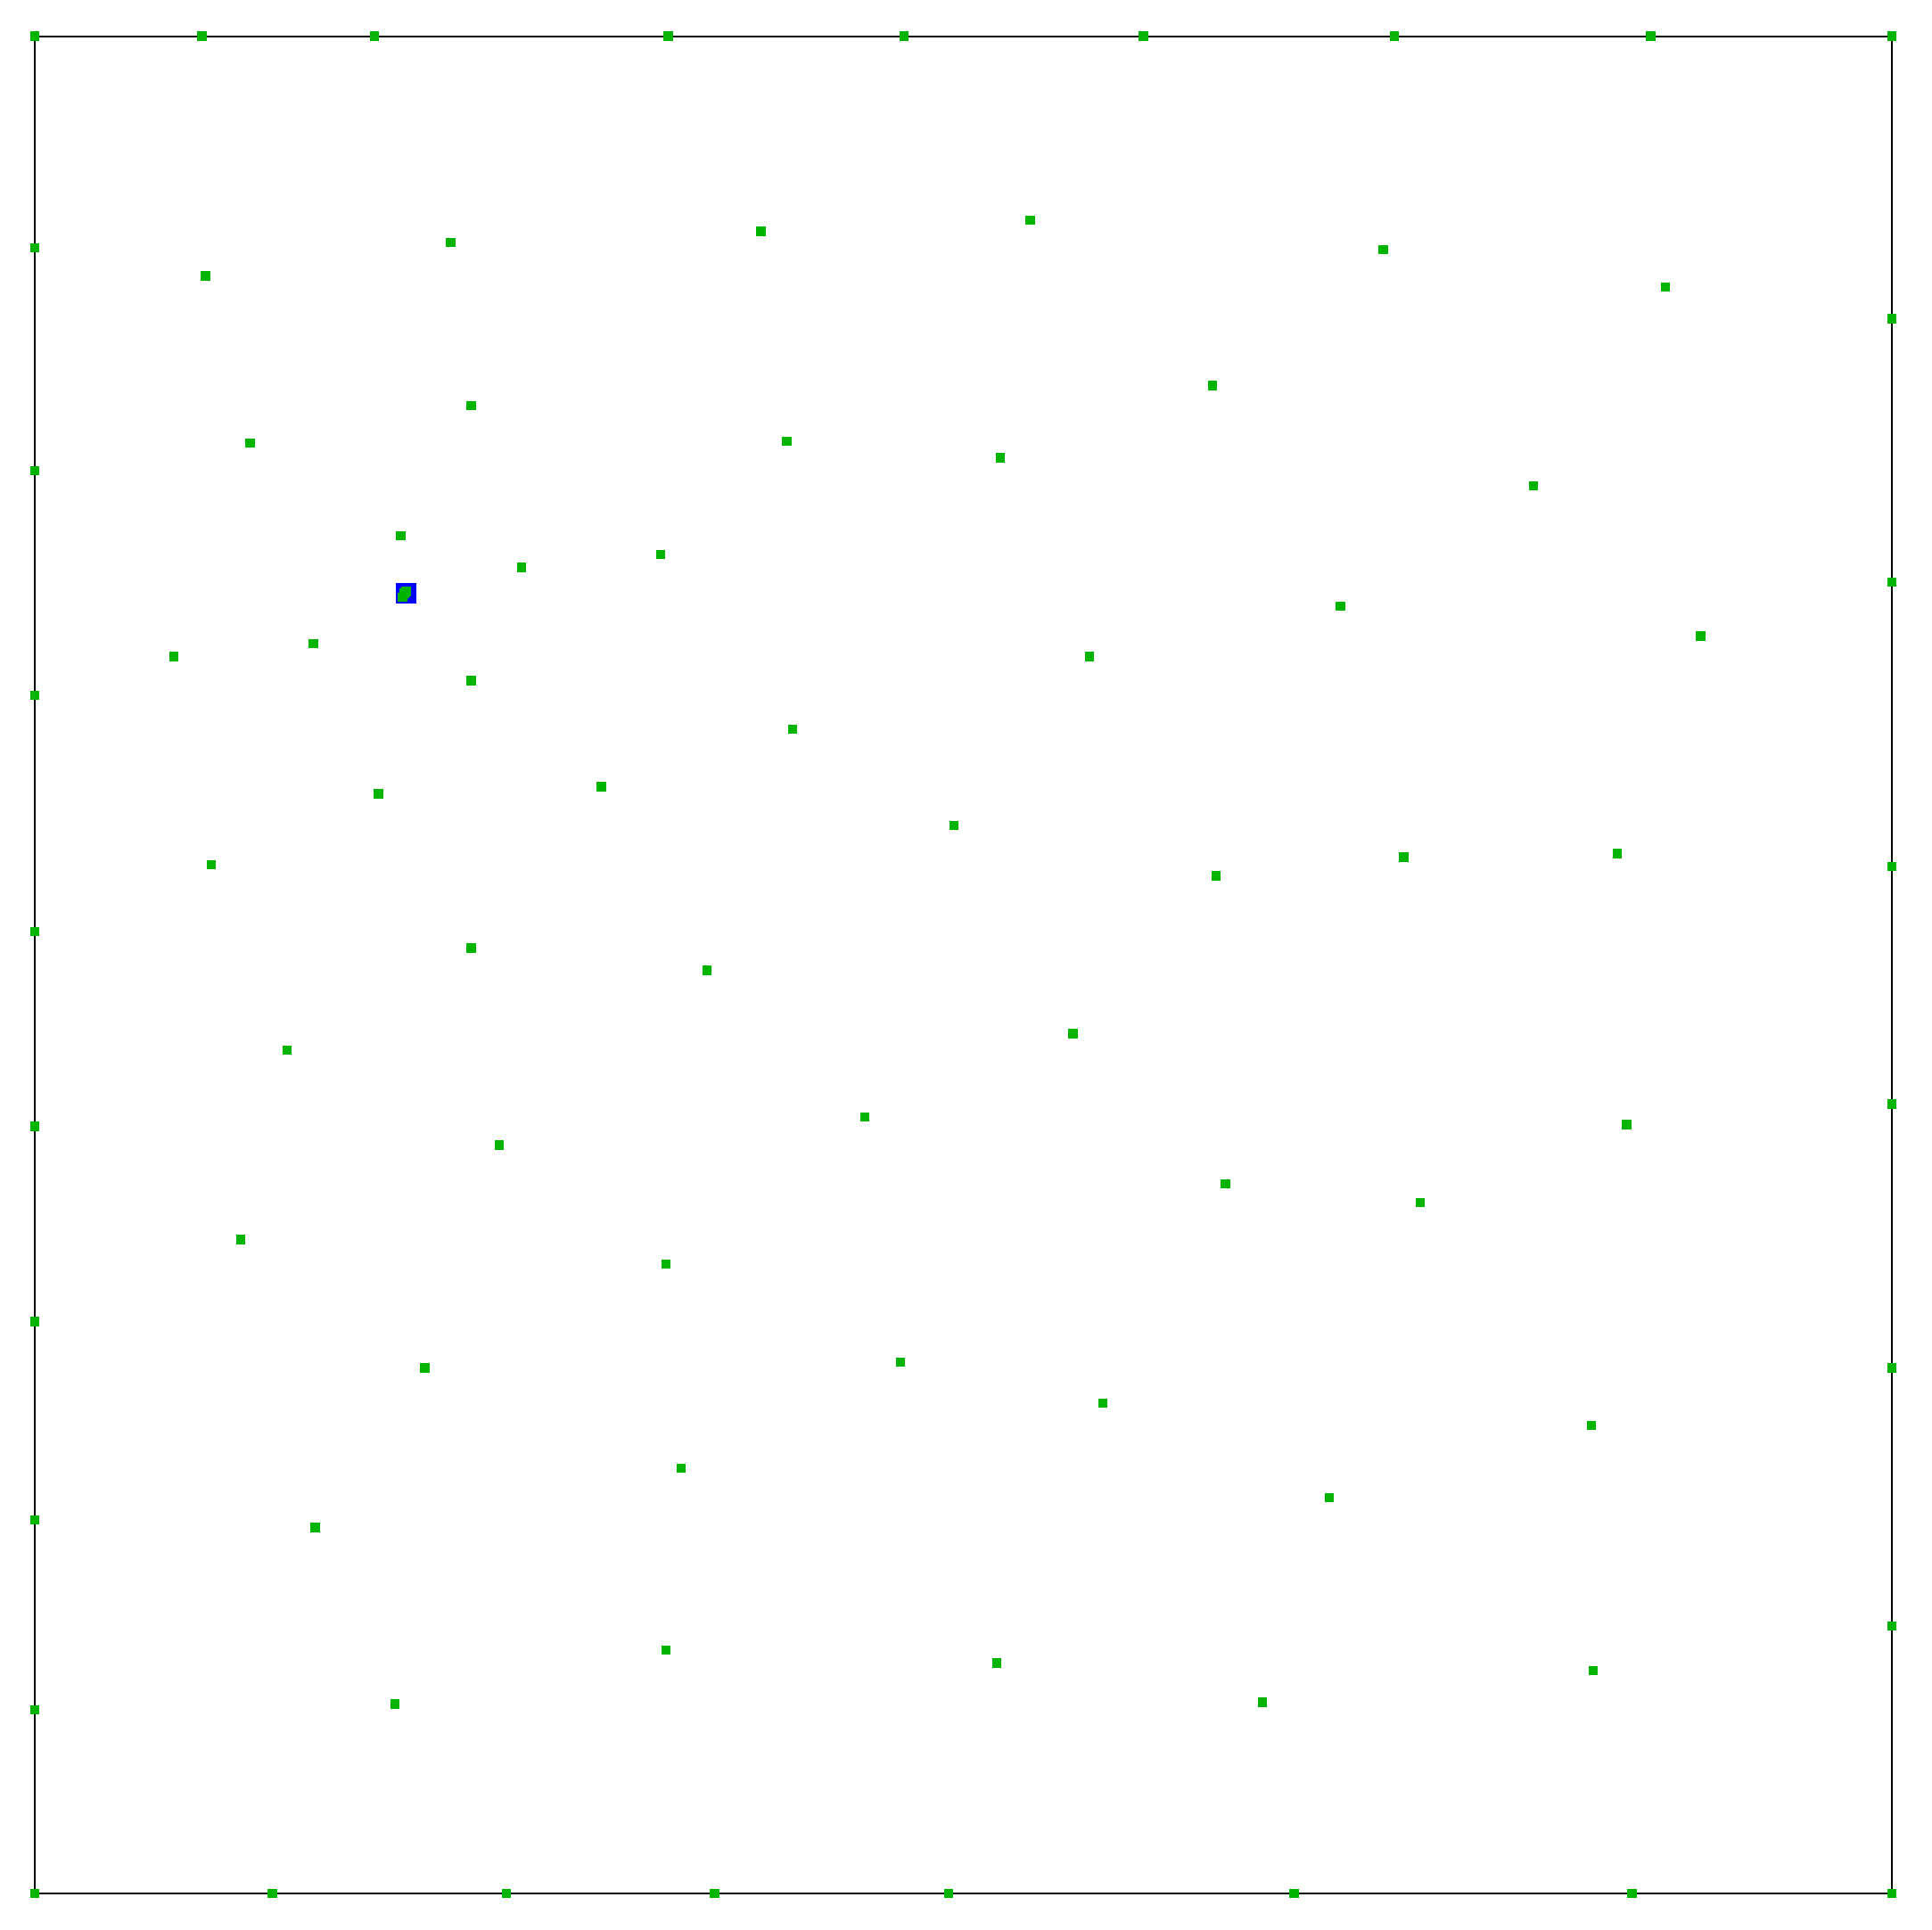
\includegraphics[width=0.5\textwidth]{img/usage/usage1-empty.eps}}
  \subfloat[FullRoom]{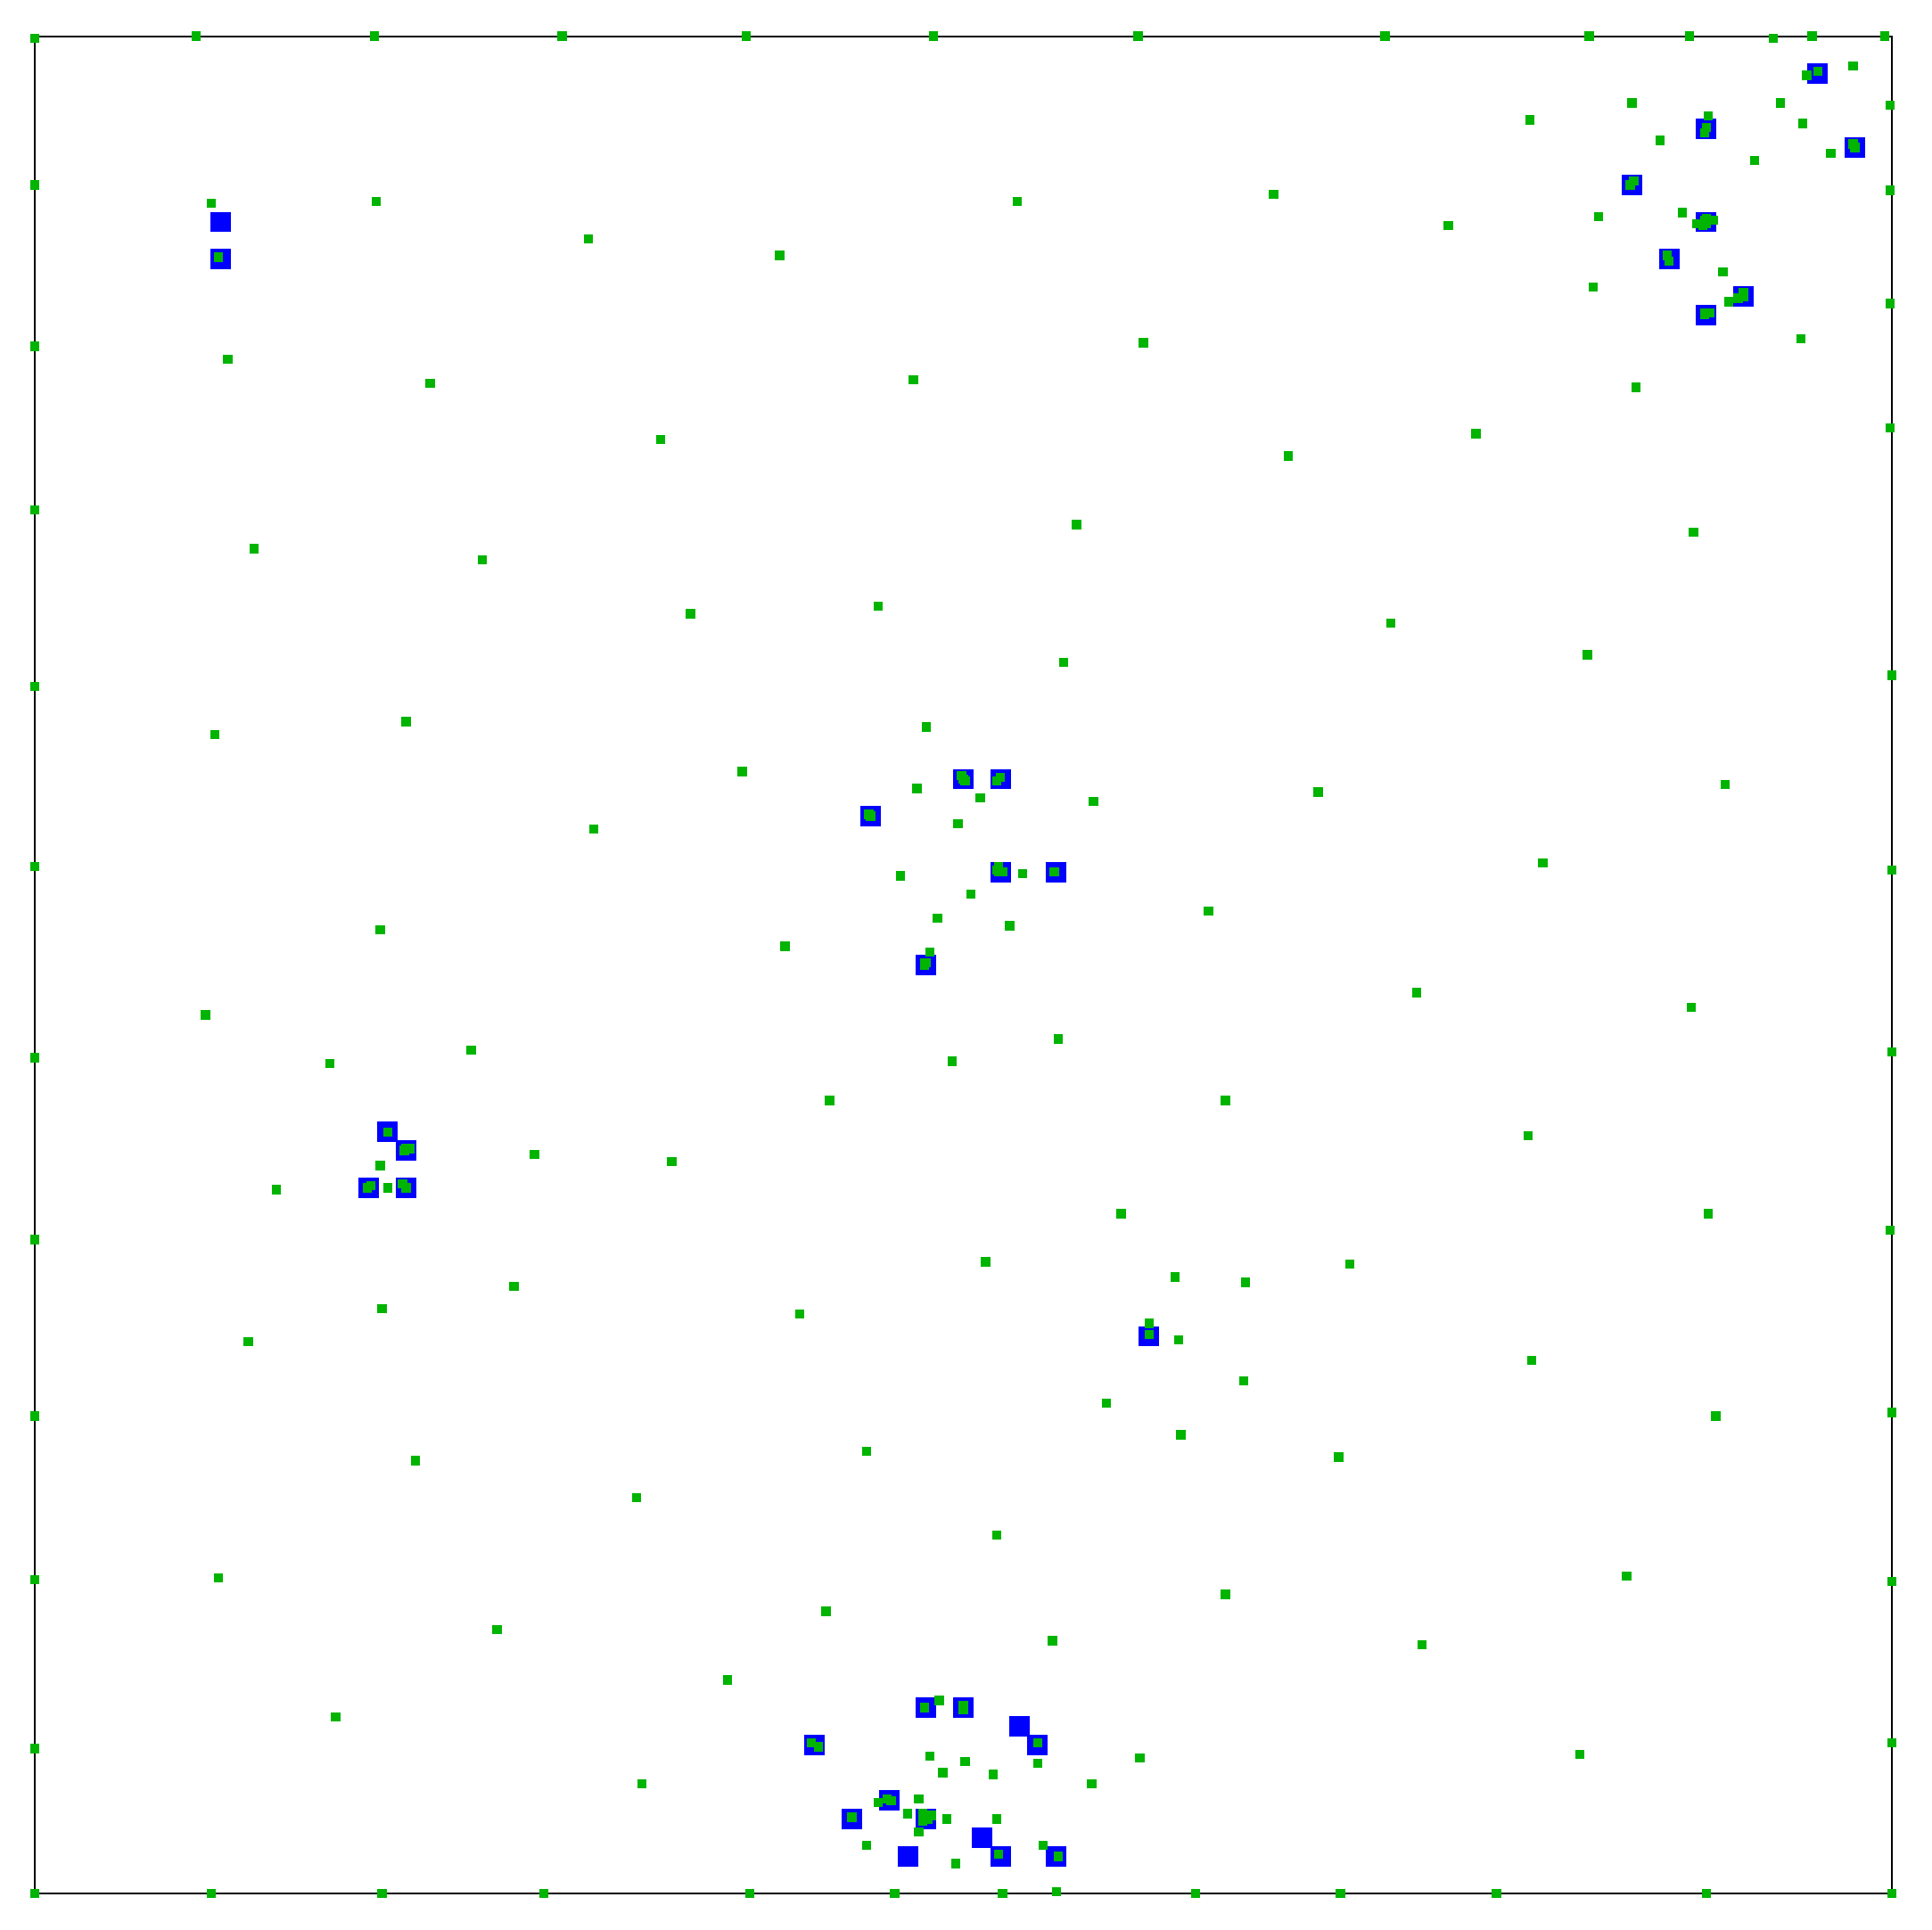
\includegraphics[width=0.5\textwidth]{img/usage/usage1-full.eps}}
  \caption{Test odpudivosti uzl�, vliv napln�nosti $=1$.}
  \label{fig:usage-ag-1}
\end{figure}

\begin{figure}[p]
  \centering
  \subfloat[EmptyRoom]{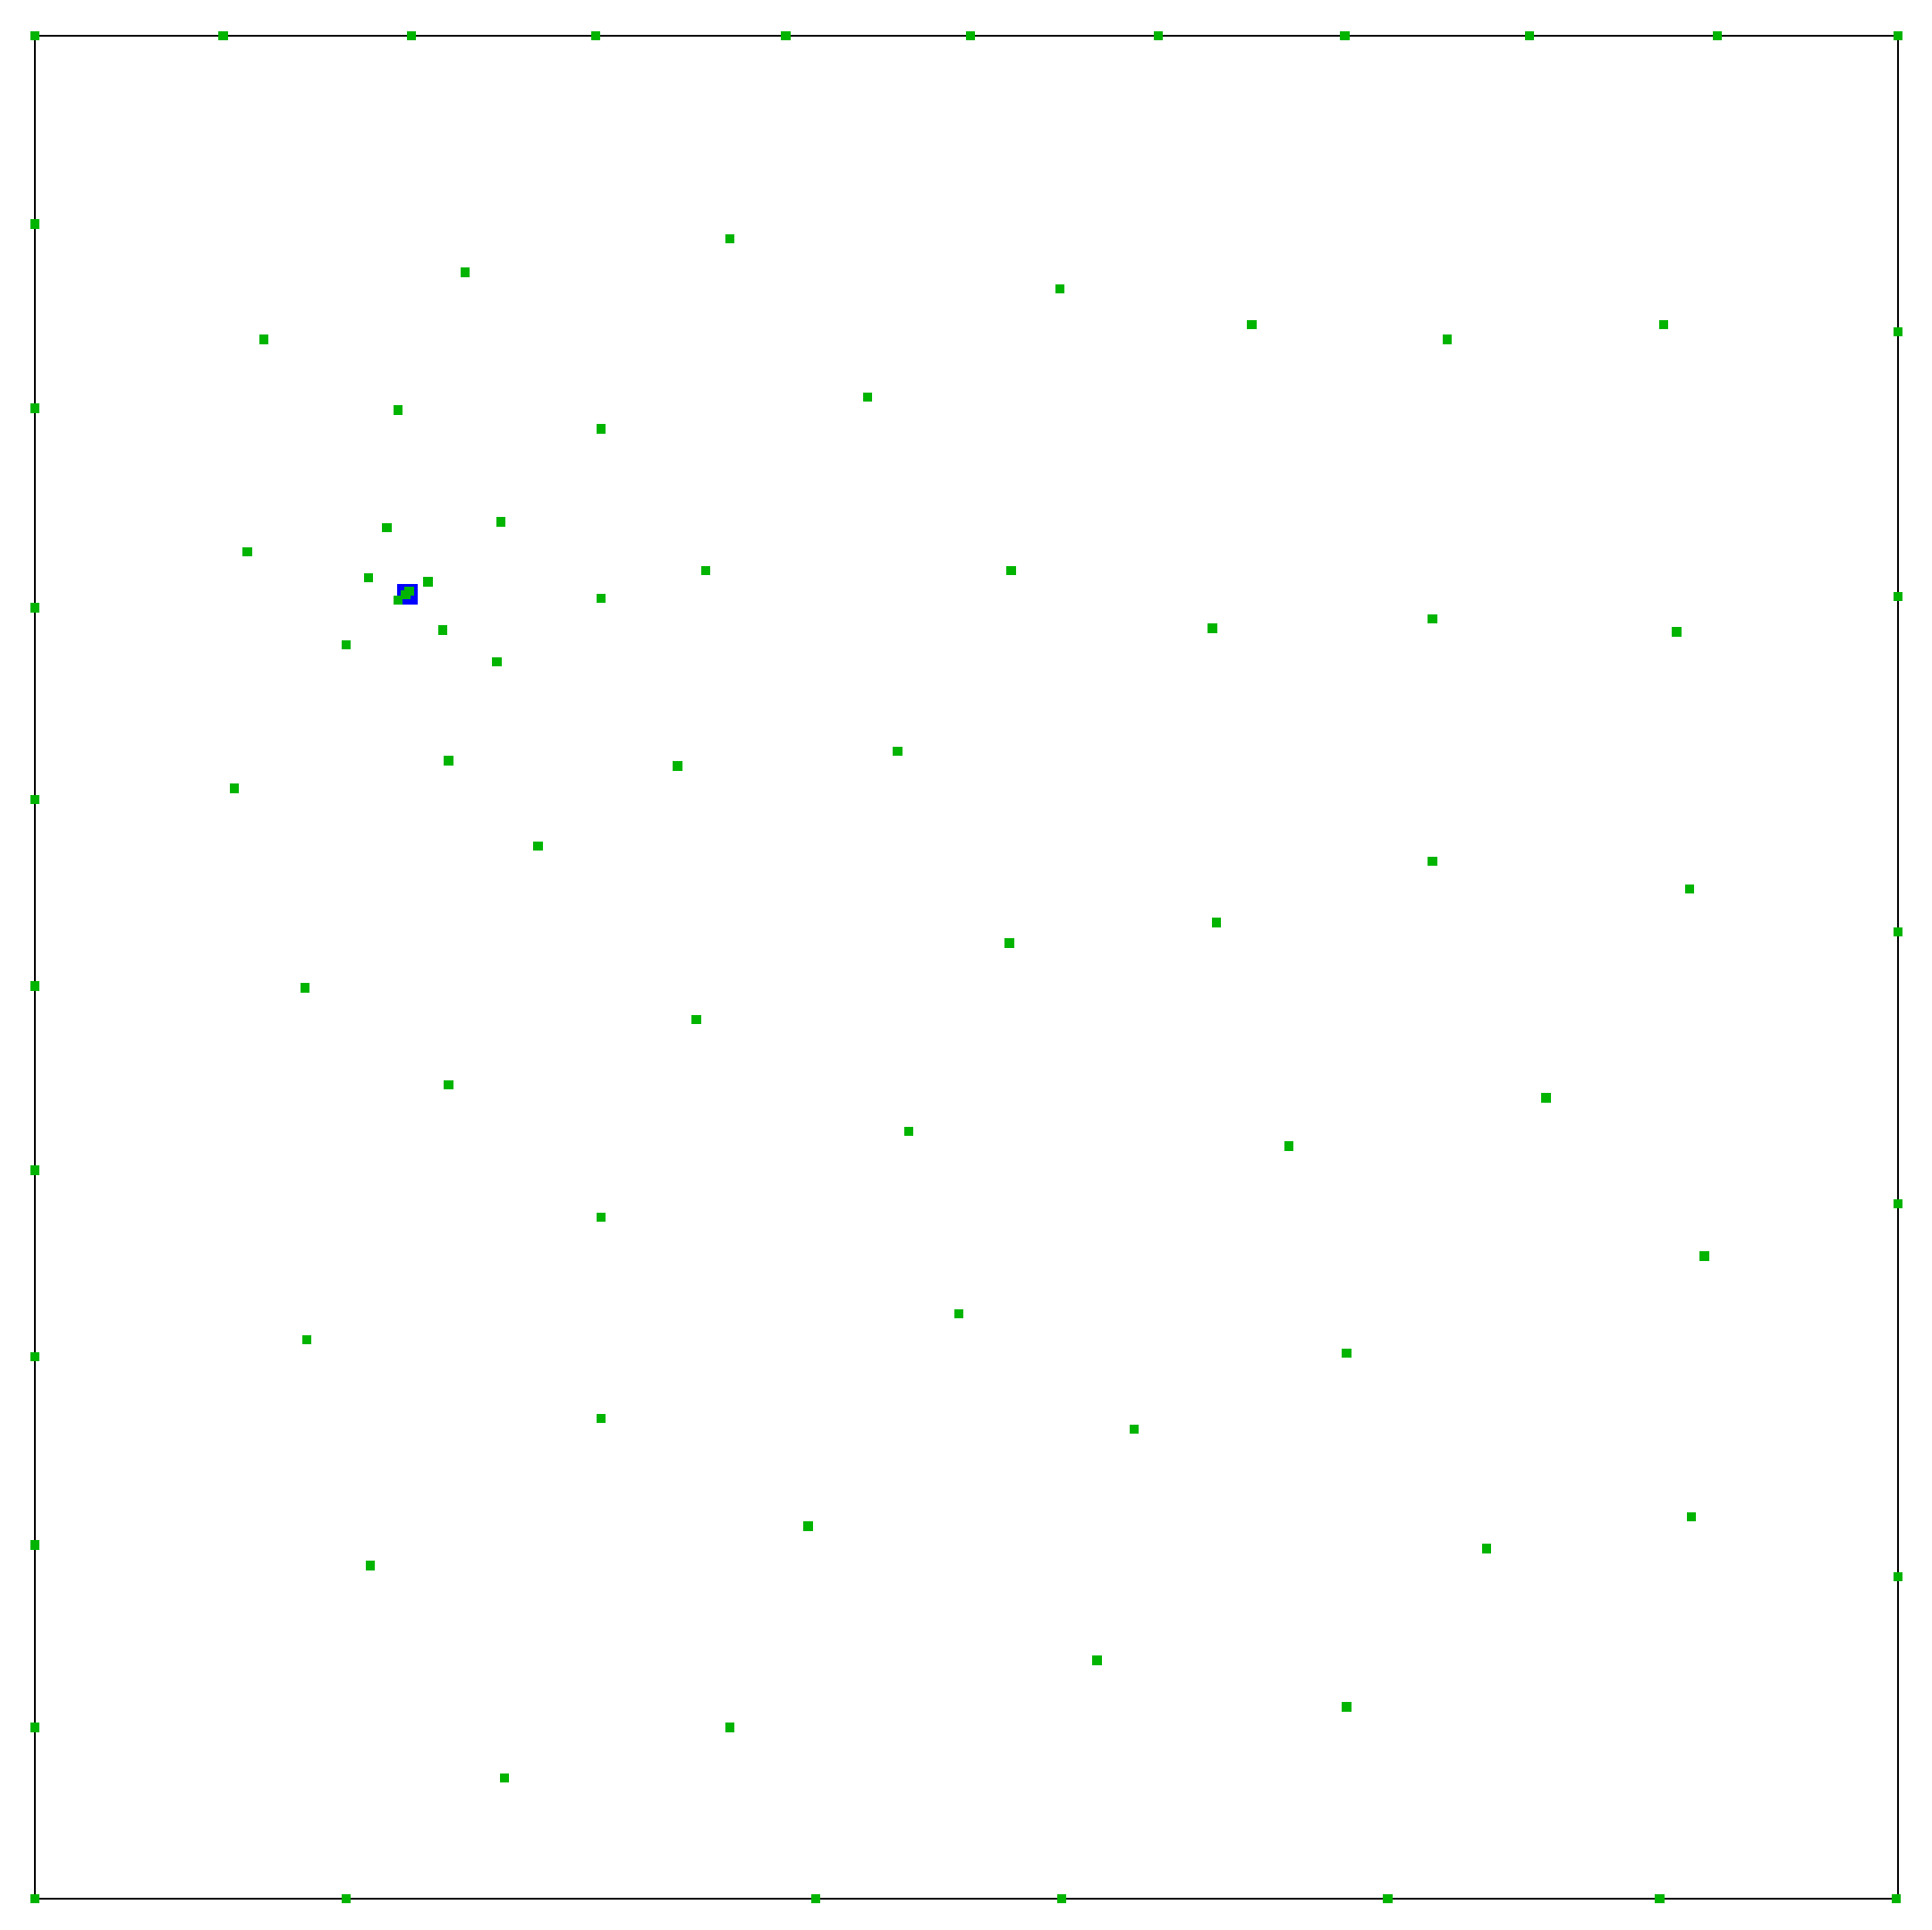
\includegraphics[width=0.5\textwidth]{img/usage/usage0.8-empty.eps}}
  \subfloat[FullRoom]{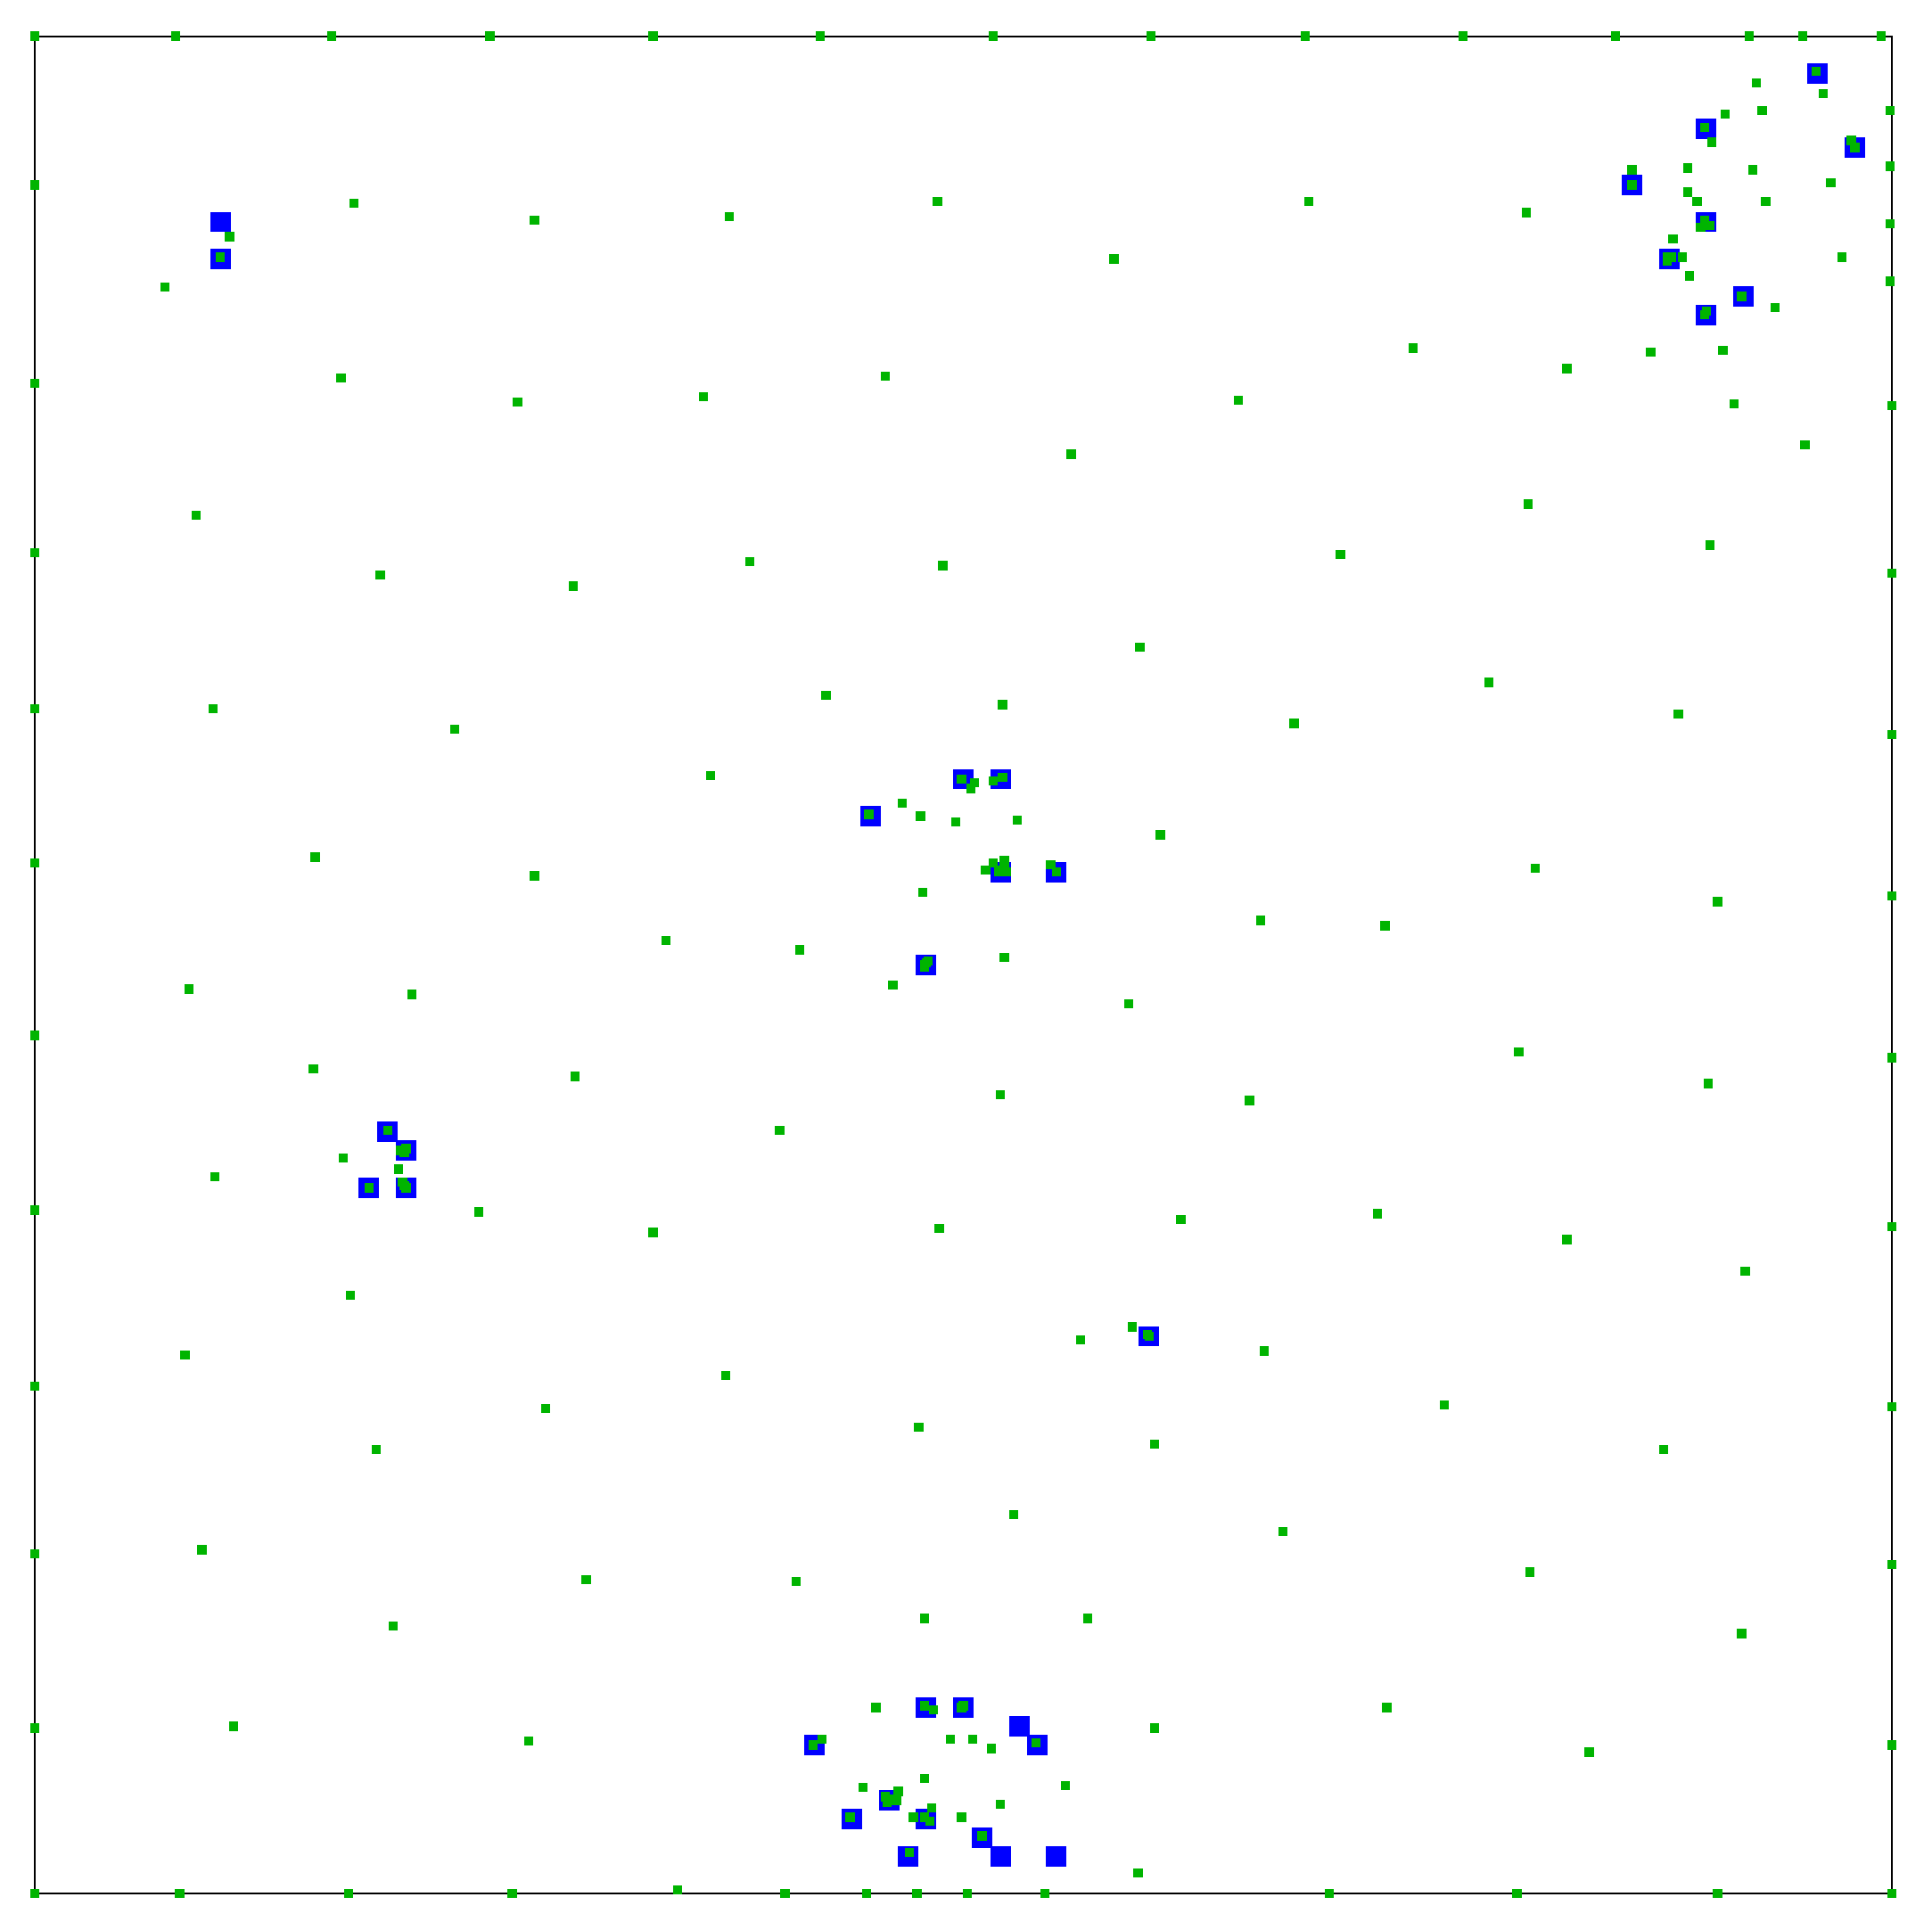
\includegraphics[width=0.5\textwidth]{img/usage/usage0.8-full.eps}}
  \caption{Test odpudivosti uzl�, vliv napln�nosti $=0,8$.}
  \label{fig:usage-ag-0.8}
\end{figure}

\begin{figure}[p]
  \centering
  \subfloat[EmptyRoom]{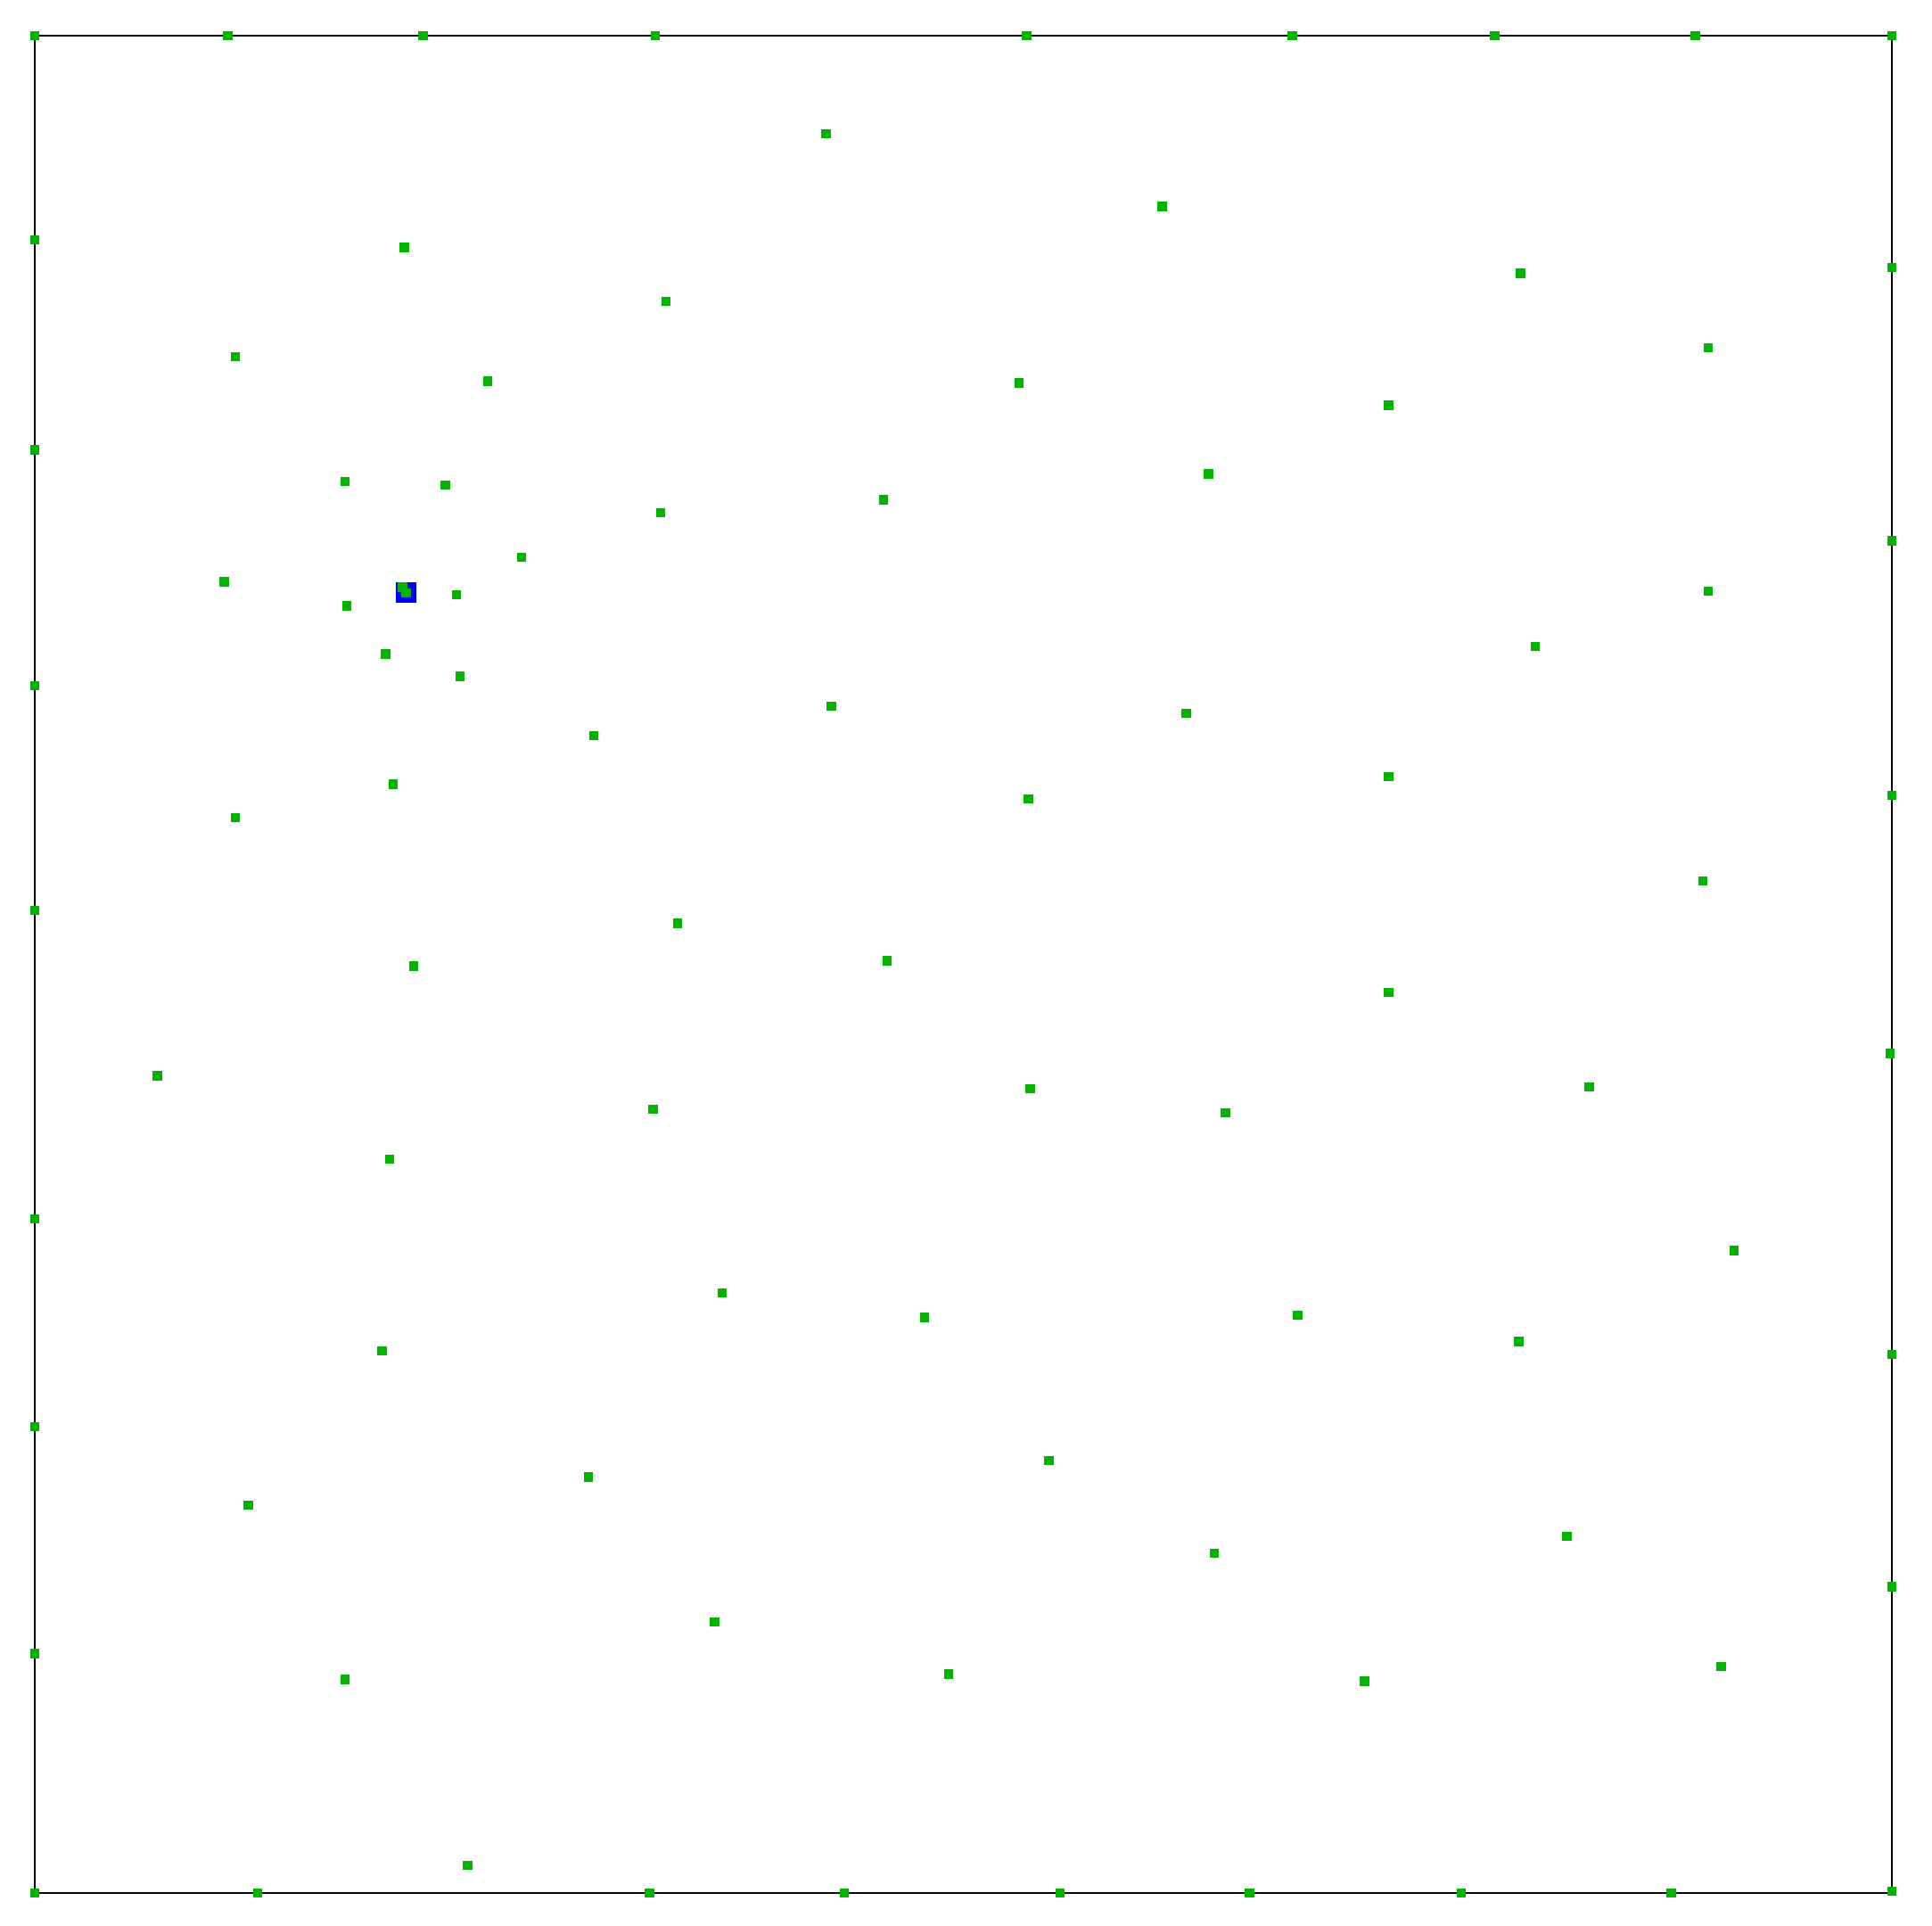
\includegraphics[width=0.5\textwidth]{img/usage/usage0.5-empty.eps}}
  \subfloat[FullRoom]{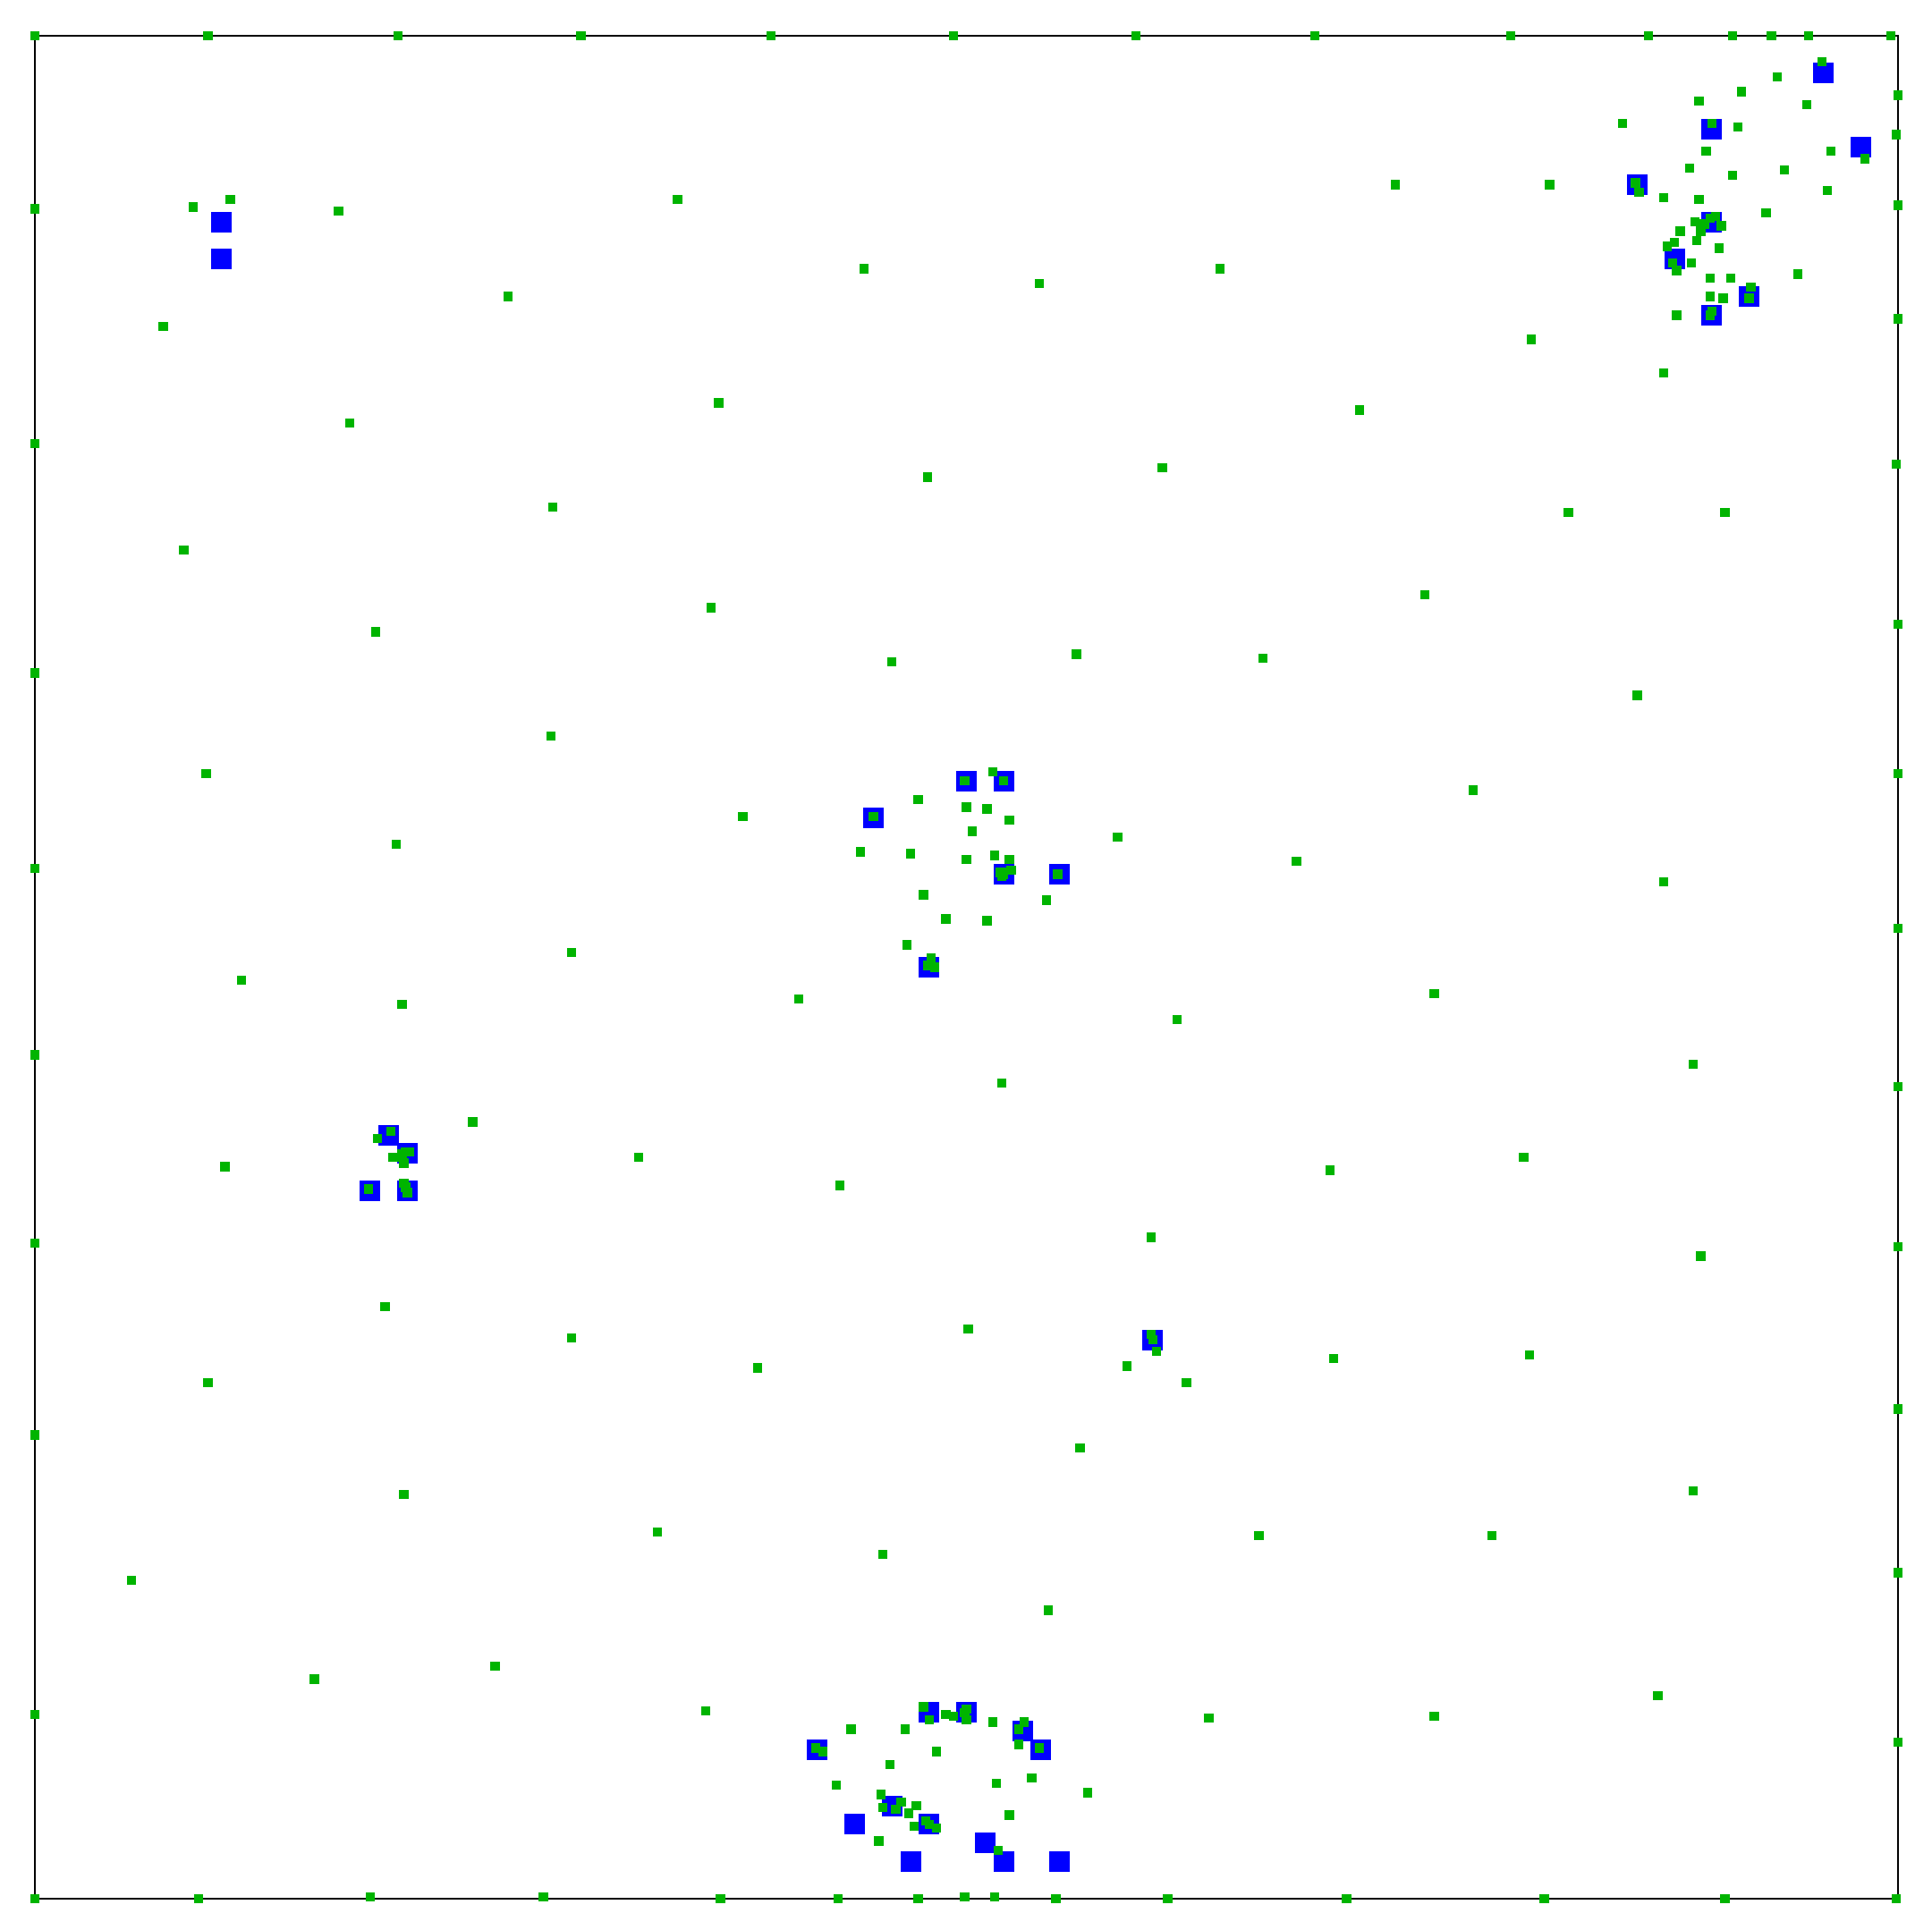
\includegraphics[width=0.5\textwidth]{img/usage/usage0.5-full.eps}}
  \caption{Test odpudivosti uzl�, vliv napln�nosti $=0,5$.}
  \label{fig:usage-ag-0.5}
\end{figure}





Pohyb, vliv na chybu
\\

Ruzna odpudivost
\\
\chapter{Diskuze}
Model prostorov� mapy popsan� v kapitole \ref{chapter-model} resp. \ref{chapter-model-el} spl�uje z�kladn� po�adavky, kter� jsme na n�j kladli.
V pr�b�hu jeho testov�n� a vytv��en� se v�ak objevila cel� �ada mo�n�ch roz���en� a vylep�en�.
N�kter� z nich jsou pops�na v t�to kapitole.
\\

\section{P�ita�livost stop vjemu}
Pokud je v m�stnosti oblast, kde je pobl� sebe v�ce p�edm�t�, prostorov� mapa v n� vytvo�� v�ce uzl�.
Pokud v�ak budou m�t p�edm�ty n�zkou aktraktivitu, nap�. $^1/_{10}$ v�choz� atraktivity, nedojde k vzniku nov�ch uzl�.
Po��te�n� intenzita stop vjemu vytv��en�ch v t�to oblasti bude p��lis mal�, ne� aby pokryla rostouc� cenu uzlu.
P�esto�e v oblasti jich bude hodn�, ��dn� z nich nebude dost intenzivn�.
\\

Pokud �lov�k vid� hromadu mal�ch nezaj�mav�ch v�c�, nezapamatuje si jednotliv� v�ci, zapamatuje si v�ak fakt, �e v dan� oblasti byla \uv{velk� hromada n��eho}.
�e�en�m by bylo p�idat do modelu p�ita�livost stop vjemu. Lze ji ch�pat jako shlukov�n� vjem�, kter� jsou bl�zko u sebe.
S�la p�ita�livosti by m�la b�t nep��mo �m�rn� intenzit� stopy vjemu, budou se tak shlukovat pouze vjemy s malou intenzitou.
Tak� ochota stopy m�nit svou polohu, tedy velikost zm�ny polohy, by m�la b�t nep��mo �m�rn� jej� intenzit�.
V�sledkem bude, �e slab�� vjemy budou p�itahov�ny k siln�j��m.
\\

% ?? ToDo ukazat/overit na prikladu na prikladu, ze to tak je.

\section{Adaptivn� odpudivost}
V p�edstaven�m modelu je vz�jemn� odpudivost uzl� z�visl� pouze na jejich vzd�lenosti a napln�nosti.
Je d�le ovlivn�na parametry modelu, kter� jsou v�ak v pr�b�hu cel� simulace konstantn�.
\\

Jedna z mo�nost�, jak zlep�it rozlo�en� uzl� v prostoru, je m�nit parametry ovliv�uj�c� odpudivost,
v pr�b�hu simulace, p�edev��m \param{s�lu odpudivosti} a \param{dosah odpudivosti}.
Parametry by se mohly m�nit podle aktu�ln� hustoty uzl�, kter� se odr�� v mno�stv� odpudivosti.
Dal��m �e�en�m by bylo p�idat je do v�po�tu odpudivosti,
t�m by parametry p�estaly b�t stejn� pro v�echny uzly a odpudivost uzl� by se tak p�izp�sobovala lok�ln� situaci.
\\


\section{Sjednocen� stopy vjemu a uzlu}
V p�edstaven�m modelu jsou dva podobn� objekty: stopa vjemu a uzel prostorov� mapy.
Na stopu vjemu lze nahl�et jako na do�asn� uzel mapy, kter� m� danou svou �ivotnost.
Sou�asn� lze nahl�et na uzel mapy jako na trvalej�� stopu vjemu.
Stopa vjemu a uzel jsou tedy jen dva r�zn� stupn� t�ho� typu objektu, stopa vjemu je uzel nult�ho stupn�.
\\

Model lze roz���it o dal�� stupn�. Uzly by vytv��ely dal�� uzly, kter� by m�ly je�t� trvalej�� charakter.
Stupe� uzlu by ur�oval jeho trvalost, ochotu se pohybovat a m�ru, s jakou vytv��� dal�� uzly vy���ho stupn�.
�pln�m zobecn�n�m modelu by byla zm�na stupn� uzlu z diskr�tn� veli�iny na spojitou. Mapa by tak obsahovala mnoho uzl� r�zn�ho stupn�.
\\



\section{Zapom�n�n�}
Model obsahuje n�kolik mechanism� pro zapom�n�n�:

\begin{CompactItemize}
\item sni�ov�n� intenzit pam�ov�ch stop a vazeb mezi stopou a uzlem
\item sl�bnut� a zmizen� stop vjemu
\item kles�n� napln�nosti uzlu
\item kles�n� mno�stv� odpudivosti uzlu
\item zapom�n�n� uzl�
\item kles�n� intenzity m�sta
\end{CompactItemize}

Zapom�n�n� uzl� je mo�n� roz���it n�kolika zp�soby.
Cenu vytvo�en� a zapomenut� uzlu je mo�n� skl�dat z v�ce exponenciel, aby bylo dosa�eno pozvoln�j��ho pr�b�hu funkce a dal��ho zpomalen� zapom�n�n� uzl�.
D�le je mo�n� p�i zapom�n�n� uzl� br�t v potaz jejich napln�nost. 
Zapomenut� uzl� s r�znou napln�nost� by nem�lo m�t stejnou cenu zapomenut� uzlu $cost_forget$, uzel s vy��� napln�nost� je pro mapu d�le�it�j��.
To se m��e prom�tnout do sni�ov�n� energie na zapom�n�n�, je� bude sni�ov�na v z�vislosti na napln�nosti uzlu, kter� byl zapomenut.
Tak� samotn� v�b�r uzlu, kter� bude zapomenut, m��e b�t ovlivn�n jejich napln�nost�.
\\

Sl�bnut� a kles�n� r�zn�ch vlastnost� uzl�, vazeb a m�st je v p�edstaven�m modelu line�rn�, nez�vis� na aktu�ln� hodnot� vlastnosti.
Model by bylo vhodn� roz���it, aby rychlost kles�n� z�visela na jej� aktu�ln� hodnot�.
Pokud je hodnota vysok�, kles� rychleji, pokud se hodnota bl�� k nule, kles� ��m d�l pomaleji.
\\

Model �e�� zapom�n�n� pouze za relativn� kr�tkou dobu.
P�eneseme-li m���tko �asu modelu, tj. kroky simulace, do re�ln�ho sv�ta, je vid�t, �e model vyhovuje pro dobu trvaj�c� ��dov� jednotky a� des�tky t�dn�.
Pokud by model m�l uspokojiv� �e�it zapom�n�n� v ��du let, bylo vhodn� roz���it intezitu vjemu do komplexn�j�� veli�iny,
nap�. p�idat mechanismy pracuj�c� s emocemi.
\\



\section{Roz���en� uzlu a m�sta}
Do uzlu je v modelu ukl�d�na pouze informace o poloze p�edm�t�.
Uzly lze v�ak vyu��t i k uchov�n� dal��ch informac�, nap�. kter� �innosti pobl� nich agent prov�d�l.
Vznikla by asociativn� s� vazeb mezi �innostmi a uzly. Jin�m �e�en�m by bylo vytv��et v�ce map, pro ka�d� typ uchov�van� informace jednu.
\\

Ukl�dan� informace pak mohou b�t propagov�ny z uzl� do m�st a z nich do nad�azen�ch m�st.
Agent by pak byl schopen ur�it nej�ast�j�� �innosti prov�d�n� v ur�it� m�st� a vytvo�it si tak p�edstavu o jeho funk�nosti,
nap�: m�sto, kde se nej�ast�ji j� a p�ipravuje j�dlo, ozna�� jako m�sto k tomu ur�en�.
Pokud bychom mu dodali dostatek informac�, bude schopen jej ozna�it slovem \emph{j�delna} �i \emph{kuchyn�}.
K tomu ��elu by bylo t�eba vytvo�it hierachii afordanc� �i je n�jak jinak kategorizovat.
\\

Model byl vytvo�en v prost�ed� sv�ta jen s jedn�m agentem.
Pokud by sv�t obsahoval v�ce agent�, objevily by se dal�� informace, kter� by bylo mo�n� ukl�dat,
nap�. kde se agent setkal s jin�m konkr�tn�m agentem �i co vid�l d�lat ostatn� agenty.
Pokud by spolu agenti komunikovali, mohli by si p�ed�vat informace o poloze p�edm�t�.
Takov� informace je pak z hlediska modelu prostorov� mapy jen dal�� typ vjemu, jeho� intenzita by z�visela nap�. na d�v�ryhodnosti agenta.
Cel� proces p�ed�n� informace o poloze p�edm�tu agentem $a_1$ agentovi $a_2$ si pak lze p�edstavit takto:
\begin{CompactItemize}
\item agent $a_1$ si vybav� pam�ovou stopu a vytvo�� si pam�ov�ho fantoma
\item pam�ov� fantom je p�ed�na agentovi $a_2$
\item agent $a_2$ vytvo�� na z�klad� pam�ov�ho fantoma vjem, jeho� intenzita bude odvozena z intenzity pam�ov� stopy agenta $a_1$ a dal��ch faktor�
\item prostorov� mapa agenta $a_2$ zpracuje vjem
\end{CompactItemize}


Ulo�enou pozici objektu\footnote{pam�ovou stopy v prostorov� map� agenta $a_2$}
by bylo vhodn� obohatit o informaci, �e tuto polohu se agent dozv�d�l od jin�ho agenta a od kter�ho.
Zde je mo�n� model d�le obohacovat, agent m��e nap�. po �ase zapomenout, kdo mu poloze p�edm�tu sd�lil.
\\




\section{Roz���en� modelu pro slo�it�j�� sv�ty} \label{chapter-complex-space}
Model je navr�en pro velmi jednoduch� sv�t obsahuj�c� pouze jednu 2D m�stnost.
Tato kapitola p�edstavuje roz���en� modelu pro sv�t obsahuj�c� v�ce m�stnost�, kter� jsou 3D.
\\

Roz���en� modelu do 3D je p��mo�ar�. V�echny algoritmy a vzorce pracuj� nez�visle na dimenzi sv�ta.
Poloha objekt� prostorov� mapy bude ur�ena t�emi sou�adnicemi $<x,y,z>$. Vzd�lenost mezi objekty bude euklidovsk�:
\begin{equation} 
dist_{3D}(a,b) = \sqrt{  (a_x-b_x)^2 + (a_y-b_y)^2 + (a_z-b_z)^2}.
\label{formula:vzdalenost-3D}
\end{equation}
M�stnost m��e b�t obecn� mnoho�heln�k. Model pot�ebuje od vn�j��ho sv�ta pouze n�sleduj�c� rozhran�: 
\begin{CompactItemize}
\item ur�it obsah mnohost�nu
\item testovat n�le�en� bodu do mnohost�nu
\item ur�it pr�se��k �se�ky a st�ny
\item ur�it viditelnost p�edm�tu\footnote{Zorn� pole, popsan� v kapitole \ref{chapter-agent} jako kruhov� v�se�e, budou ku�ely.}
\end{CompactItemize}

Implementace t�chto funkc� bude kl�st v�razn� v�t�� n�roky na v�po�etn� v�kon, ne� model v 2D sv�t�.
Pro tyto ��ely by bylo vhodn� vyu��t hotov� �e�en�, nap�. n�jak� voln� dostupn� hern� �i fyzik�ln� engine.
\\


Sv�t kolem n�s nen� omezen na jednu uzav�enou m�stnost, skl�d� se z mnoha prostor�, kter� se d�l� na men�� a men��.
Sv�t kolem n�s m��eme ch�pat jako hiearchii takov�ch prostor�, i kdy� hranice mezi nimi nejsou v�dy jasn� ur�en�.
Nap�. d�m se d�l� na podla��, ta d�le na byty, kter� jsou slo�eny z n�kolika m�stnost�.
Model je mo�n� roz���it tak, aby dok�zal pracovat ve sv�t� ur�en�m jako hiearchie prostor�.
\\

\begin{definition}[Hiearchick� sv�t]
Sv�t se skl�d� z prostor�. Ka�d� prostor je obecn� mnoho�heln�k, rozd�len� na dal�� podprostory. T�m je vytvo�ena hiearchie prostor�.
Ko�en stromu t�to hiearchie je samotn� sv�t, listy stromu jsou prostory, kter� ji� nem� smysl d�le d�lit, nap�. mal� uzav�en� m�stnost, ledni�ka �i police.
Podprostory v prostoru jsou ch�p�ny jako p�edm�ty, nap�. ledni�ka je prostor obsahuj�c� p�edm�ty, ale z hlediska m�stnosti je pouze p�edm�tem.
\end{definition}

��st prostorov� mapy \emph{pam� na p�edm�ty} pracuje nez�visle na velikosti sv�ta.
\emph{Vrstva uzl�} je na n�m z�visl�, proto si mapa vytvo�� novou pro ka�d� prostor.
V d��ve uveden�m p��kladu domu by ka�d� m�stnost, byt i podla�� m�ly vlastn� \emph{vrstvu uzl�}.
Hiearchii sv�ta mus� model dostat k dispozici. \footnote{
 Model by si tuto hiearchii mohl konstruovat s�m obdobn�m zp�sobem, jak�m si vytv��� m�sta v kapitole \ref{chapter-place-detect}.
 Pak by m�l pouze jednu velmi rozs�hlou vrstvu uzl�.
 To by nebylo vhodn� z hlediska n�roku na v�po�etn� v�kon. Nav�c lid� tuto hiearchii vn�maj� okam�it�, nemusej� se ji zdlouhav� u�it.
}\\

To nav�c umo��uje parametrizovat vrstv� uzl� na m�ru konkr�tn� m�stnosti, dokonce pou��t jin� implementace a ur�it� modifikace modelu.
Nap�. mal� m�stnost pln� p�edm�t� (sklad) a velk� t�m�� pr�zdn� m�stnost (hala) mohou m�t zcela jin� nastaven� parametr�, jako je hustota mapy �i cena uzlu.
\\



\section{Dal�� mo�n� pou�it� modelu}
Model je navr�en jako ��st episodick� pam�ti virtu�ln�ho agenta. Nen� v�ak z�visl� na jeho architektu�e.
M� ur�it� po�adavky na geometrii virtu�ln� sv�ta, pro kter� vytv��� prostorovou mapu:

\begin{CompactItemize}
\item sv�t je 2D polygon, kter� se vejde do �tverce p�ibli�n� 100$\times$100
\item p�edm�ty nemaj� velikost, jsou reprezentov�ny sv�m st�edem
\end{CompactItemize}

Tyto po�adavky v�ak nejsou pro mnoho �loh z�sadn�m zp�sobem omezuj�c�.
Model je mo�n� pou��t i pro jin� ��ely.
Stru�n� �e�eno, model um� ukl�dat informaci o rozlo�en� p�edm�t� v omezen�m prostoru na z�klad� postupn�ch informac� o jejich poloze.
D�le um� ur�it \emph{m�sta}, tj. oblasti, kde je v�ce p�edm�t�.
\\

Model by bylo mo�n� pou��t nap�. pro vytvo�en� po��ta�ov�ho protivn�ka do hry pexeso.
V ka�d�m kole hry agent vid� dvojici karet - dva vjemy p�edm�t�.
D�ky tomu, �e vjemy maj� intenzitu, m��e model br�t v potaz i fakt, �e agent se na karty d�v� z ur�it�ho uzlu a vzd�lenosti.
Atraktivita p�edm�tu m��e b�t pou�ita pro simulaci rozeznatelnost� obr�zku na kart�.
Jinou atraktivitu bude m�t karta s obr�zkem �erven�ho vyk�i�n�ku a jinou karta s ilustrac� v nev�razn�ch pastelov�ch barv�ch.
Kdy� si bude agent vybavovat polohu karty v p�ru, model ur�� jej� polohu s nep�esnost� odpov�daj�c� po�tu oto�en� hledan� karty.
\\

Dal�� �lohou, kde by bylo mo�n� model pou��t, je u�en� se rozlo�en� kl�ves na kl�vesnici virtu�ln�m agentem a simulace jeho p�eklep�.
Psan�m p�smen, tedy pou��v�n�m kl�ves, by se model rozlo�en� u�il a v pr�b�hu �asu by frekvence p�eklep� klesala.
\\
\chapter{Z�v�r}

Model prostorov� mapy, kter� jsme v t�to pr�ci p�edstavili, spl�uje z�kladn� po�adavky, kter� na n�j byly kladeny v kapitole \ref{chapter-rozbor}.
Prostorov� mapa je slo�ena z uzl�, kter� jsou analogi� place cells.
Obsahuje mechanismy, kter� umo��uj� imitovat n�kter� rysy lidsk�ho chov�n�, nap�. nep�esnost, shlukov�n� p�edm�t� a zapom�n�n�.
\\

%Model nen� simulac� proces�, kter� se odehr�vaj� v lidsk�m mozku.

Model nen� z�visl� na konkr�tn� abstrakci sv�ta a agenta.
Byl definov�n a otestov�n pouze v jednoduch�m 2D sv�t�, v kapitole \ref{chapter-complex-space} je v�ak pops�no p��mo�ar� roz���en� pro slo�it� 3D sv�ty.
Model je mo�n� pou��t pro zcela netypick� sv�ty, nap�. rozlo�en� karet ve h�e pexeso.
\\

Model lze d�le roz�i�ovat a zobec�ovat.
V�t�ina parametr�, kter� maj� vliv na chov�n� prostorov� mapy, jsou konstanty, kter� z�st�vaj� v pr�b�hu simulace stejn�.
Bylo by vhodn� p�idat do modelu mechanismy, kter� by dok�zaly v �ase m�nit kl��ov� parametry, nap�. dosah odpudivosti uzl� �i rychlost kles�n� intenzit vazeb.
\\

Model jsme implementovali v prototypov� aplikaci v jazyce Python a provedli jeho testy v r�zn�ch sv�tech s r�zn�m nastaven�m.
Testy uk�zaly, �e model dok�e rozm�stit uzly do prostoru dle �etnosti vjem� p�edm�t�.
Je schopen jejich rozm�st�n� pozvolna upravit, pokud dojde ke zm�n� sv�ta.
Po�et uzl� se v pr�b�hu m�n� dle pot�eby, ��m� je imitov�no postupn� u�en� a zapom�n�n�.
V pr�b�hu simulace si agent vytv��� m�sta, kter� reprezentuj� oblasti s vy���m po�tem p�edm�t�.
M�sta jsou uspo��d�na do hiearchie, agent si nejd��ve vytvo�� m�sta p�edstavuj�c� v�t�� oblasti a v pr�b�hu simulace je d�le d�l�.
\\

\appendix


\chapter{Testovac� m�stnosti}

Pro ��ely testov�n� modelu jsme vytvo�ili 9 testovac�ch sv�t�:
\\

\begin{CompactItemize}
\item FullRoom - �tvercov� m�stnost s 33 p�edm�ty
\item EmptyRoom - �tvercov� m�stnost s jedn�m p�edm�tem
\item Corridor - chodba s 10 p�edm�ty
\item Lobby - slo�it�j�� m�stnost s 30 p�edm�ty
\item CrazyRoom - velmi slo�it� m�stnost s 24 p�edm�ty
\item SmallRoom - men�� m�stnost s 14 p�edm�ty
\item SwitchRoom - m�stnost je na za��tku stejn� jako FullRoom, v pr�b�hu se m�n�
\item HeapRoom - m�stnost pro testov�n� hierarchie modelu a detekce m�st
\item HeapLineRoom - m�stnost pro testov�n� hierarchie modelu a detekce m�st
\end{CompactItemize}

Sv�ty resp. m�stnosti jsou zobrazeny na n�sleduj�c�ch str�nk�ch. Modr� �tverce jsou p�edm�ty, men�� �ern� jsou waypointy.
\\

\begin{figure}
  \centering
  \subfloat[FullRoom]{\label{fig:fullroom}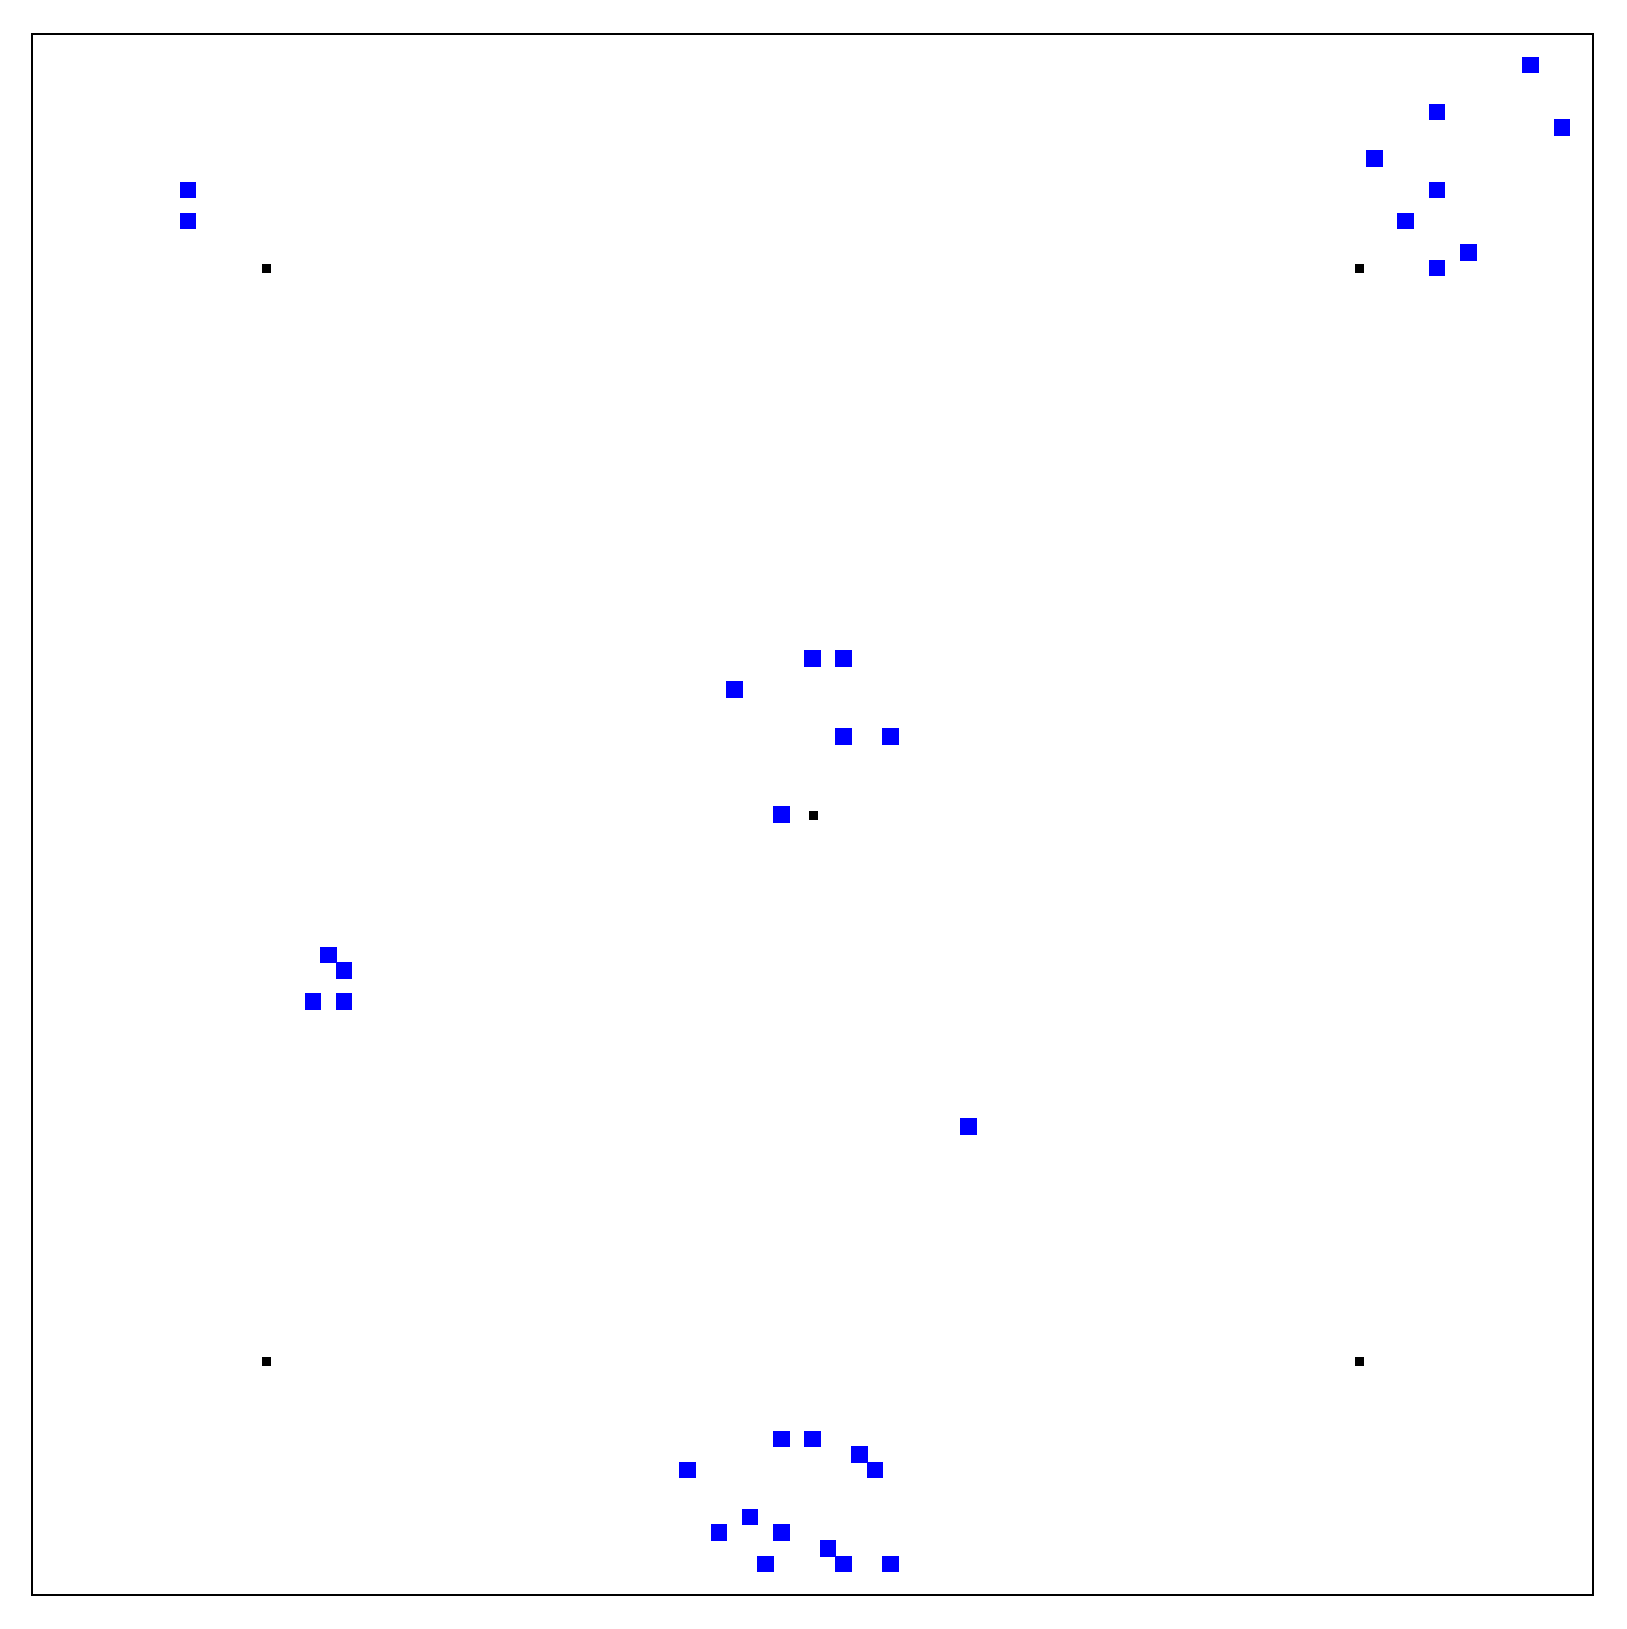
\includegraphics[width=0.5\textwidth]{img/rooms/fullroom.eps}}
  \subfloat[EmptyRoom]{\label{fig:emptyroom}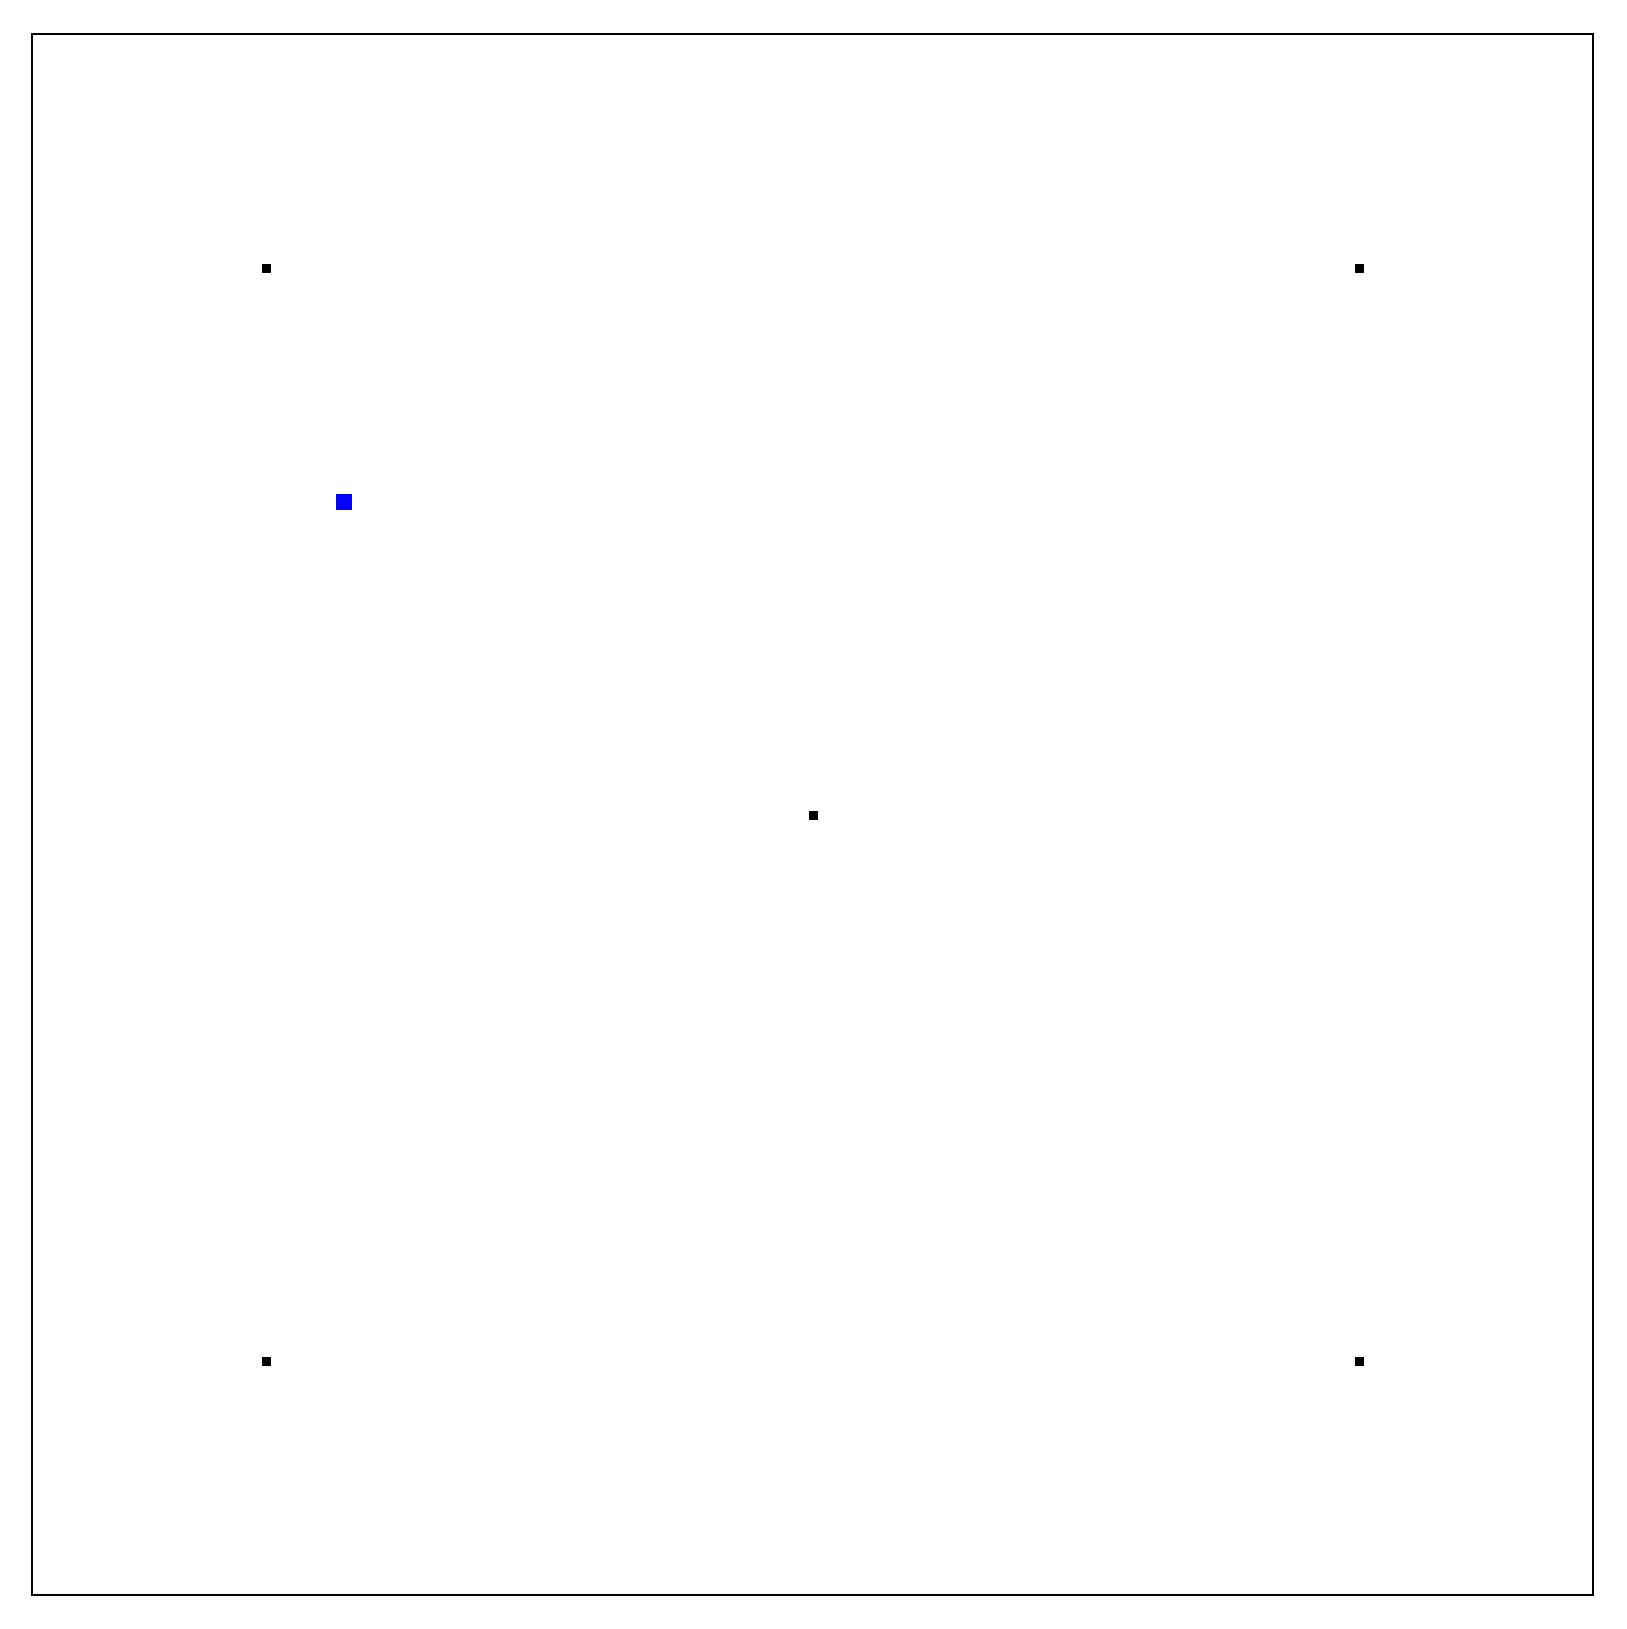
\includegraphics[width=0.5\textwidth]{img/rooms/emptyroom.eps}}
  \caption{Jednoduch� m�stnosti}
  \label{fig:simlpe-rooms}
\end{figure}

\begin{figure}
  \centering
  \subfloat[Corridor]{\label{fig:corridor}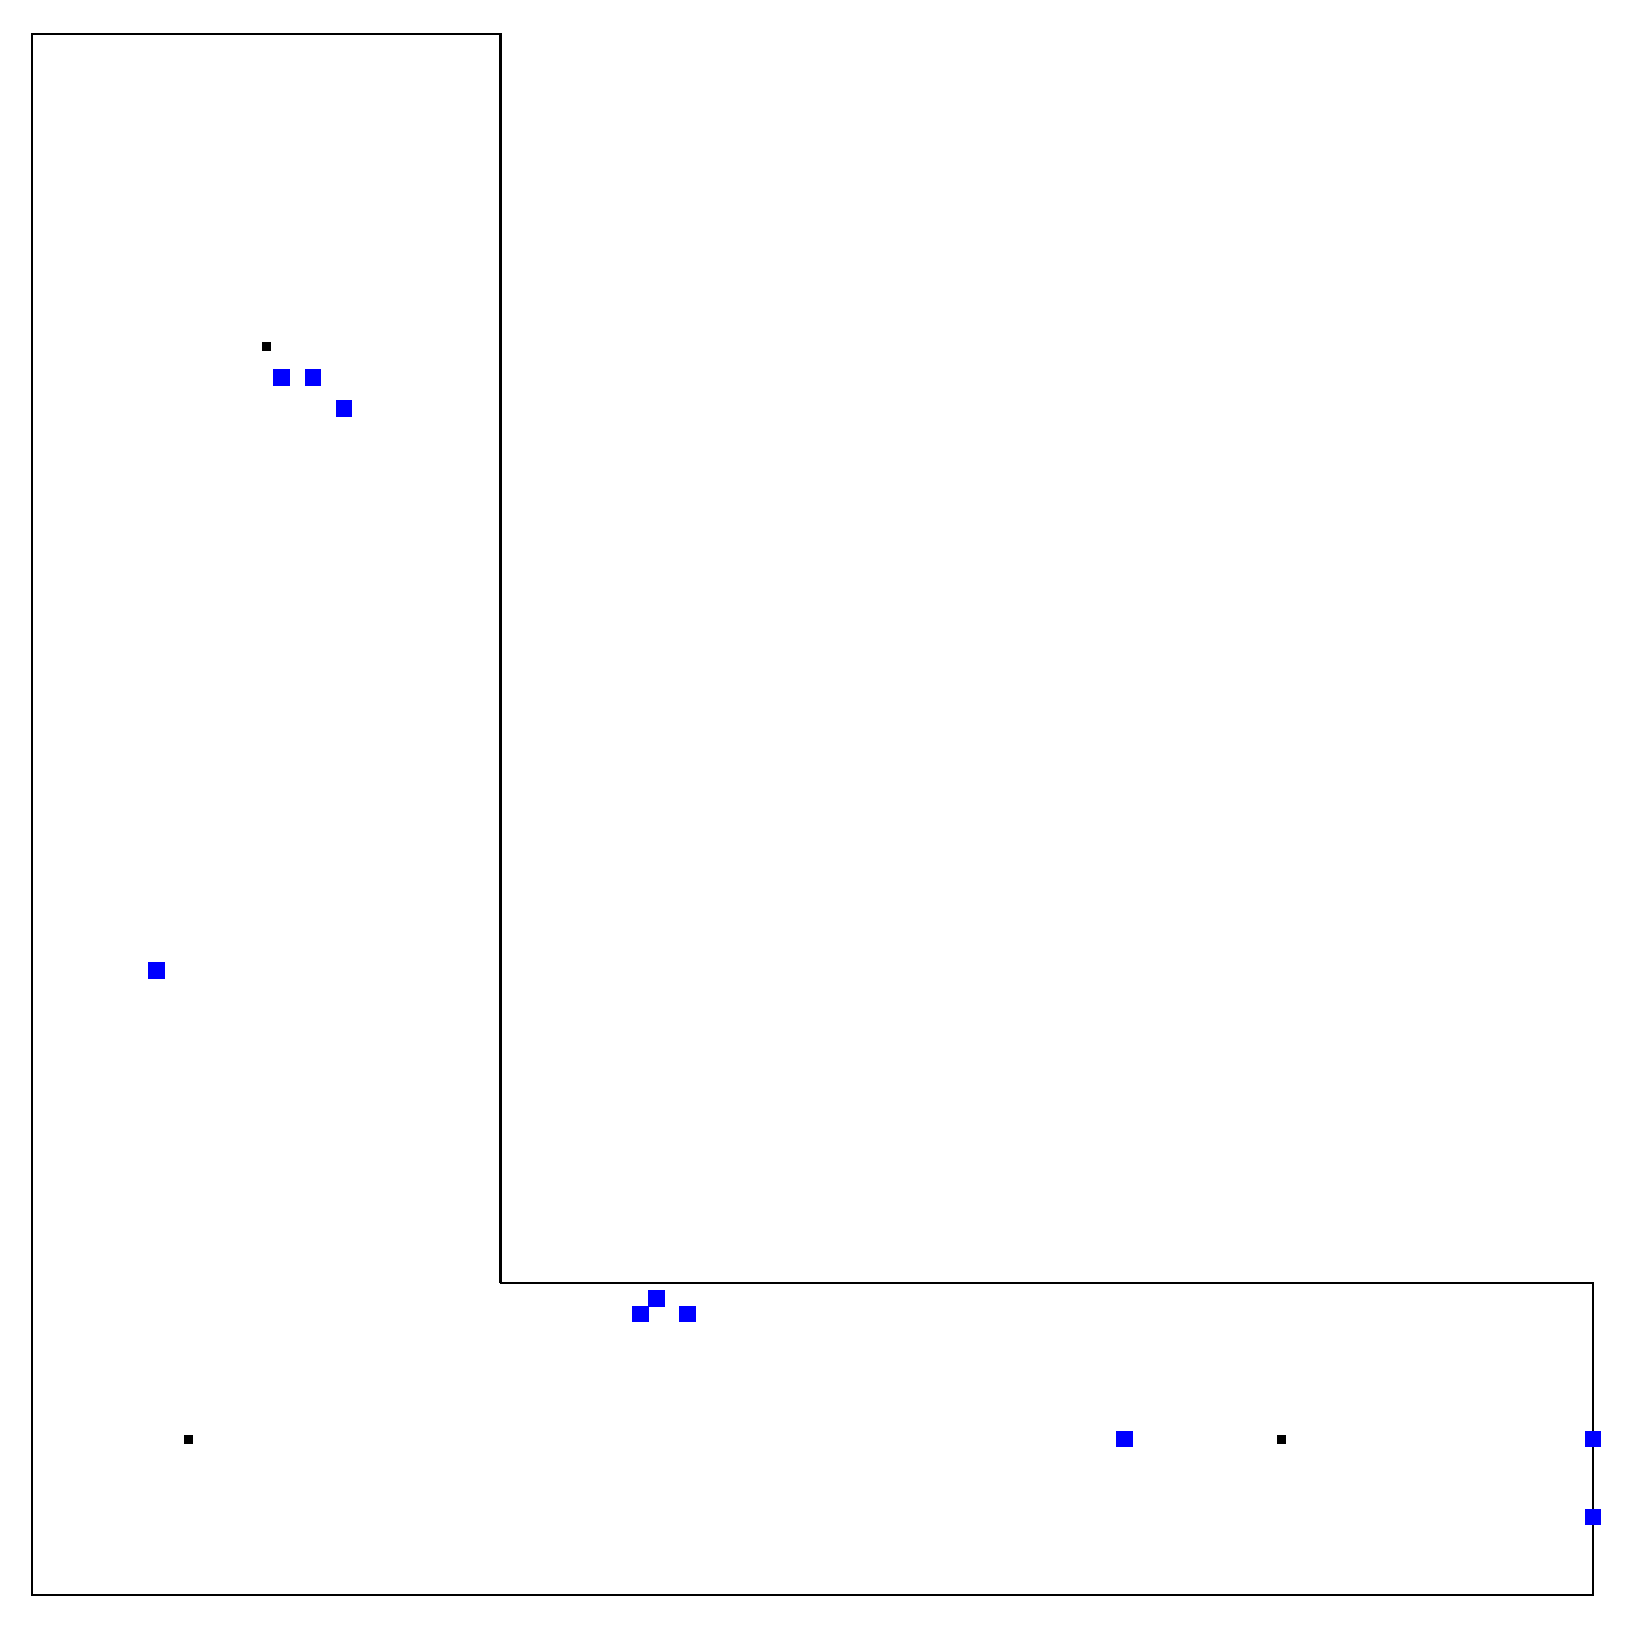
\includegraphics[width=0.5\textwidth]{img/rooms/corridor.eps}}
  \subfloat[Lobby]{\label{fig:lobby}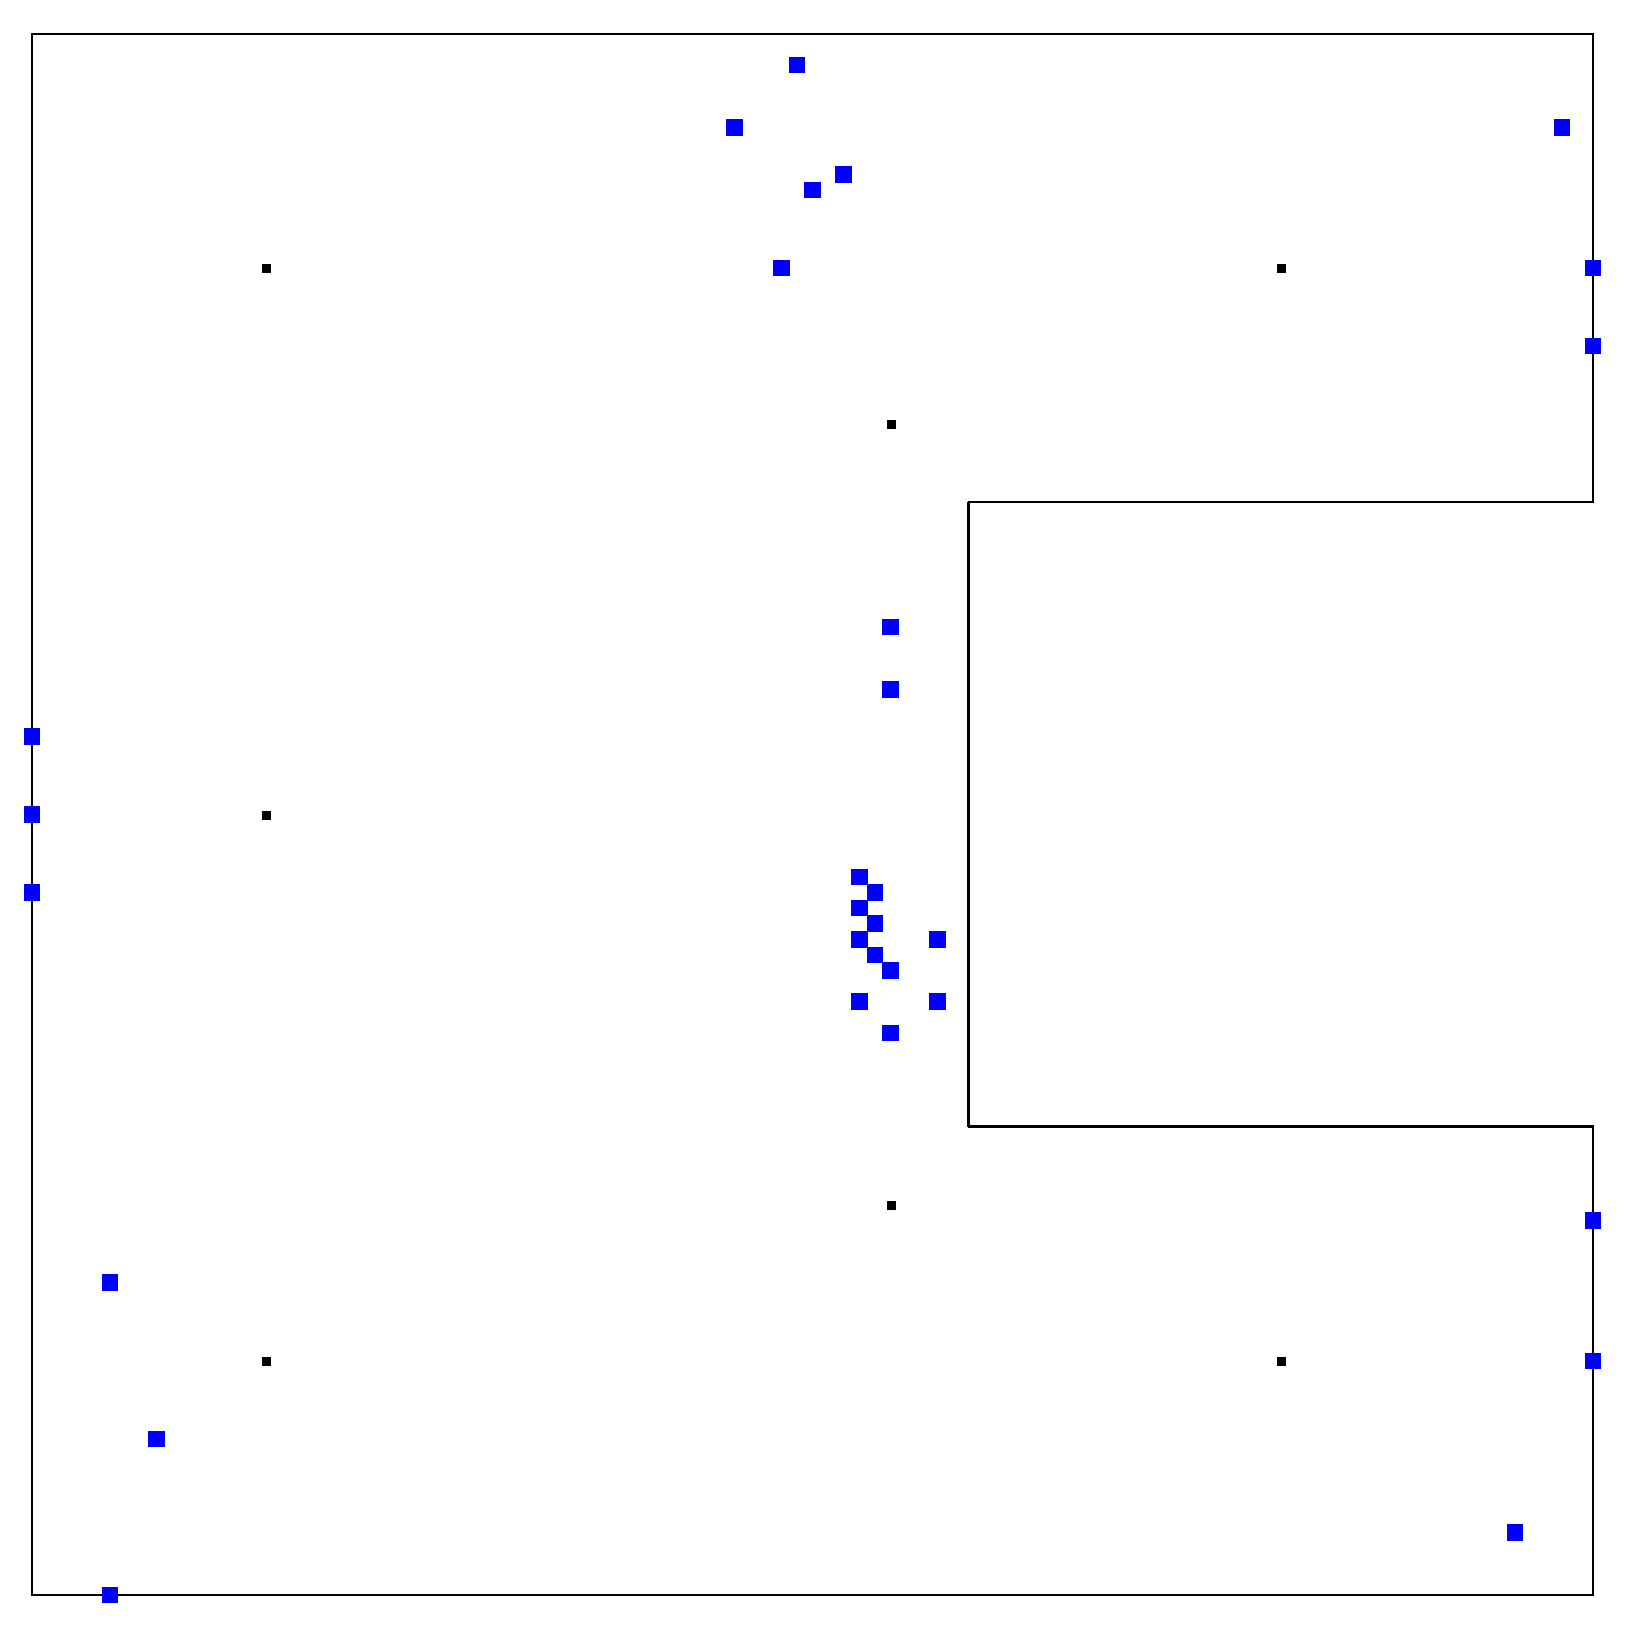
\includegraphics[width=0.5\textwidth]{img/rooms/lobby.eps}}
  \caption{Slo�it�j�� m�stnosti}
  \label{fig:advanced-rooms}
\end{figure}

\begin{figure}
  \centering
  \subfloat[CrazyRoom]{\label{fig:crazyroom}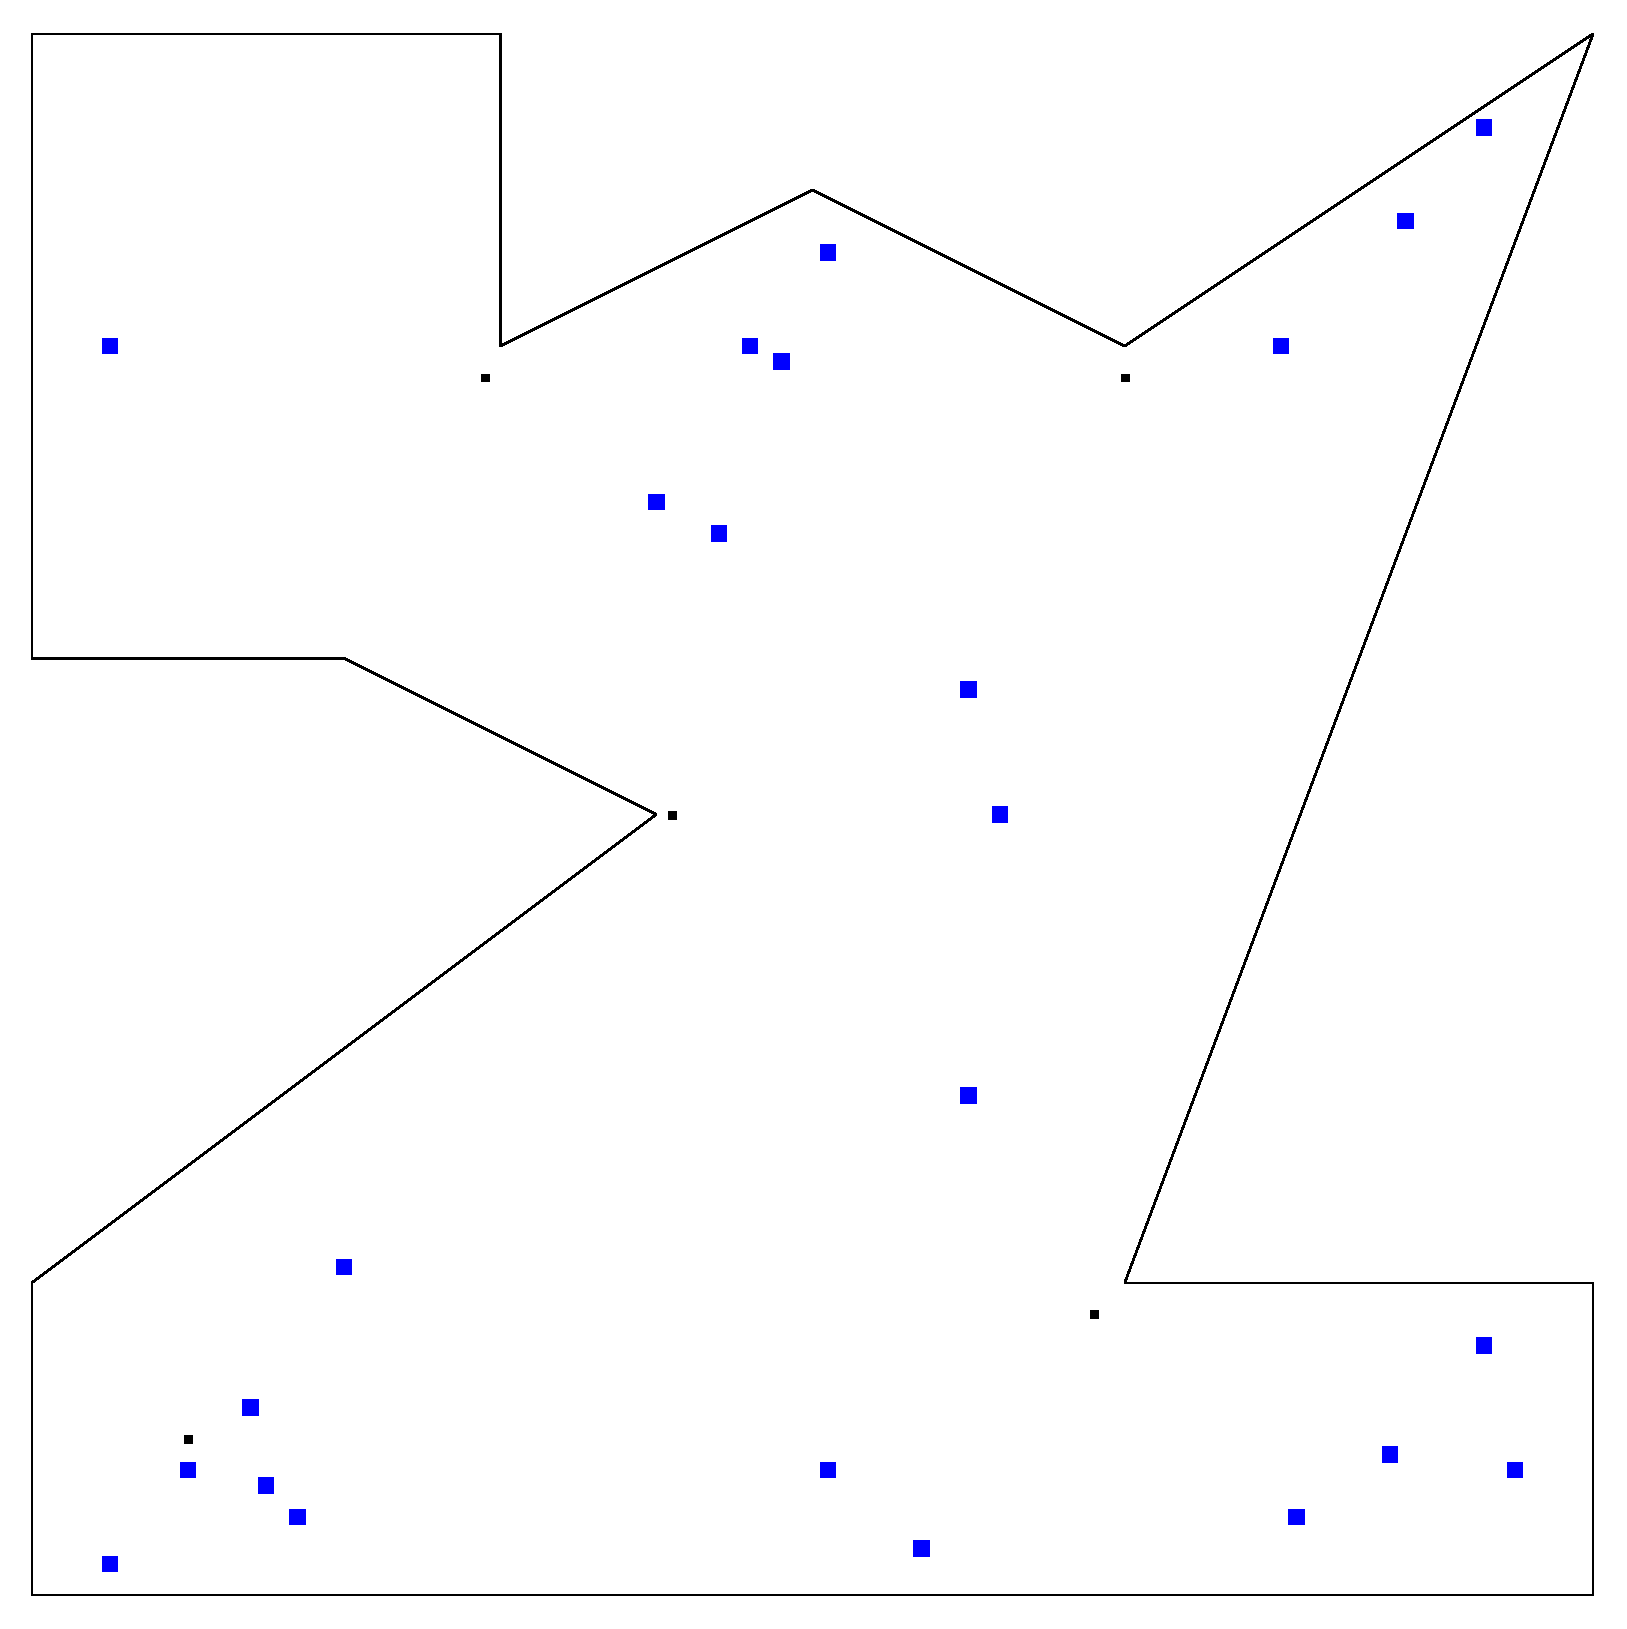
\includegraphics[width=0.5\textwidth]{img/rooms/crazyroom.eps}}
  \subfloat[SmallRoom]{\label{fig:smallroom}\includegraphics[width=0.5\textwidth]{img/rooms/smallroom.eps}}
  \caption{Slo�it�j�� m�stnosti}
  \label{fig:advanced-rooms2}
\end{figure}

\begin{figure}
  \centering
  \subfloat[HeapRoom]{\label{fig:heaproom}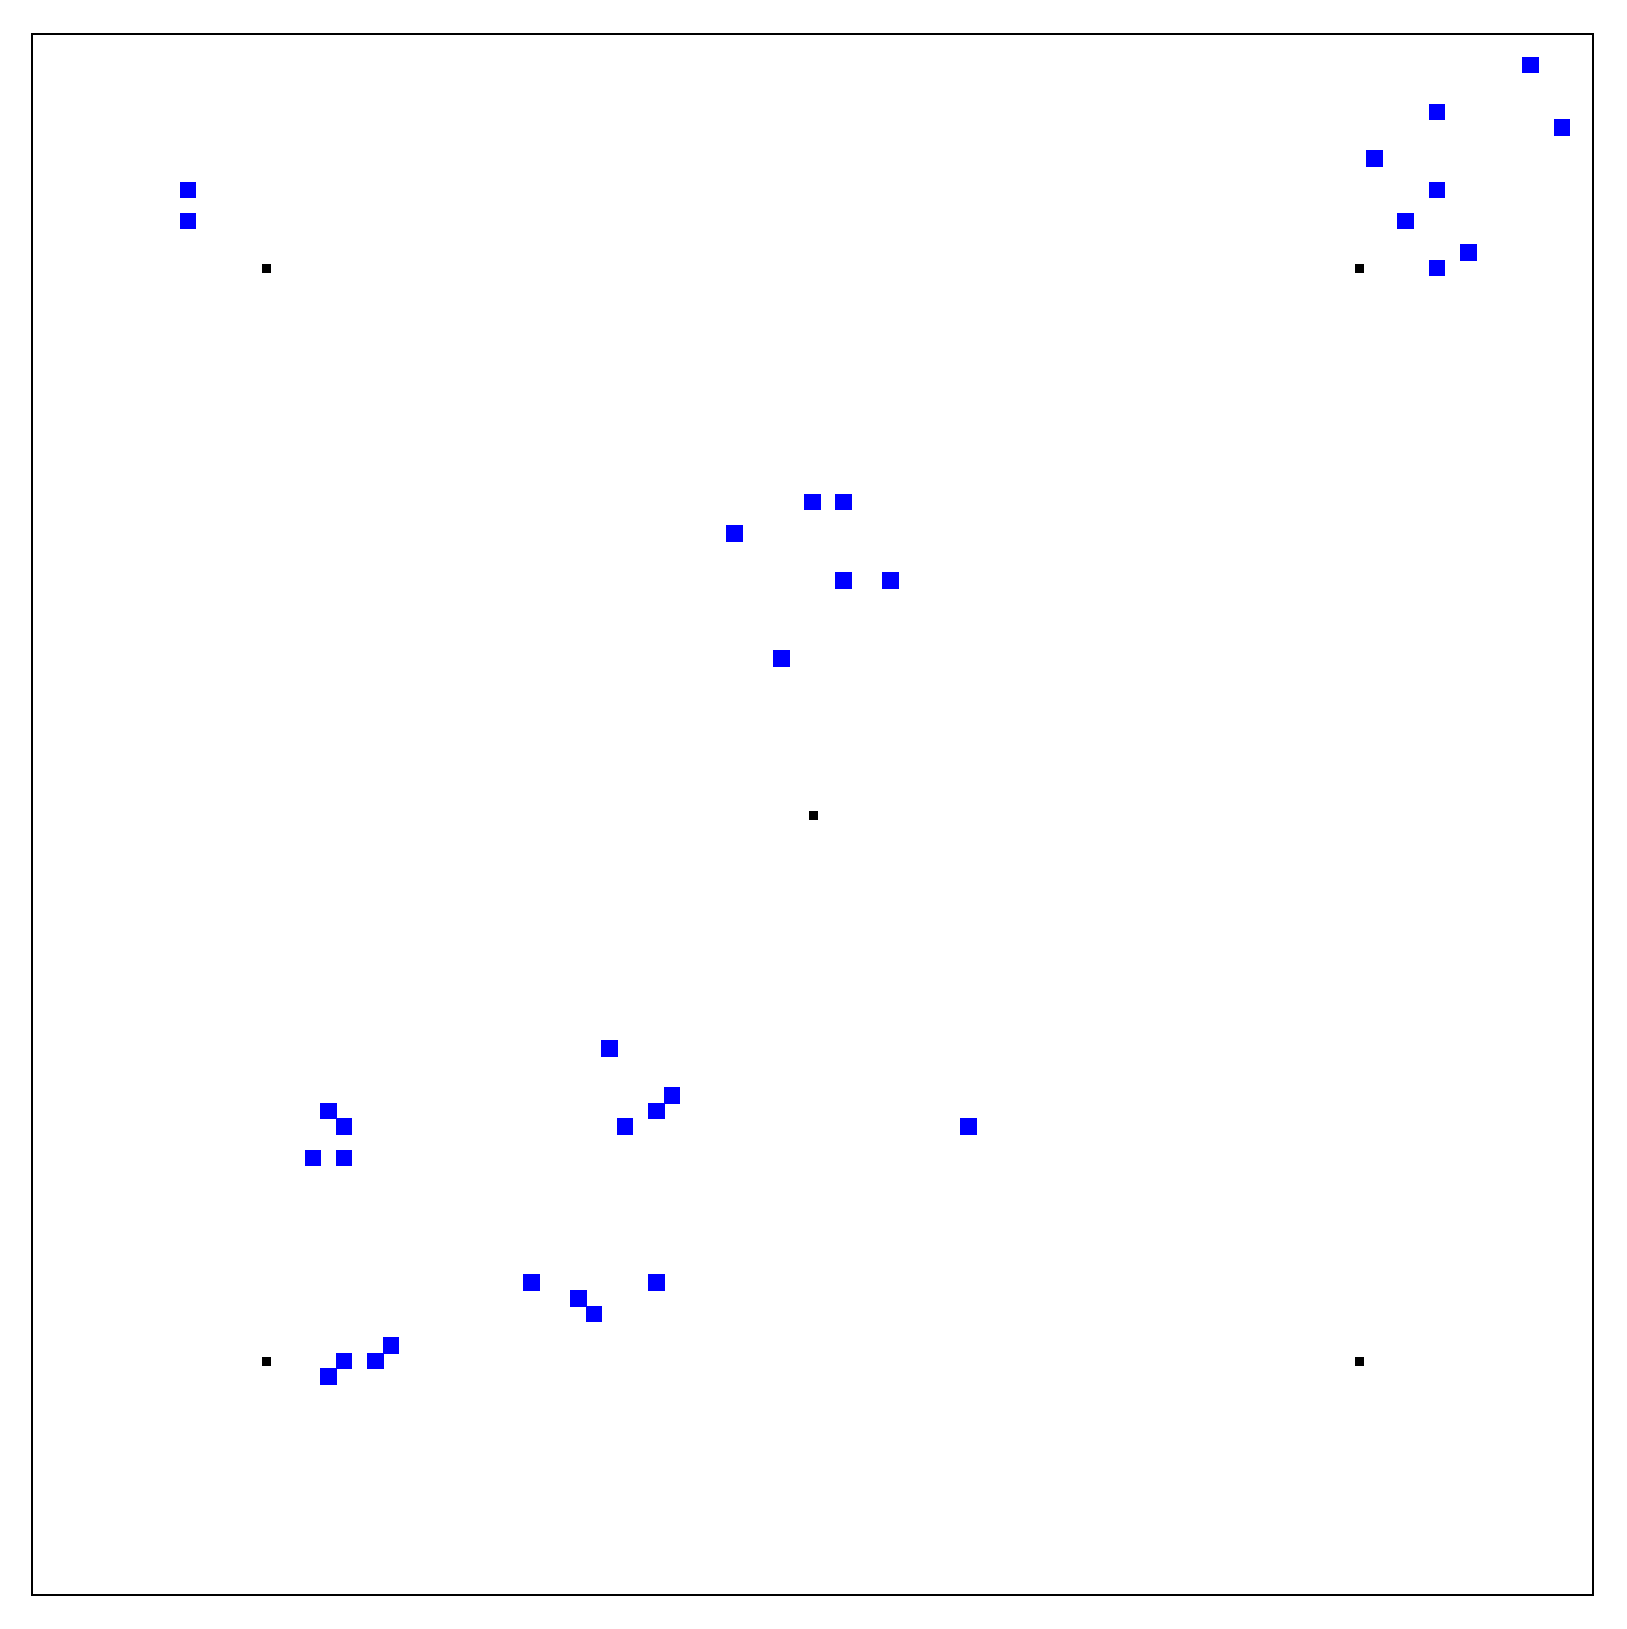
\includegraphics[width=0.5\textwidth]{img/rooms/heaproom.eps}}
  \subfloat[HeapLineRoom]{\label{fig:heaplineroom}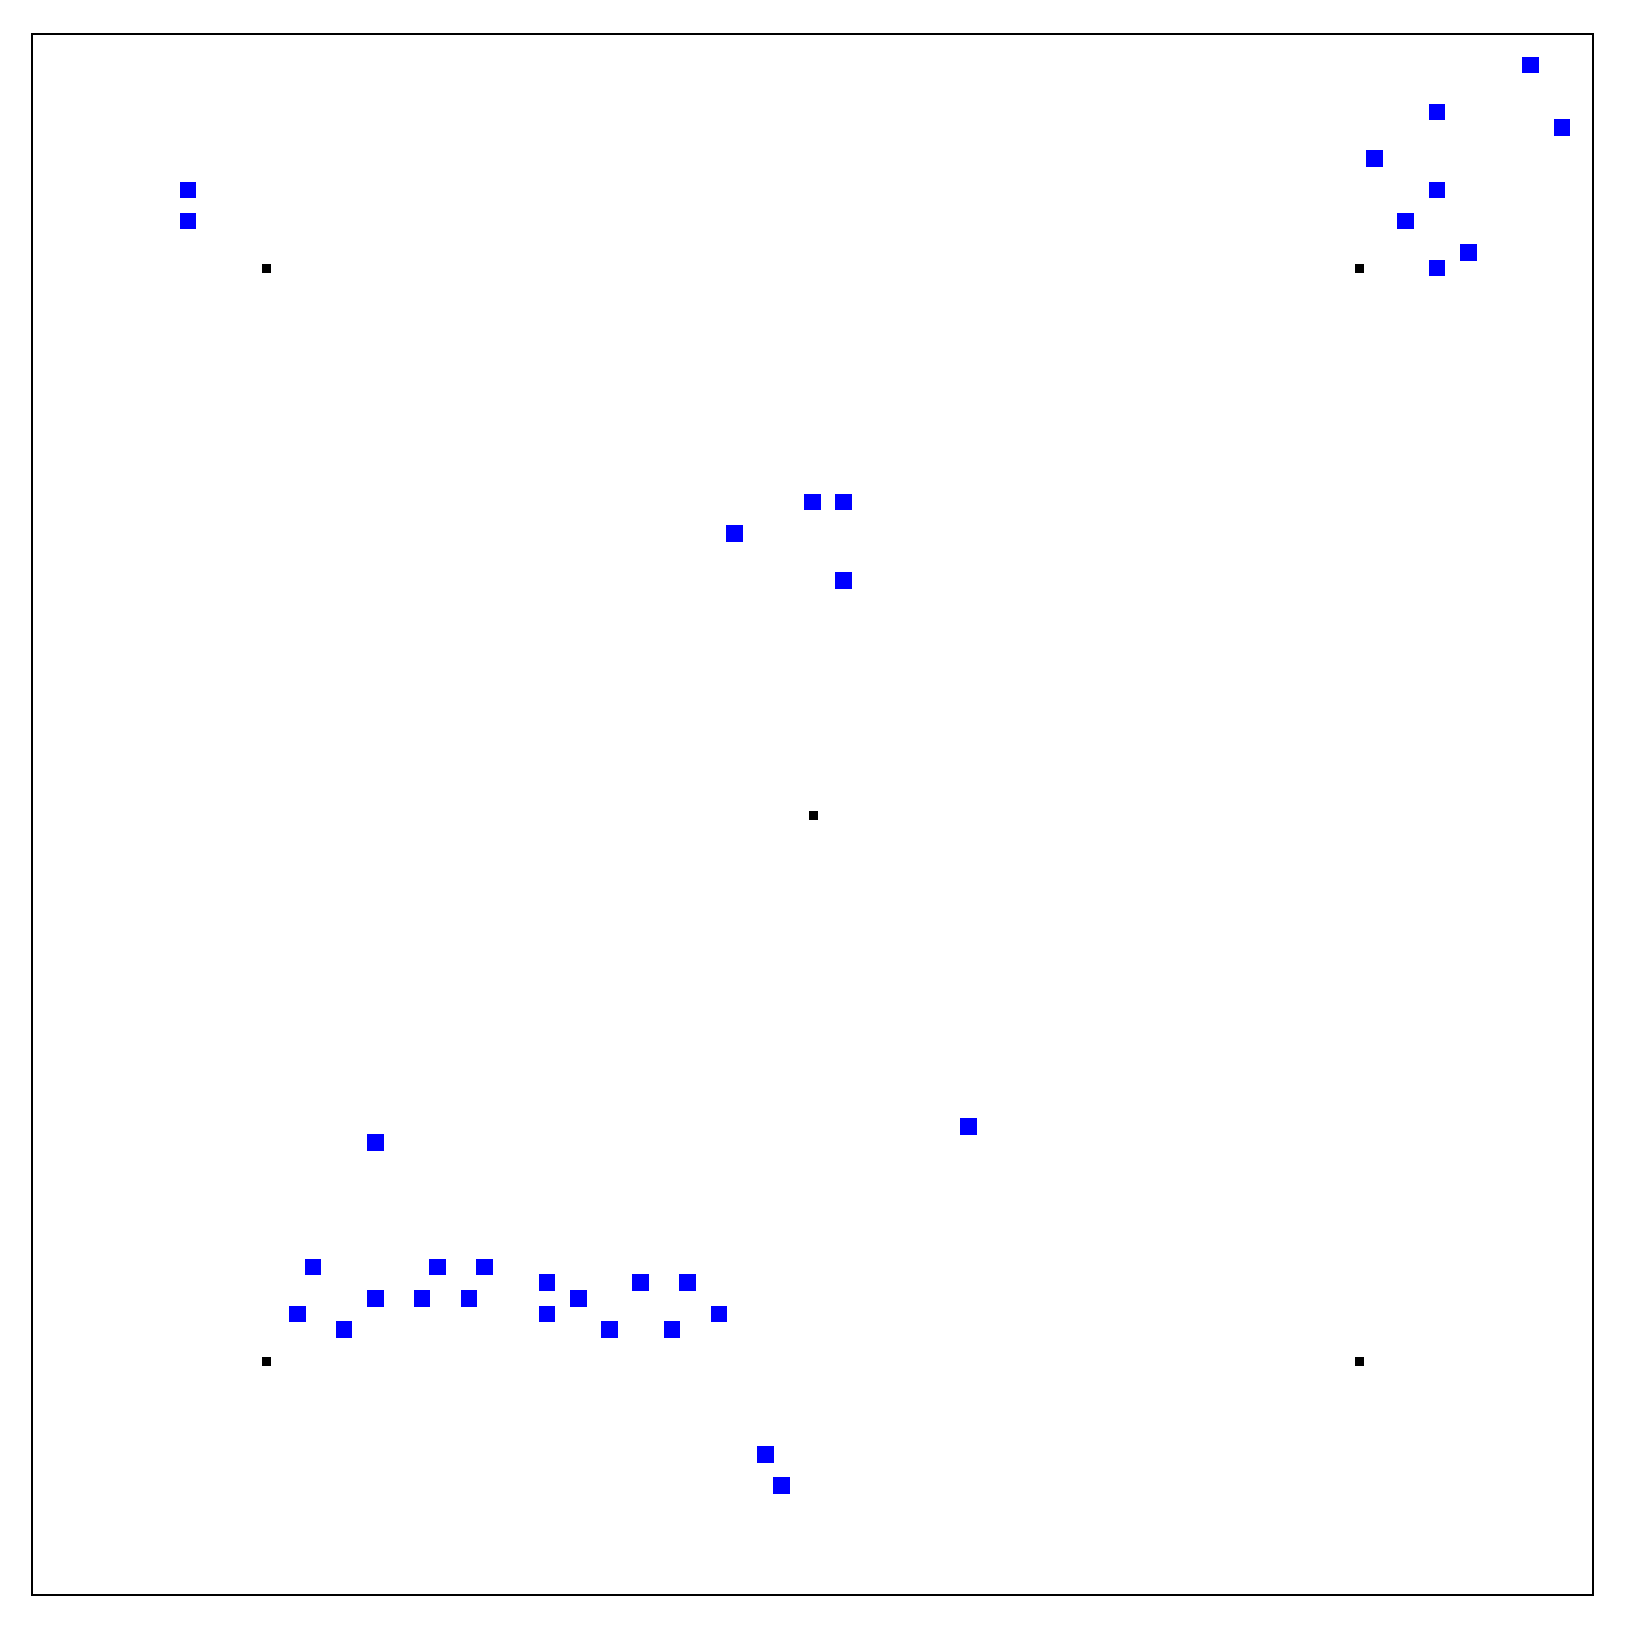
\includegraphics[width=0.5\textwidth]{img/rooms/heaplineroom.eps}}
  \caption{M�stnosti pro testov�n� hierarchie modelu a vytv��en� m�st}
  \label{fig:heaprooms}
\end{figure}

\begin{figure}
  \centering
  \subfloat[Krok 0]{\label{fig:switchroom-1}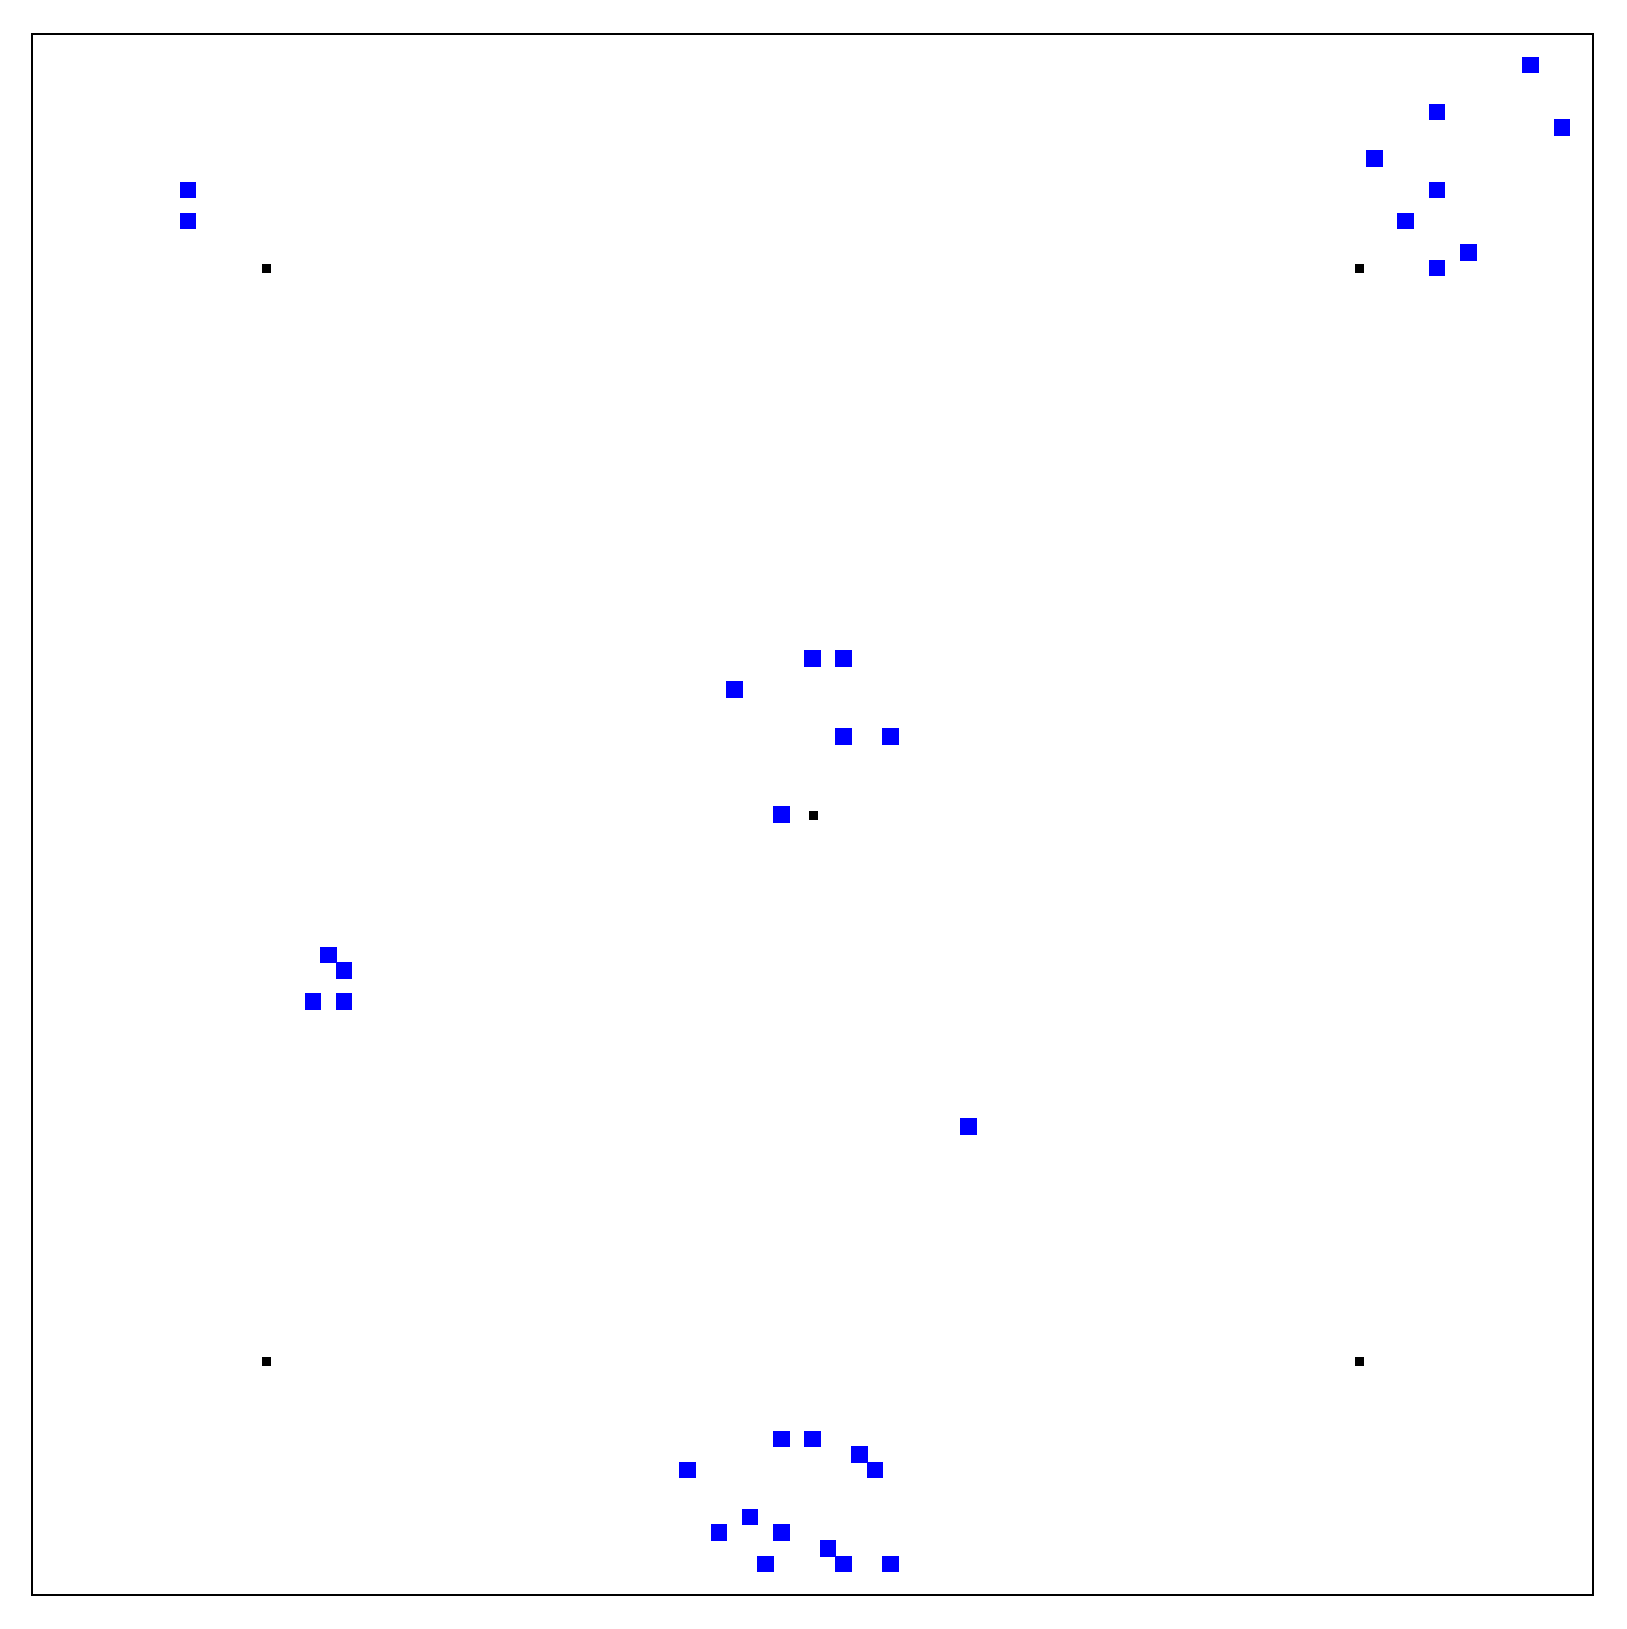
\includegraphics[width=0.4\textwidth]{img/rooms/switchroom-1.eps}}
  \quad
  \subfloat[Krok 1500]{\label{fig:switchroom-2}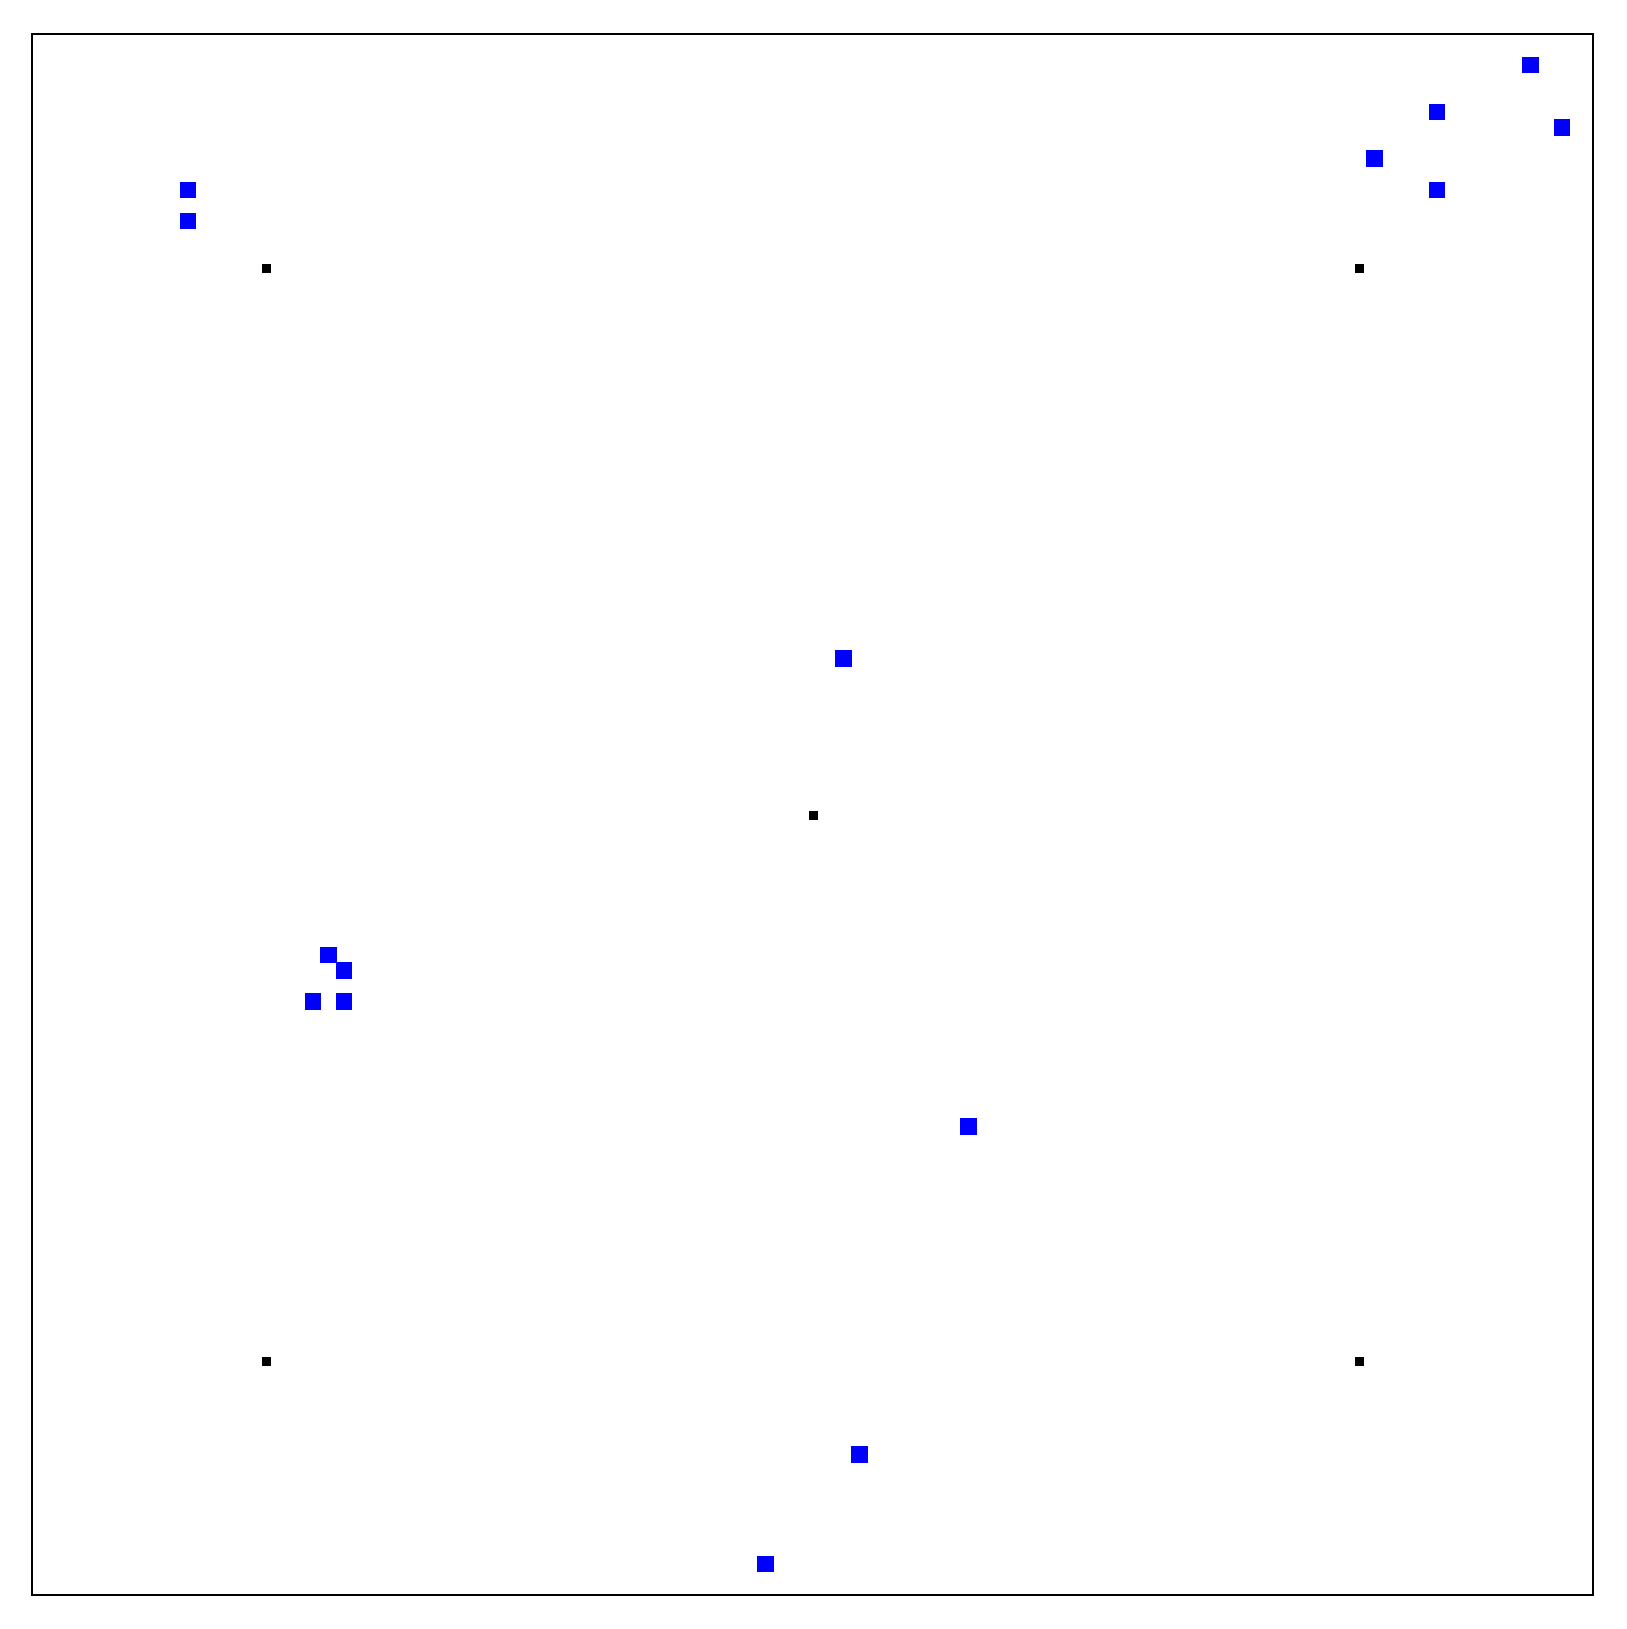
\includegraphics[width=0.4\textwidth]{img/rooms/switchroom-2.eps}}
  \quad
  \subfloat[Krok 4000]{\label{fig:switchroom-3}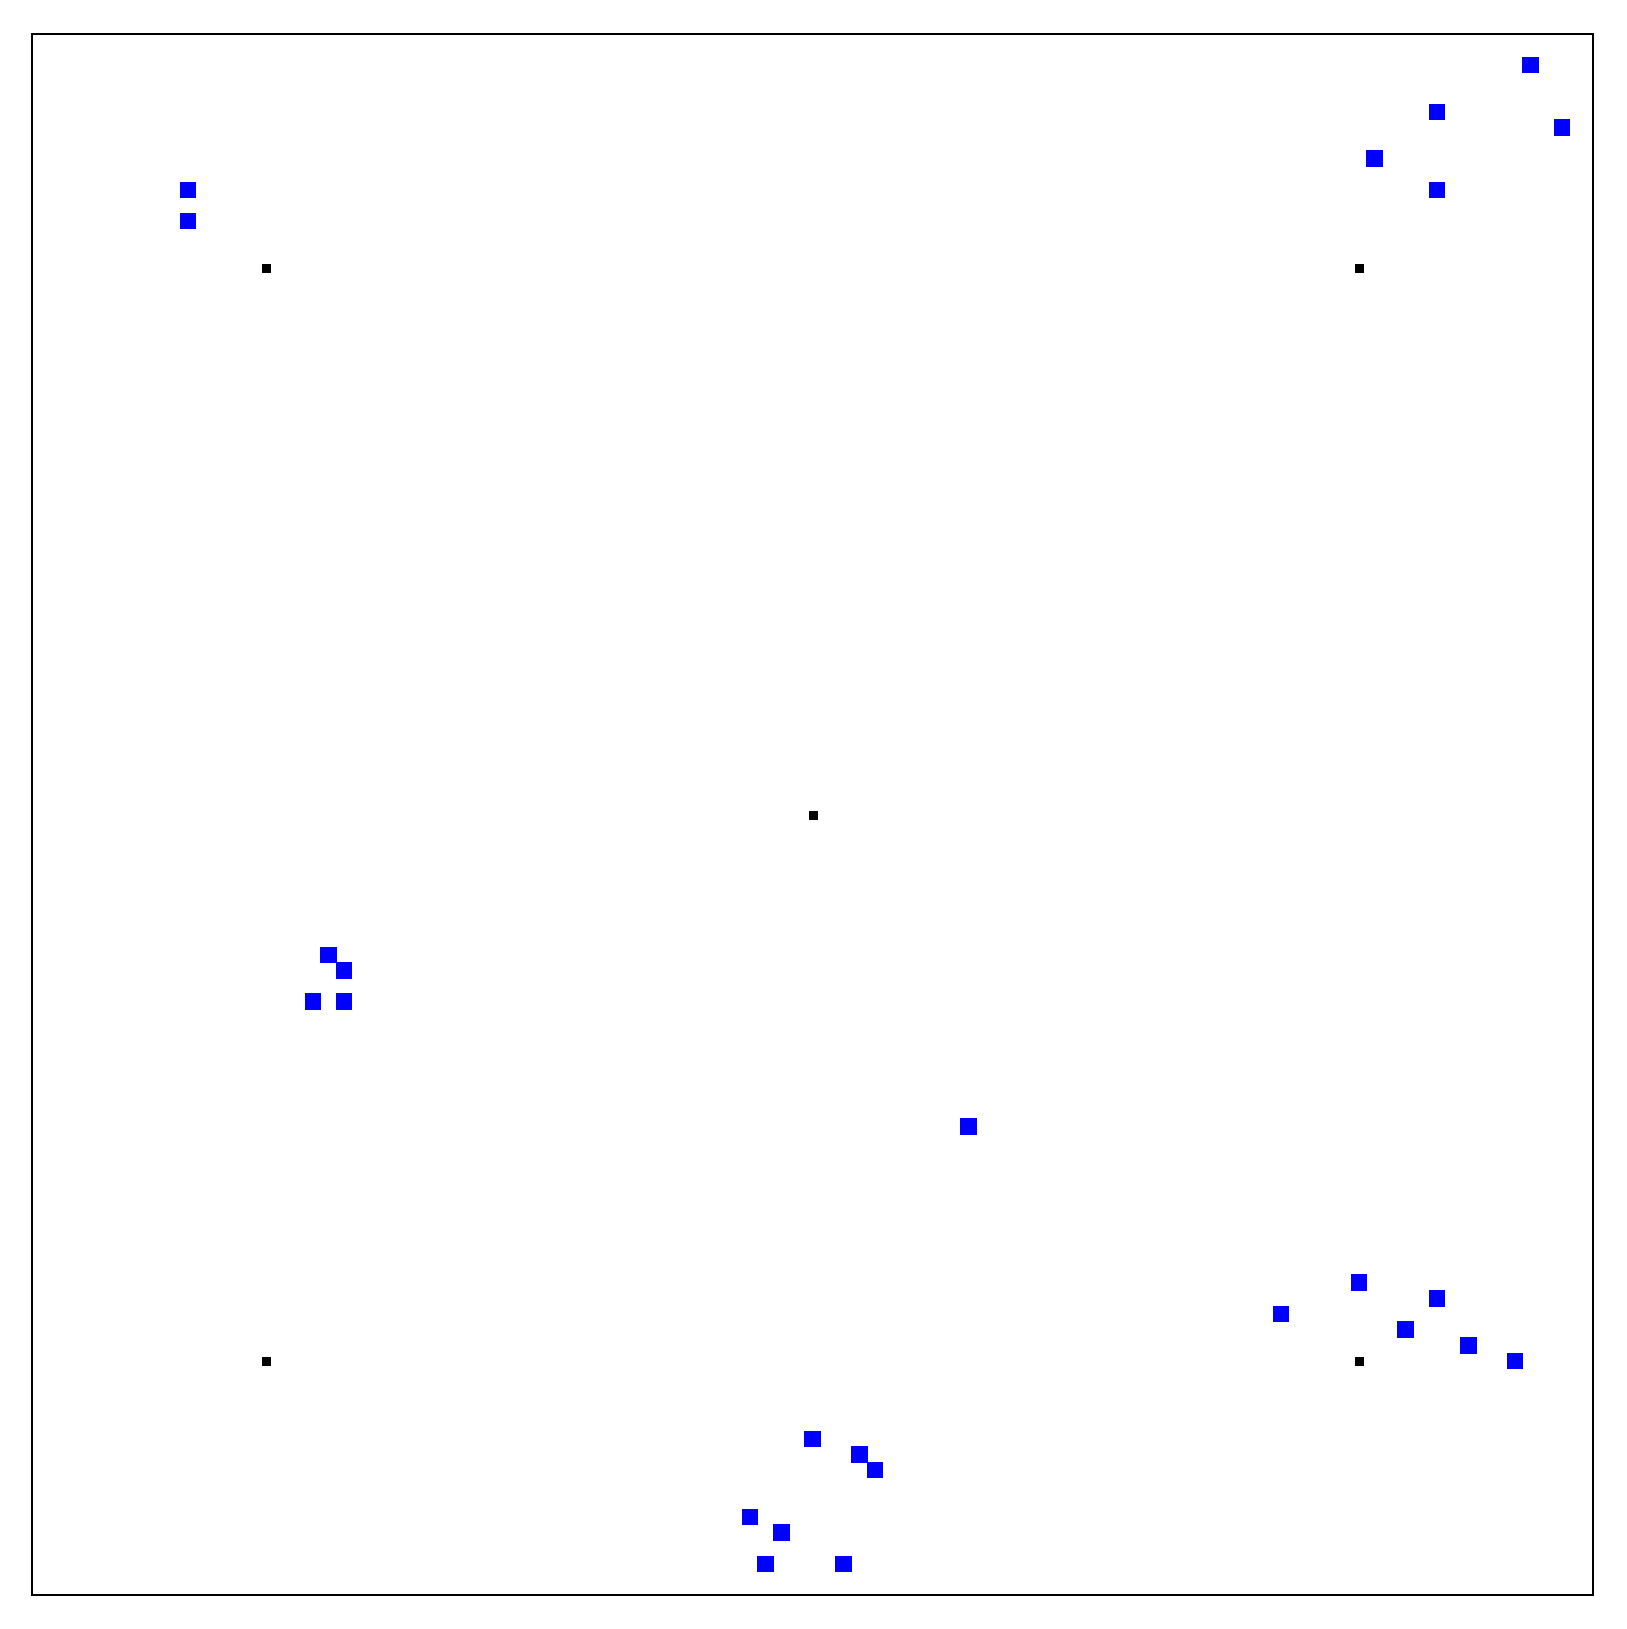
\includegraphics[width=0.4\textwidth]{img/rooms/switchroom-3.eps}}
  \caption{M�stnost SwitchRoom a jej� prom�ny v �ase}
  \label{fig:switchroom}
\end{figure}


\chapter{Parametry modelu}


\begin{table}[h!]
\begin{center}
\begin{tabular}{|l|l|r|r|}\hline

\param{Maxim�ln� krok agenta} & \texttt{MaxAgentMove} & 10 & 2 - 20 \\
\hline

\param{Velikost waypointu} & \texttt{WayPointArea} & 10 & 5 - 20 \\
\hline

\param{Odchylka waypointu} & \texttt{WayPointNoise} & 10 & 0 - 20 \\
\hline

\param{Velikost percep�n�ho pole} & \texttt{PFSize} & 7 & 5 - 9 \\
\hline

\param{Vzd�lenost nutn� k pou�it� p�edm�tu} & \texttt{MapPickUpDistance} & 2 & 1 - 5 \\
\hline

\param{V�choz� atraktivita p�edm�t�} & \texttt{ObjDefaultAttractivity} & 1 & 0,5 - 2 \\
\hline

\end{tabular}
\end{center}
\centering
\caption{Parametry sv�ta a agenta}
\label{tab:param-svet}
\end{table}




\begin{table}[h!]
\begin{center}
\begin{tabular}{|p{6cm}|l|l|l|}\hline


\param{Efekt zpozorov�n� p�edm�tu} & \texttt{TrainEffectNoticed} & 1 & 1 \\
\hline

\param{Efekt zpozorov�n� p�edm�tu znovu} & \texttt{TrainEffectNoticedAgain} & 0,3 & 0,1 - 0,5 \\
\hline

\param{Efekt pou�it� p�edm�tu} & \texttt{TrainEffectUsed} & 3 & 1 - 10 \\
\hline

\param{Efekt nalezen� p�edm�tu} & \texttt{TrainEffectFound} & 2 & 1 - 3 \\
\hline

\param{Efekt nenalezen� p�edm�tu} & \texttt{TrainEffectNotFound} & -1 & -1 \\
\hline

\param{Maxim�ln� d�lka atomick� akce, pokud je del��, provede prostorov� pam� v�ce krok�} & \texttt{SMUpdateMaxDuration} & 100 & 10 - 10000 \\
\hline

\param{Dosah u�en�} & \texttt{SMTrainRange} &  10 & 10 - 20 \\
\hline

\param{Po��te�n� napln�nost uzlu} & \texttt{MemObjIntenseToNewNode} & 1 & 1 - 5 \\
\hline

\param{M�ra zapom�n�n� pam�ov�ch stop p�edm�t�} & \texttt{MemObjIntensityFadeOut} &   0,01 & 0,001 - 0,1 \\
\hline

\param{M�ra zapom�n�n� vazeb mezi uzly a pam�ov�mi stopami} & \texttt{LinkMemObjToNodeFadeOut} & 0,005 & 0,001 - 0,1 \\
\hline

\end{tabular}
\end{center}
\centering
\caption{Parametry pam�ti na p�edm�ty}
\label{tab:param-pametpredmety}
\end{table}






\begin{table}[h!]
\begin{center}
\begin{tabular}{|l|l|r|r|}\hline

\param{Hustota mapy} & \texttt{ELDensity} & 10 & 10 \\
\hline

\param{Po��te�n� odchylka mapy} & \texttt{ELCreateNoise} & 3 & 1 - 5 \\
\hline

\param{Rychlost kles�n� napln�nosti} & \texttt{ELNodeUsageFadeOut} & 0,005 & 0,001 - 0,01 \\
\hline

\param{Dosah p�ita�livosti} & \texttt{ELGravityRange} & 20 & 10 - 30 \\
\hline

\param{S�la p�ita�livosti} & \texttt{ELGravityCoef} & 1 & 0,2 - 3 \\
\hline

\param{Dosah odpudivosti} & \texttt{ELAntigravityRange} & 20 & 10 - 30 \\
\hline

\param{S�la odpudivosti} & \texttt{ELAntigravityCoef} &  8 & 4 - 20 \\
\hline

\param{Vliv napln�nosti} & \texttt{ELAGUsageCoef} & 0,8 & 0,4 - 1 \\
\hline

\param{Limit pohybu uzlu} & \texttt{MaxELNodeMove} &  4 & 1 - 5 \\
\hline

\param{Vliv vjemu} & \texttt{EPCreateEnergy} &  140 &  100 - 200\\
\hline

\param{Odchylka vytvo�en� uzlu} & \texttt{ELNodeAddNoise} &  2  & 1 - 5 \\
\hline

\param{M�ra slabnut� stopy vjemu} & \texttt{EPFadeCoef} & 0,5  & 0 - 0,9 \\
\hline

\param{Limit zmizen� stopy vjemu} & \texttt{EPFadeLimit} &  10 & 1 - 20 \\
\hline

\param{M�ra zapom�n�n� uzl�} & \texttt{ELForgetNodeRate} & 5 & 1 - 10 \\
\hline

\param{Po�et opakov�n�} & \texttt{ELDeleteNodeReTrainCount} & 20 & 10 - 50 \\
\hline

\param{Velikost okol�} & \texttt{ELDeleteNodeReTrainRange} & 20 & 5 - 40 \\
\hline

\param{Rychlost r�stu $\varrho$} & \texttt{ELAGAddCoef} &  3 & 1 - 5 \\
\hline

\param{Rychlost kles�n� $\varrho$} & \texttt{ELAGFadeOut} &  0,1 & 0,01 - 1 \\
\hline

\param{Limit vzniku podm�sta} & \texttt{PlacesAGNeeded} &  1500 & 500 - 5000 \\
\hline

\param{Limit zapomenut� m�sta} & \texttt{PlacesAGMin} &  500 & 100 - 200 \\
\hline

\param{Rychlost r�stu intenzity} & \texttt{PlacesAGGrow} &  0,1 & 0,01 - 0,5 \\
\hline

\param{Rychlost kles�n� intenzity} & \texttt{PlaceAGFadeOut} &  0,5 & 0,1 - 1 \\
\hline

\param{Pohyblivost m�st} & \texttt{PlaceMoveCoef} &  0,02 & 0,01 - 0,5 \\
\hline

\end{tabular}
\end{center}
\centering
\caption{Parametry gravita�n�ho modelu vrstvy uzl�}
\label{tab:param-el}
\end{table}

\chapter{U�ivatelsk� dokumentace}

\section{Instalace}
Nejd��ve je t�eba nainstalovat pot�ebn� knihovny:
\begin{CompactItemize}
\item interpetor jazyka Python 
\item grafick� knihovna GTK+
\item knihovna NumPy\footnote{pro n�stroj \texttt{plotter.py}\label{fn:repeat}} a Matplotlib\footref{fn:repeat}
\item knihovna .Net Framework 3.5\footnote{pro n�stroj \texttt{statter.exe}}
\end{CompactItemize}



Tyto knihovny jsou na p�ilo�en�m CD.
Aplikaci je pak nutn� zkop�rovat na pevn� disk.
\\

\section{Ovl�d�n� aplikace}
Aplikace se spou�t� hlavn�m souborem \texttt{mainGUI.py}, lze ji ovl�dat pomoc� menu.
Menu \texttt{World} umo��uje zobrazit p�ehled afordanc�, typ� p�edm�t� a p�edm�t�. Menu \texttt{Quit} ukon�� aplikaci.
M��e pracovat ve dvou m�dech: interaktivn�m a testovac�m.
\\

Interaktivn� m�d lze spustit vybr�n�m jm�na testovac�ho sv�ta v polo�ce menu \texttt{Start}.
Aplikace pak spust� simulaci jedn� m�stnosti. Stav sv�ta, agenta a prostorov� mapy, je zobrazen v okn� aplikace.
Simulaci je mo�n� pozastavit (\texttt{Pause}), znovu spustit (\texttt{Resume}) a zru�it (\texttt{Stop}).
V pr�b�hu simulace lze zobrazitt informace o n�kter�ch objektech sv�ta a prostorov� mapy:
kliknut�m na p�edm�t �i uzel prostorov� mapy se zobraz� mal� okno s podrobn�mi �daji. Pro tyto ��ely je vhodn� simulaci pozastavit.
V pr�b�hu aplikace ukl�d� data do adres��e \texttt{../../exs}.
\\

Testovac� m�d lze spust�m polo�kou \texttt{TestAll} menu \texttt{Start}.
Aplikace spust� postupn� v�echny dostupn� testy. Vytvo�� adres�� \texttt{../../tests/yyyy-mm-dd--hh-mm-ss/}.
Do tohoto adres��e zkop�ruje sv� aktu�ln� nastaven� - soubor \texttt{Global.py}
Pro ka�d� testovan� sv�t vytvo�� v tomto adres��i podadres�� \texttt{/nazev-sveta} a do n�j ukl�d� data.
Stav sv�ta a prostorov� mapy nen� zobrazen v okn� aplikace, ale je ukl�d�n do soubor� ve form�tu PNG.
V okn� aplikace jsou zobrazeny jen z�kladn� informace o pr�b�hu testu.
V tomto m�du je aplikace optimalizov�na na v�kon a nelze ji ukon�it pomoc� menu \texttt{Quit}, je nutn� ji zav��t klasick�m tla��tkem Windows: Close v prav�m horn�m rohu aplikace.
\\


V obou m�dech jsou ukl�d�na podrobn� data do textov�ch soubor�. Tato data je mo�n� pomoc� n�stroj� \texttt{statter.exe} a \texttt{plotter.py} vizualizovat.
Test dev�ti sv�t� s 5000 kroky simulace m��e vygenerovat a� 3GB dat.
Nastaven� aplikace m� dv� ��sti:

\begin{CompactItemize}
\item nastaven� parametr� modelu - soubor \texttt{Enviroment/Global.py}
\item ur�en� testovac�ch sv�t� - soubor \texttt{Config/Config.py} a soubory sv�t� v adres��i \texttt{Config}
\end{CompactItemize}

V�znam parametr� v souboru \texttt{Global.py} je uveden v koment���ch a v p��loze B.
\\

\section{V�stupn� data a jejich vizualizace}

V�stupem aplikace jsou n�sleduj�c� soubory:
\begin{description}
\item[PIL000000.png--PIL999999.png] \hfill \\
  obr�zky stavu sv�ta a prostorov� mapy v ka�d�m kroku simulace
\item[visibilityobjectheatmap.png] \hfill \\
  obr�zek stavu v posledn�m kroku simulace v�etn� nau�enosti p�edm�tu
\item[data-scenario.txt] \hfill \\
  agent�v sc�n��
\item[data-nc.txt] \hfill \\
  po�et uzl�
\item[data-elnode-status.txt] \hfill \\
  stav v�ech uzl� v ka�d�m kroku
\item[data-place-status.txt] \hfill \\
  stav v�ech m�st v ka�d�m kroku
\item[data-rememberinfo.txt] \hfill \\
  chyba mapy pro ka�d� objekt ka�d� 10-t� krok  
\item[data-elnodeheatmap.txt] \hfill \\
  mapa rozlo�en� uzl� po skon�en� simulace s jejich napln�nost�
\item[data-elnodeheatmapag.txt] \hfill \\
 mapa rozlo�en� uzl� po skon�en� simulace s jejich mno�stv�m odpudivosti
\item[data-objheatmap.txt] \hfill \\
  mapa rozlo�en� p�edm�t� po skon�en� simulace s jejich nau�enost�
\item[log.txt] \hfill \\
  podrobn� informace o pr�b�hu simulace  
\end{description}

Data v textov�ch souborech je mo�n� vizualizovat pou�it�m n�stroj� \texttt{statter.exe}\footnote{
je pot�eba pouze, pokud u�ivatel chce vid�t podrobn� informace o stavu uzl� prostorov� mapy v pr�b�hu simulace} a \texttt{plotter.py}.
Oba n�stroje pracuj� tak, �e po spu�t�n� projdou aktu�ln� adres�� a rekurzivn� v�echny podadres��e a zpracuj� v�echny nalezen� soubory se spr�vn�m jm�nem.
\\

N�stroj statter.exe spo��t� pr�m�rn�, minim�ln� a maxim�ln� hodnoty dat v souborech
\texttt{data-elnode-status.txt} a \texttt{data-place-status.txt} a ulo�� je do soubor� \texttt{data-elnode-status.stats.txt} a \texttt{data-places-status.stats.txt}.
\\

N�stroj \texttt{plotter.py} na z�klad� textov�ch soubor� vytvo�� grafy a ulo�� je do soubor� ve form�tu PNG.
\\
\chapter{Program�torsk� dokumentace}

Prototypov� aplikace je naps�na v jazyce Python, vyu��v� knihovnu TkInter pro GUI a knihovnu PIL\footnote{Python Imaging Library} k ukl�d�n� dat do grafick�ch soubor�.
Aplikace je rozd�lena do �ty� modul�:

\begin{description}
\item[\texttt{Gui}] - grafick� rozhran� aplikace a grafick� v�stupy
\item[\texttt{Config}] - testovac� sv�ty
\item[\texttt{Enviroment}] - model sv�ta a parametry
\item[\texttt{Agents}] -  model agent a prostorov� mapy
\end{description}

Grafick� rozhran� a ��zen� cel� aplikace a zaji��uje t��da \texttt{Gui.MainWindow}. T��da \texttt{Gui.MapRender} vykresluje stav sv�ta do okna aplikace a do souboru.
Sv�t je reprezentov�n t��dami \texttt{Enviroment.World} a dal��mi t��dami v modulu \texttt{Enviroment}.
T��da \texttt{Enviroment.Global} obsahuje pomocn� metody a v�echny parametry modelu.
\\

Agent je reprezentov�n t��dou \texttt{Agents.Agent}.
T��da \texttt{Intelligence} p�edstavuje jeho \uv{mozek}, obsahuje dal�� t��dy, kter� zaji��uj� ��zen� jeho chov�n�, vn�m�n� a pam�.
\\

Jeden krok simulace je zavol�n� metody \texttt{World.Step()}. Ta provede jeden krok agenta metodou \texttt{Agent.Step()}, popsanou v algoritmu \ref{alg:prog-step}.
Pak metodou \texttt{Map.Step()} spo�it� viditelnost p�edm�t�.
\\

\begin{algorithm}[h!]
\caption{Jeden krok simulace agenta}
\label{alg:prog-step}
\begin{algorithmic}[1]
\State vybr�n� atomick� akce - \texttt{ActionSelector.GetAction()}
\State proveden� akce
\State vn�m�n� viditeln�ch p�edm�t�
\State aktualizace \texttt{PerceptionField}
\State aktualizace \texttt{MemoryArea}
\State aktualizace And-Or stromu akc� v \texttt{ProcessArea} zavol�n�m metody \texttt{ActionSelector.ActionDone()}
\State aktualizace prostorov� mapy: \texttt{SpaceMap} a \texttt{EnergyLayer}
\end{algorithmic}
\end{algorithm}



\begin{table}[h!]
\begin{center}
\begin{tabular}{llcc}\toprule[0.5pt]

Pojem modelu & \texttt{N�zev v implementaci} \\
\midrule[0.4pt]

Sv�t & \texttt{World} \\
M�stnost & \texttt{Map} \\
P�edm�t & \texttt{RealObject} \\
Typ p�edm�tu & \texttt{Object} \\

\midrule[0.1pt]
 
Agent & \texttt{Agent} \\
V�b�r akce & \texttt{ActionSelector} \\
Chytr� akce & \texttt{smart action} \\

\midrule[0.1pt]
 
Zorn� pole & \texttt{ViewCone} \\
Percep�n� filtr & \texttt{PerceptionFilter} \\
Percep�n� pole & \texttt{PerceptionField} \\
Fantom & \texttt{Phantom} \\

\midrule[0.1pt]

Pam�ov� ��st & \texttt{MemoryArea} \\
Pam�ov� fantom & \texttt{MemoryPhantom} \\

\midrule[0.1pt]

Procesn� ��st, And-Or strom akc� & \texttt{ProcessArea} \\
Z�m�r & \texttt{Intetion} \\
�innost & \texttt{Process} \\
Aktivn� z�m�r & \texttt{ExcitedIntention} \\
Aktivn� �innost & \texttt{ExcitedProcess} \\

\midrule[0.1pt]

Prostorov� mapa a pam� na p�edm�ty & \texttt{SpaceMap} \\
Pam�ov� stopa p�edm�tu  & \texttt{MemoryObject} \\
Vazba mezi pam�ovou stopou a uzlem & \texttt{LinkMemoryObjectToNode} \\

\midrule[0.1pt]

Gravita�n� model vrstvy uzl� & \texttt{EnergyLayer} \\
Uzel prostorov� mapy & \texttt{EnergyLayerNode} \\
Napln�nost uzlu & \texttt{EnergyLayerNode.usage} \\
Stopa vjemu & \texttt{EnergyPoint} \\
Intenzita stopy vjemu & \texttt{EnergyPoint.energy} \\
Mno�stv� odpudisvoti & \texttt{AGamount} \\
M�sto & \texttt{Place} \\
Intenzita m�sta & \texttt{Place.slowAGamount} \\

\bottomrule[0.5pt]
\end{tabular}
\end{center}
\centering
\caption{P�enesn� modelu do implementace}
\label{tab:prog-model}
\end{table}

Tabulka \ref{tab:prog-model} popisuje p�enesen� modelu do implementace.
%Soubory \texttt{EpisodicMemory} a \texttt{Emotion} byly p�evzaty od Tom�e Korenka beze zm�ny.
\\

Rychlost aplikace z�v�s� na po�tu uzl� prostorov� mapy,
nejn�ro�n�j�� operac� je po��t�n� vzd�lenost� mezi v�emi uzly a zm�na jejich polohy s kontrolou, aby neopustily mapu.
To zahrnuje mnoho jednoduch�ch aritmetick�ch operac� s ��sly s plovouc� desetinnou ��rkou, kter� jsou bohu�el v Pythonu pomal�.
Z t�chto d�vod� je program \texttt{statter}.exe naps�n v jazyce C\#.
P�edpokl�d�me, �e implementace v jazyku typu C++/C\# �i Java, by v�razn� zrychlila aplikaci.
\\

\section{Pomocn� n�stroje}
Sou��st� aplikace jsou dva pomocn� n�stroje:

\begin{description}
\item[program \texttt{statter.exe}] \hfill \\
  po��t� pr�m�rn�, maxim�ln� a minim�ln� hodnoty dat v souborech \texttt{data-elnode-status.txt} a \texttt{data-place-status.txt} a ukl�d� je do \texttt{data-elnode-status.stats.txt} a \texttt{data-places-status.stats.txt}.
  Pro �ten� datov�ch soubor� vyu��v� knihovnu od Sebastiena Lorion: \texttt{LumenWorks.Framework.IO.Csv}.
\item[skript \texttt{plotter.py}] \hfill \\
  vizualizuje v�stupn� data aplikace, vyu��v� knihoven NumPy a Matplotlib.
\end{description}
\chapter{Obsah p�ilo�en�ho DVD}

Sou��st� pr�ce je tak� p�ilo�en� DVD, kter� obsahuje prototypovou aplikace a v�sledky v�ech uveden�ch test�.
Sou��st� testu je v�dy zdrojov� k�d, kter� byl testov�n, v�stupn� data v�etn� vizualizace a v�t�inou i video zachycuj�c� pr�b�h testu.
Videa jsou ve form�tu Xvid MPEG-4.
\\

\begin{description}
  \setlength{\leftmargin}{0.5cm}
  \setlength{\itemsep}{5pt}
  \setlength{\parsep}{0pt}
  \setlength{\topsep}{0pt}
\item[\texttt{app/app}]  \hfill \\
  prototypov� aplikace a pomocn� n�stroje v�etn� zdrojov�ch k�d�
\item[\texttt{app/doc}]  \hfill \\
  podrobn� program�torsk� dokumentace vygenerovan� z koment���
\item[\texttt{app/install}]  \hfill \\
  knihovny pot�ebn� pro b�h aplikace
\item[\texttt{obrazky/}]  \hfill \\
  obr�zky m�stnosti a uk�zky po��te�n�ho rozlo�en� uzl�
\item[\texttt{videa/}]  \hfill \\
  video ukazuj�c� b�h prototypov� aplikace a video zobrazuj�c� sou�asn� stav sv�ta, prostorov� mapy, nau�enost p�edm�t�, napln�nost a mno�stv� odpudivosti uzl�
\item[\texttt{testy/\_kohonen}]  \hfill \\
  testy modelu zalo�en�ho na Kohonenov� map�
\item[\texttt{testy/\_final}]  \hfill \\
  testy v�sledn�ho modelu
\item[\texttt{testy/*}]  \hfill \\
  dal�� testy
\end{description}




\bibliographystyle{jk}
\bibliography{literatura}

\end{document}
